\documentclass[a4paper,12pt]{article} % Use the standard "article" class
\usepackage{latex-templates/styles/polito}      % Load the custom package for Politecnico di Torino - Cybersecurity

% Additional necessary packages
\usepackage{lmodern}
\usepackage[T1]{fontenc}
\usepackage[dvipsnames,table]{xcolor}  % Extended color options
\usepackage{graphicx}            % Include images
\usepackage{subcaption}          % Sub-figures and captions
\usepackage{booktabs}            % Enhanced table formatting
\usepackage{amsmath, amssymb}    % Math symbols and environments
\usepackage{wrapfig}             % Text wrapping around figures
\usepackage{soul}                % Highlighting text
\usepackage{float}               % Float control for figures/tables
\usepackage{tcolorbox}           % Colored boxes
\usepackage{textgreek}           % Greek letters in text mode
\usepackage{tikz}
\usepackage{algorithm}
\usepackage{algpseudocode}
\usepackage{mathtools}
\usepackage{cancel}
\usepackage{colonequals}

\usetikzlibrary{positioning, arrows.meta}

\newcommand{\circleast}{\tikz[baseline=(X.base)] \node[draw,circle,inner sep=0.7pt] (X) {$*$};}

\newcommand{\vect}[1]{\underline{#1}}

\graphicspath{{./images/}} % Path for images
%New command for defBox or theorem box :
\tcbuselibrary{theorems}

% Define the custom definition box mapped to \begin{defBox}{<title>}
\newtcbtheorem[]{defBox}{}%
{colback=green!5,colframe=green!35!black,fonttitle=\bfseries}{th}

% THEOREM BOX (Blue)
\newtcbtheorem[]{thmBox}{}%
{colback=blue!5,colframe=blue!60!black,fonttitle=\bfseries}{thm}

% PROPOSITION BOX (Purple)
\newtcbtheorem[]{propBox}{}%
{colback=violet!5,colframe=violet!60!black,fonttitle=\bfseries}{prop}

% General document information
\title{Lecture Notes of \\Post-Quantum Cryptography}
\degree{Master's Degree in Cybersecurity}
\author{Stefano Pietro Sternativo}
\professor{Nadir Murru}
\academicyear{2025/2026}
\date{\today}

\begin{document}

\maketitlecustom % Custom command to create the personalized title page

\tableofcontents % Generate the table of contents
\newpage

\section*{Disclaimer}
\addcontentsline{toc}{section}{Disclaimer}

\subsection*{Notes on the handout}
These notes were produced to support the Post-Quantum Cryptography course and are intended solely as a personal study and summary aid.\
They do not replace in any way Professor Murru's teaching activity, the lectures, the exercises done in class, or any official course material.\
Although I have tried to keep the text as accurate as possible, I assume no responsibility for any inaccuracies, typos, omissions, or incorrect interpretations.

\medskip
\noindent
I remain available for any clarification or reports at \texttt{s346910@studenti.polito.it} or on Telegram \texttt{@Spiz27}.

\subsection*{Custom Boxes}
The document defines a few custom environments based on \texttt{tcolorbox}:
\begin{itemize}
	\item \texttt{defBox}: green box for definitions and theoretical remarks;
	\item \texttt{thmBox}: blue box for theorems and formal results;
	\item \texttt{propBox}: violet box for propositions and observations.
\end{itemize}

\noindent
Typical usage is the following:
\begin{verbatim}
\begin{defBox}{Titolo}
Text of the definition.
\end{defBox}

\begin{thmBox}{Titolo}
Text of the theorem.
\end{thmBox}

\begin{propBox}{Titolo}{label}
Text of the proposition.
\end{propBox}
\end{verbatim}

\noindent
For the \texttt{propBox} environment, two brace arguments are required: the first is the title, the second is the internal label. Even if one of them is empty, the syntax must still be written as \texttt{\{\}\{\}} to avoid compilation errors.

\def\slides{slides/sample-2.pdf}
\section{Introduction}

With the development of quantum computing, quantum algorithms have been proposed to solve various problems more efficiently than classical algorithms. \\
One of the most famous quantum algorithms is \textbf{Shor's algorithm} for integer factorization, which can factorize large integers in polynomial time, while the best-known classical algorithms run in sub-exponential time. 
\\
Another important quantum algorithm is \textbf{Grover's algorithm} for unstructured search, which provides a quadratic speedup over classical algorithms.
\medskip

\noindent
Classic cryptographic protocols, such as RSA and ECC, rely on the hardness of certain mathematical problems, like integer factorization and discrete logarithms.\\ However, with the advent of quantum algorithms, these protocols become vulnerable to attacks performed using quantum computers. \\
This has led to the development of post-quantum cryptography, which aims to create cryptographic schemes that are secure against quantum attacks.
\medskip

\noindent
For istance, currently RSA-2048 can be broken by a quantum computer with at least \textasciitilde 4000 qubits.

\newpage
\subsection{Proposed Hard Problems}
Mathematicians have been proposed new paradigms which are based on different mathematical hard problems.

\subsubsection{Code based cryptography}

\begin{figure}[h!]
  \centering
  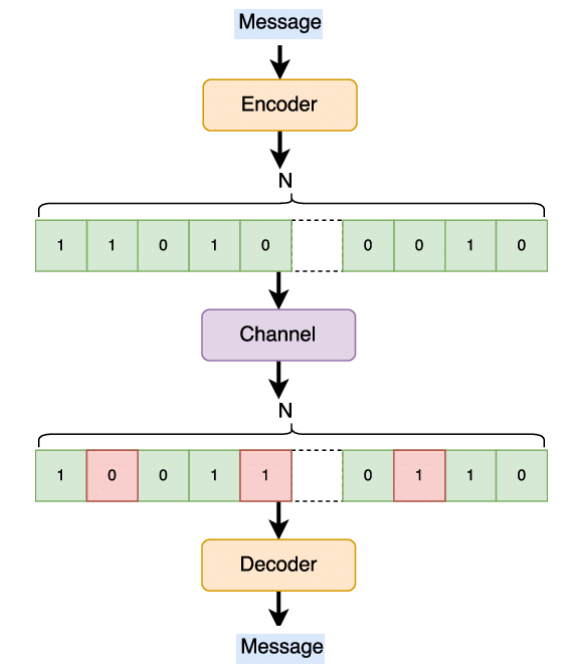
\includegraphics[width=0.5\textwidth]{images/section_1/code_base.png}
  \caption{Code-based cryptography}
  \label{fig:code-based}
\end{figure}

\noindent
Code-based cryptography is a type of post-quantum cryptography that relies on the \underline{hardness of decoding random linear codes} \\
The most well-known code-based cryptosystem is the McEliece cryptosystem, which was proposed in 1978. It is based on the difficulty of decoding a general linear code, which is believed to be resistant to quantum attacks.


\subsubsection{Lattice based cryptography}

\begin{figure}[h!]
  \centering
  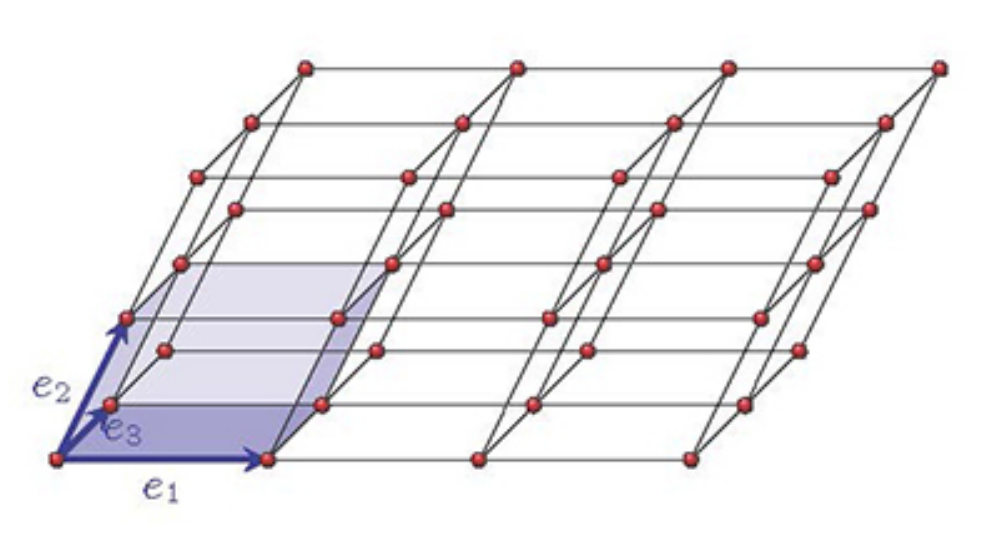
\includegraphics[width=0.75\textwidth]{images/section_1/lattice}
  \caption{Lattice based cryptography}
  \label{fig:lattice-based}
\end{figure}

Lattice based cryptography is another approach to post-quantum cryptography that relies on the hardness of certain problems in lattice theory, such as the shortest vector problem (SVP), the closest vector problem (CVP) and the learning with errors (LWE) problem. \\
These problems are believed to be resistant to quantum attacks and have gained significant attention in recent years.

\subsubsection{Multivariate cryptography}


\begin{align*}
f_1(x_1, \dots, x_n) &= \sum_{1 \leq i \leq j \leq n} a_{ij}^{(1)} x_i x_j + \sum_{1 \leq i \leq n} b_i^{(1)} x_i + c^{(1)} = 0, \\
\vspace{1cm}
f_2(x_1, \dots, x_n) &= \sum_{1 \leq i \leq j \leq n} a_{ij}^{(2)} x_i x_j + \sum_{1 \leq i \leq n} b_i^{(2)} x_i + c^{(2)} = 0, \\
\vspace{0.5cm}
&\vdots \\
\vspace{0.5cm}
f_m(x_1, \dots, x_n) &= \sum_{1 \leq i \leq j \leq n} a_{ij}^{(m)} x_i x_j + \sum_{1 \leq i \leq n} b_i^{(m)} x_i + c^{(m)} = 0.
\end{align*} 

\noindent
Multivariate cryptography is a third approach to post-quantum cryptography that relies on the hardness of solving systems of multivariate polynomial equations of degree at least two. 


\subsection{NIST standardization}
In 2017, NIST (National Institute of Standards and TechnologyUSA) opened a call for submitting new post-quntum cryptographic schemes and digital signatures, with three rounds, divided into:
\begin{itemize}
\item Key Encapsulation Mechanism (KEM)
\item Digital Signatures
\end{itemize}

\noindent
Initially, 82 proposals were submitted to the NIST PQC competition, and 69 were admitted to the first round. In July 2022, NIST announced the selected algorithms after the third round.

\paragraph{Selected Algorithms (Round 3)}

\begin{itemize}
    \item \textbf{Lattice-based}
    \begin{itemize}
        \item \textbf{KEM}: CRYSTALS-Kyber
        \item \textbf{Digital Signatures}: CRYSTALS-Dilithium, Falcon
    \end{itemize}
    
    \item \textbf{Hash-based}
    \begin{itemize}
        \item \textbf{Digital Signatures}: SPHINCS+
    \end{itemize}
\end{itemize}

\paragraph{Round 4 Candidates}

\begin{itemize}
    \item \textbf{Code-based KEM}: BIKE, Classic McEliece, HQC
    \item \textbf{Isogeny-based}: SIKE (broken in August 2022)
\end{itemize}

\paragraph{New NIST Call for Digital Signatures (2024)}

\noindent
After the first round (October 2024), 14 signature schemes remain in the competition:

\begin{itemize}
    \item \textbf{Lattice-based}: HAWK
    \item \textbf{Code-based}: CROSS, LESS
    \item \textbf{MPC-in-the-Head}: Mirath, MQOM, PERK, RYDE, SDitH
    \item \textbf{Multivariate}: MAYO, QR-UOV, SNOVA, UOV
    \item \textbf{Isogeny-based}: SQIsign
    \item \textbf{Symmetric-based}: FAEST
\end{itemize}


\newpage

\subsection{NOT-Covered Hard Problem}
The following hard problems are not covered in this course, but they are also important in the context of post-quantum cryptography:

\subsubsection{Hash based cryptography}

\begin{figure}[h!]
  \centering
  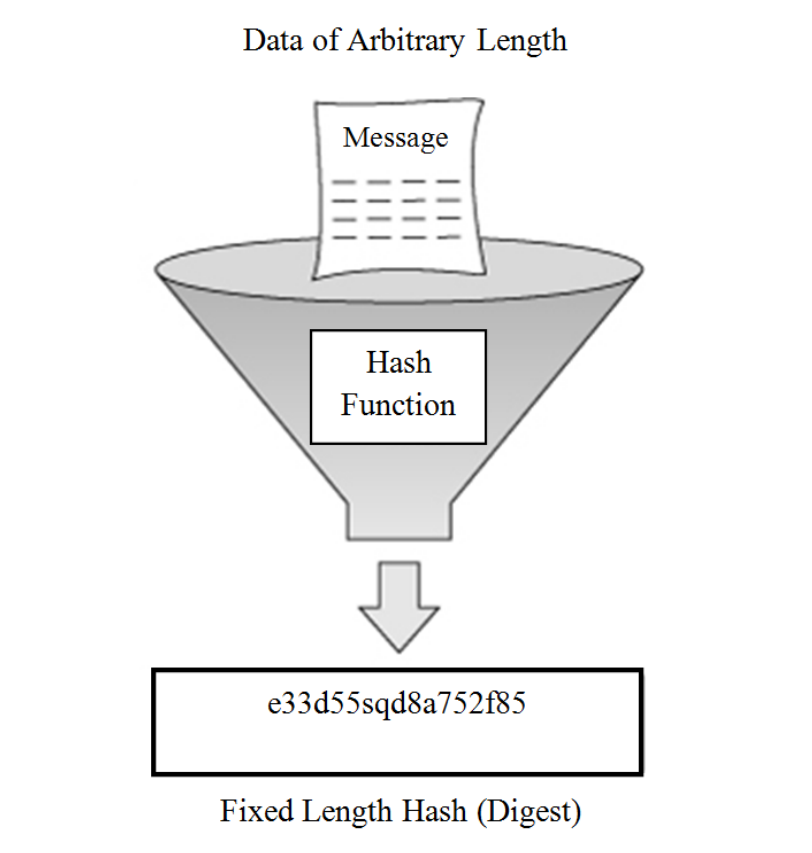
\includegraphics[width=0.5\textwidth]{images/section_1/hash_based.png}
  \caption{Hash based cryptography}
  \label{fig:hash-based}
\end{figure}

\noindent
Hash-based cryptography relies on the hardness of finding collisions in hash functions. It is a well-studied area of post-quantum cryptography, and several hash-based signature schemes have been proposed, such as the Merkle signature scheme and the SPHINCS.

\subsubsection*{Isogeny based cryptography}

\begin{figure}[h!]
  \centering
  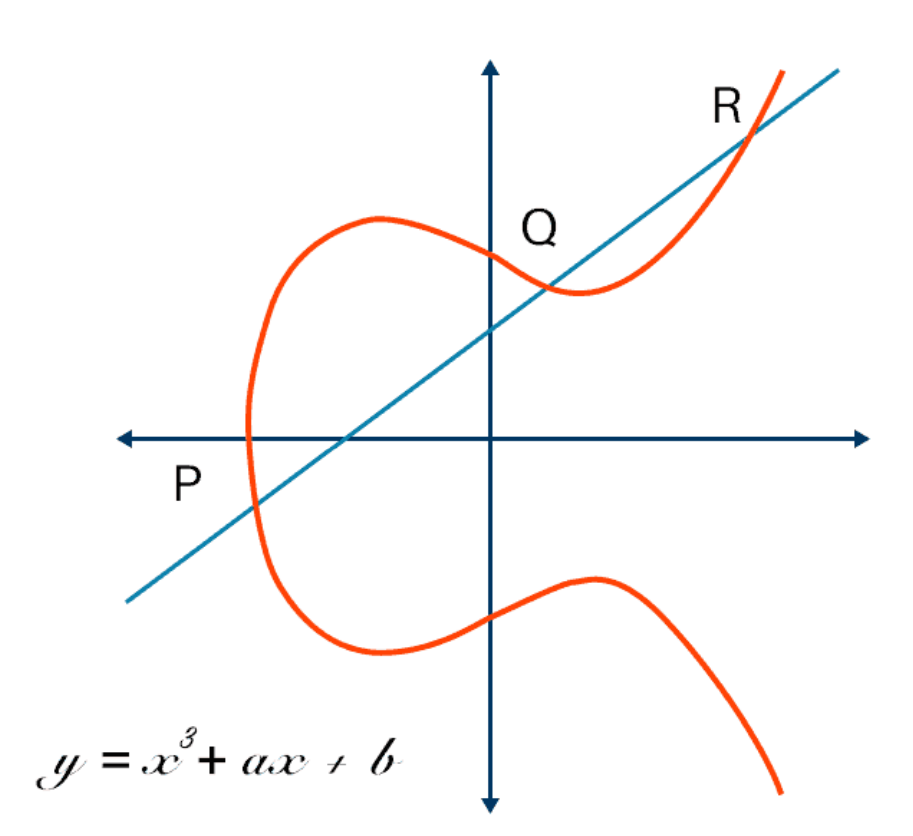
\includegraphics[width=0.5\textwidth]{images/section_1/isogeny.png}
  \caption{Isogeny based cryptography}
  \label{fig:isogeny-based}
\end{figure}

Isogeny-based cryptography relies on the hardness of finding isogenies between elliptic curves \textit{"given two elliptic curves, finding a path between them"}. It is a relatively new area of post-quantum cryptography, and several isogeny-based schemes have been proposed, such as the Supersingular Isogeny Key Exchange (SIKE) protocol [recently broken in August 2022].

\newpage

\subsection{Focus: Quantum Notation}
\[
|\psi\rangle = a|0\rangle + b|1\rangle,
\qquad a,b \in \mathbb{C}
\]

\[
|a|^2 + |b|^2 = 1
\]

\[
|0\rangle =
\begin{pmatrix}
1 \\
0
\end{pmatrix},
\qquad
|1\rangle =
\begin{pmatrix}
0 \\
1
\end{pmatrix}
\]

\[
|\psi\rangle =
a
\begin{pmatrix}
1 \\
0
\end{pmatrix}
+
b
\begin{pmatrix}
0 \\
1
\end{pmatrix}
=
\begin{pmatrix}
a \\
b
\end{pmatrix}
\in \mathbb{C}^2
\]

\[
|\psi\rangle =
\frac{1}{\sqrt{2}}|0\rangle +
\frac{1}{\sqrt{2}}|1\rangle
=
\frac{1}{\sqrt{2}}
\begin{pmatrix}
1 \\
1
\end{pmatrix}
\]

\noindent
In quantum computing, the state of a qubit is represented as a linear combination of the basis states $|0\rangle$ and $|1\rangle$, where the coefficients $a$ and $b$ are complex numbers that satisfy the normalization condition $|a|^2 + |b|^2 = 1$. The basis states can be represented as column vectors, and the state of the qubit can be expressed as a vector in a two-dimensional complex Hilbert space.




\def\slides{slides/sample-2.pdf}
\section{Recap of Algebra}

\subsection{Group}
\begin{defBox}{Group}
AAn algebraic structure $(G, *)$, where $G$ is a set and $*$ an operation between elements of $G$, i.e, a function $* : G \times G \to G$, is a group if it satisfies the following properties:
\begin{itemize}
    \item \textbf{* is associative}: $\forall g_1, g_2, g_3 \in G$, we have $(g_1 * g_2) * g_3 = g_1 * (g_2 * g_3)$.
    \item \textbf{Identity element}: There exists an element $e \in G$ such that $\forall a \in G$, we have $e * a = a * e = a$.
    \item \textbf{Inverse element}: $ \forall a \in G$, there exists an element $h \in G$ such that $a * h = h * a = e$.
\end{itemize}
\end{defBox}

\noindent
If $*$ is commutative, i.e., $\forall g_1, g_2 \in G$, we have $g_1 * g_2 = g_2 * g_1$, then the group is called \textit{abelian}.

\bigskip

\noindent
Typically, we use the following notations for groups:

\begin{table}[H]
\centering
\begin{tabular}{cc}
\toprule
\textbf{Additive Notation} & \textbf{Multiplicative Notation} \\
\midrule

$(G, +)$ & $(G, \cdot)$ \\[6pt]

$0$ is the identity & $1$ is the identity \\[6pt]

$-g$ is the inverse of $g$ & $g^{-1}$ is the inverse of $g$ \\[6pt]

$Ng = \underbrace{g + \dots + g}_{N\ \text{times}}$
&
$g^N = \underbrace{g \cdot \dots \cdot g}_{N\ \text{times}}$

\\
\bottomrule
\end{tabular}
\caption{Additive and multiplicative notation for group operations}
\end{table}

\begin{quote}
\textbf{Author's Note:} The Professor underlined that it is just a notation. For istance with the $0$ we don't mean the number $0$, but the identity element of the group, and with $-g$ we don't mean the negative of $g$, but the inverse of $g$.
\end{quote}


\begin{defBox}{Cyclic Group}
AA group $G$ is called \textit{cyclic} if there exists (at least) an element $g \in G$ such that:\\
$G = <g> = (g)$ where $<g> = (g) = \{g^k : k \in \mathbb{Z}\} = \{kg : k \in \mathbb{Z}\}$ \\
i.e., $G$ is generated by $g$ and $g$ is called a \textit{generator} of $G$.
\end{defBox}

\medskip

\begin{defBox}{Subgroup}
AA subgroup $H$ of a group $G$ is a subset of $G$ that is itself a group under the operation of $G$.
\end{defBox}

\subsubsection*{Examples}
\begin{itemize}
    \item $(\mathbb{N}, +)$ is NOT a group because it lacks inverses.
    \item $(\mathbb{Z}, +)$ is a cyclic group generated by $1$ (or $-1$).
    \item $(\mathbb{Q}, \cdot)$ is NOT a group because number $0$ does not have a multiplicative inverse.
\end{itemize}
In general, we use x or $*$ for "restructing" a set to invertible elemts
\begin{itemize}
    \item $(\mathbb{Q}^x, \cdot)$ is a group, where $\mathbb{Q}^x = \mathbb{Q} \setminus \{0\}$
    \item $(\mathbb{Z}^x, \cdot)$ is a group, where $\mathbb{Z}^x = \{ \pm 1\}$    
\end{itemize}

\bigskip

\noindent
In cryptography it is essential know $$\mathbb{Z}_n = \{0, 1, \dots, n-1\}$$ that is the set of all remainders, the division by a fixed integer $N (N>1)$.\\
$\mathbb{Z}_n$ is constructed starting from $\mathbb{Z}$, and introducing a relation of equalence among integers:\\
- given $a, b \in \mathbb{Z}$, we say that $a$ and $b$ are equivalent modulo $N$ if $N$ divides $a-b$, i.e., if there exists an integer $k$ such that $a - b = kN$.\\
In this way we can partition $\mathbb{Z}$ into $N$ equivalence classes, and each class can be represented by one of its elements, called a \textit{representative}.

\bigskip

\noindent


\begin{defBox}{Invertible Element}
AAn element $a \in \mathbb{Z}_n$ is \textbf{invertible} with respect to multiplication if and only if $gcd(a, n) = 1$.
\end{defBox}

\noindent
Indeed, if $gcd(a, n) = 1$, then by the \textit{Bezout's identity} there exist two integers $x$ and $y$ such that $ax + ny = 1$, and thus $ax \equiv 1 \mod n$, beacause $ny \equiv 0 \mod n$.\\
Consequently $x$ is the inverse of $a$ with respect to product.\\
On the other hand, if $gcd(a, n) = d \neq 1$, then $a$ is \underline{not} invertible with respect to the product.\\
Indeed, in this case we have $a= d \cdot a'$, $N = d \cdot N'$ and f we suppone by absurd that $a$ is invertible we get a contraddiction: 
\begin{align*}
    ax &\equiv 1 \mod n \implies \\
    d \cdot a' x &\equiv 1 \mod d \cdot N \implies \\
    N'da'x &\equiv N' \mod N  \implies \\
    Na'x &\equiv N' \mod N \implies \\
    0 &\equiv N' mod N
\end{align*}
\indent
but $N' \neq 0$ and $N' < N$, thus we have a contraddiction.\\

\begin{defBox}{Euler's Totient Function}
    TThus $\mathbb{Z}^x_n = \{ a\in \mathbb{Z}_n : gcd(a,n) = 1 \}$  and we define $\varphi(n) = |\mathbb{Z}^x_n|$ as the number of invertible elements in $\mathbb{Z}_n$.
    \medskip

    \noindent
    The Euler totient function satisfies the following properties:
    \begin{itemize}
        \item If $p$ is a prime number, then $\varphi(p) = p-1$.
        \item If $p$ is a prime number and $k$ is a positive integer, then $\varphi(p^r) = p^r - p^{r-1} = p^r (1 - \frac{1}{p})$.
        \item If $a$ and $b$ are coprime positive integers, then $\varphi(ab) = \varphi(a) \cdot \varphi(b)$.
    \end{itemize}
\end{defBox}

\noindent
\textbf{IMPORTANT:} If we know the factorization of $N$, we can compute $\varphi(N)$, and viceversa.\\
\noindent 
So, compute $\varphi(N)$ is as hard as factor $N$.\\
This is the reason why $\varphi(N)$ is used in RSA, and why the security of RSA relies on the hardness of factorization.\\
\bigskip

\noindent
Given $a \in \mathbb{Z}^x_n$, i.e., $gcd(a,n) = 1$, we can find its inverse usign the Bezout's identity which can be determined by means of the \textbf{Extended Euclidean Algorithm}.\\
The time complexity of the Extended Euclidean Algorithm is $O(\log n)$, thus we can compute the inverse of an element in $\mathbb{Z}^x_n$ in polynomial time.
\medskip

\noindent
Indeed, the Euclidean algo. starts computing $N= qa+r$ where $0 \leq r < N$ and we can continue until we get a remainder euqal to 0.\\
Thus, first of all, it is immediate to see that the time complexity is $O(a)$ or $O(N)$ since $a<N$. BUT WE CAN DO BETTER!
\medskip

\noindent
In fact, in a general step of the Euclidean algo. we get somthing like\\
$r_{i-2} = q_i r_{i-1} + r_i \geq r_i + r_{i+1}$ 
\smallskip

\noindent
Now, assume that we performed $t$ steps, then we have $r_{t+1}=0$ and $r_t \neq 0$:
\begin{align*}
    r_t \geq 1 &= F_1 \\
    r_{t-1} \geq r_t + r_{t+1} &= r_t \geq 1= F_2\\
    r_{t-2} \geq r_{t-1} + r_t &\geq F_2+F_1=F_3\\
    &\vdots \\
    a > r_1 \geq F_t \geq \phi^{t-2}
\end{align*}
where $\phi = \frac{1+\sqrt{5}}{2}$ is the \textbf{golden ratio}\\
and, where $F_1, F_2, F_3, \dots$ are the \textbf{Fibonacci numbers}.\\
Thus, $\phi^{t-2} \leq a \implies \log_\phi \phi^(t-2) < \log_\phi a \implies t-2 < \log_\phi a \implies t \sim O(\log a) \sim O(\log N)$.

\vspace{0.5 cm}

\noindent\rule{\textwidth}{0.5pt}

\vspace{0.5 cm}

\noindent
So, by previous explanations, we can determinate that: $(\mathbb{Z}_N, +)$ is a cycling group, indeed $1$ is a generator: $<1> = \mathbb{Z}_N$
\smallskip

\noindent
All the generators of $\mathbb{Z}_N$ are teh elements $a \in \mathbb{Z}_N$ such that $gcd(a,N) = 1$:\\
$<a> = \{ ka \in  \mathbb{Z}_N : k \in \mathbb{Z} \} = \mathbb{Z}_N$ where $ka = \frac{a+...+a}{k}$

\medskip

\noindent
\textbf{Example}\\
Consider $ (\mathbb{Z}_{12}, +)$:

\begin{itemize}
    \item $<1> = \{ 1, 2, 3, 4, 5, 6, 7, 8, 9, 10, 11\} = \mathbb{Z}_{12}$
    \item $<2> = \{ 2, 4, 6, 8, 10, 0\} \	\subseteq \mathbb{Z}_{12}$
    \item $<3> = \{ 3, 6, 9, 0\} \subseteq \mathbb{Z}_{12}$
    \item $<4> = \{ 4, 8, 0\} \subseteq \mathbb{Z}_{12}$
    \item $<5> = \{ 5, 10, 3, 8, 13, 6, 11, 4, 9, 2, 7, 0   \} \subseteq \mathbb{Z}_{12}$   
\end{itemize}
\noindent
By analyzing the last example (<5>), we can see that $5 \equiv 0 \mod 12$, so we can generalize that:\\
$5k \equiv 0 \mod 12 \iff k$ is multiple of 12.
\bigskip

\noindent
\textbf{Remark}\\
The number oof generators of $\mathbb{Z}_N$ is $\varphi(N)$.

\begin{defBox}{Morphism}
    GGiven a function $f: (G, *) \to (G', *')$, then $f$ is a morphism if $\forall g_1, g_2 \in G$, we have $f(g_1 * g_2) = f(g_1) *' f(g_2)$.
\end{defBox}

\noindent
A biejective morphism is called an \textbf{isomorphism}.

\begin{thmBox}{Isomorphism of Cyclic Groups}
    a\begin{itemize}
        \item A cycling group with infintely many elements is isomorphic to $(\mathbb{Z}, +)$.
        \item A cycling group with $N$ elements is isomorphic to $(\mathbb{Z}_N, +)$.
    \end{itemize}
\end{thmBox}

\noindent
The \underline{idea of proof:}\\ 
Consider a cyclic group $G$ with infintely many elements:\\
Let $g$ be a generator of $G$, then we can define a function $f: \mathbb{Z} \to G$ such that $f(k) = kg$.\\
It is easy to see that $f$ is a morphism, indeed $f(k_1 + k_2) = (k_1 + k_2)g = k_1g + k_2g = f(k_1) + f(k_2)$.\\
Moreover, $f$ is injective, indeed if $f(k_1) = f(k_2)$, then $k_1g = k_2g$, and since $g$ is a generator, we have $k_1 = k_2$.\\
Finally, $f$ is surjective, indeed for every $h \in G$, there exists $k \in \mathbb{Z}$ such that $h = kg$, thus $f(k) = h$.\\
\bigskip    

\noindent
\textbf{Remark:}\\
$(\mathbb{Z}^x_N , \cdot)$ is a cycling group $\iff$ $N = 2, 4, p^k, 2p^k$ where $p$ is an odd prime and $k \geq 1$.\\
Thus, in this case we have $(\mathbb{Z}^x_N , \cdot) \simeq (\mathbb{Z}_{\varphi(N)}, +)$.

\bigskip

\begin{defBox}{Kernel}
    GGiven a morphism $f: (G, *) \to (G', *')$, the kernel of $f$ is the set of elements of $G$ that are mapped to the identity element of $G'$, i.e., $\text{Ker}(f) = \{ g \in G : f(g) = e' \}$ where $e'$ is the identity element of $G'$.
\end{defBox}

\begin{quote}
    Author's Note: I use the letter $e$ (for semplicity) for the identity element of $G$. If we want to follow the Murru's notation, we should use $1_G$ 
\end{quote}

\begin{propBox}{Kernel injectivity}
    a$f$ is injective $\iff$ $\text{Ker}(f) = \{ e \}$ where $e$ is the identity element of $G$.
\end{propBox}
\medskip
\begin{defBox}{Subgroup Characterization}
    LLet $G$ be a group, then $H \subseteq G$ is a subgroup of $G$ if and only if $H$ is a group with respect to the operation of $G$.
\end{defBox}

\medskip

\begin{propBox}{Subgroup Test}
    a$H \subseteq G$ is a subgroup $\iff \forall h_1, h_2 \in H$, we have $h_1 * h_2^{-1} \in H$.
\end{propBox}

\medskip

\noindent
\textbf{Example:}\\
Consider $G = (\mathbb{Z}, +)$, then the subgroups of $G$ are the following set:\\
$<N> = (N) = N\mathbb{Z} = \{ kN: k \in \mathbb{Z} \} $ (the set of all multiples of $N$)\\
\smallskip

\noindent
Indeed, given $h_1, h_2 \in N\mathbb{Z}$, we have that $h_1 - h_2 = k_1N - k_2-N = (k_1 - k_2)N \in N \mathbb{Z}$.\\
Thus, $N\mathbb{Z}$ is a subgroup of $(\mathbb{Z}, +)$. On the other hand, any subset $H$ of $\mathbb{Z}$ is of the kind $N\mathbb{Z}$.\\
\smallskip
\noindent
Consider $H \subseteq \mathbb{Z}$ with $H \neq \{0\}$, thus $H$ must contain at least one positive integer $N$.\\
Let $N$ be the smallest positive integer in $H$ (no zero), then we have that $N\mathbb{Z} \subseteq H$, because $H$ must be closed under +.
\smallskip

\noindent
Now, consider $m \in H$ and let us divide it by $N$: $m = qN + r$ with $0 \leq r < N$.\\
$\implies r= m - qN \in H \implies r= 0$ (becauuse N is the smallest positive integer in $H$).\\
$\implies m $ is a multiple of $N$, thus $H \subseteq N\mathbb{Z}$.

\bigskip

\begin{thmBox}{Lagrange's Theorem}
    aGiven a finite group $(G, *)$ and a subgroup $H \leq G$, then $|H| \mid |G|$.\\
    Where $|H|$ and $|G|$ are the number of elements of $H$ and $G$ respectively.
\end{thmBox}

\noindent
\textbf{Corollary:}\\
If $|G| = n$, then $\forall g \in G$, we have $g^n = 1$ or $ng = 0$ depending on the notation we use for the group operation.\\

\begin{thmBox}{Euler's Theorem}
    a$a \in \mathbb{Z}^x_N$, then $a^{\varphi(N)} \equiv 1 \mod N$.
\end{thmBox}

\medskip

\begin{thmBox}{Fermat's Little Theorem}
    a$a \in \mathbb{Z}^x_p$, p prime, then $a^{p-1} \equiv 1 \mod p$.
\end{thmBox}

\newpage

\subsection{Rings}

\begin{defBox}{Rings}
    GGiven an algebraic structure $(R, *_1, *_2)$,then $R$ is a ring if:

    \begin{itemize}
        \item $(R, *_1)$ is an abelian group.
        \item $*_2$ is associative, $*_2$ is commutative (only for our purposes), and $*_2$ has an identity element with respect to $*_2$.
        \item Distrubutive property: $\forall a, b, c \in R$, we have $a *_2 (b *_1 c) = (a *_2 b) *_1 (a *_2 c)$ and $(b *_1 c) *_2 a = (b *_2 a) *_1 (c *_2 a)$.
    \end{itemize}
\end{defBox}

\noindent
Usually we use the following notations for rings: $(R, +, \cdot)$\\
\\
\textbf{Examples:}
\begin{itemize}
    \item $(\mathbb{Z}, +, \cdot)$ is a ring of integers.
    \item $(\mathbb{Z}_N, +, \cdot)$ is a ring of resuders modulo $N$.
\end{itemize}
\medskip

\noindent
For the groups, we have constructed $\mathbb{Z}_N$ starting from $\mathbb{Z}$, and introducing a relation of equivalence among integers.\\
In particular, we verified that $a \sim b \iff a \equiv b \mod N$.
\medskip

\noindent
We can provide the same construction considering the ring $(\mathbb{Z}, +, \cdot)$ and the same relation of equivalence, that will determinate the new ring ($\mathbb{Z}_N, +, \cdot$) (we can aslo write $\mathbb{Z}_N \simeq \mathbb{Z} / N$)
\medskip

\noindent
When we introduce a relation of equivalence, we are also providing a partition of the set $\mathbb{Z}$ into equivalence classes, and each class can be represented by one of its elements, called a \textit{representative}.\\
$[0]$ is the class of all integers with remainder $0:...-2N, -N, 0, N, 2N, ...$\\
$[1]$ is the .... integers with remainder $1:...-2N+1, -N+1, 1, N+1, 2N+1, ...$\\
$[0] \cap [1] = \emptyset$ and $[0] \cup [1] \cup ... \cup [N-1] = \mathbb{Z}$\\
\bigskip

\noindent
We can obtain $\mathbb{Z}_N$ starting from $\mathbb{Z}$ in a differten (equivalent) way.\\
Consider the ring $\mathbb{Z}, +, \cdot$, the following set $<N> = (N) = N\mathbb{Z} = \{ kN: k \in \mathbb{Z} \} $ (the set of all multiples of $N$) are a special subset of $\mathbb{Z}$, that satisfy the following properties:

\begin{itemize}
    \item $(N)$ is a subgroup of $(\mathbb{Z}, +)$
    \item $\forall a \in \mathbb{Z}$, $\forall b \in (N)$, we have $ab \in (N)$ where $(N)$ is the ideal of $(\mathbb{Z}, +, \cdot)$
\end{itemize}  
\smallskip

\noindent
If we fix an ideal $(N)$, then we can derive a relation of equivalence:\\
$a, b \in \mathbb{Z}$ are equivalent $a \sim b \iff a + (-b) \in (N)$ (this condition is the same as $a \equiv b \mod N$).
\medskip

\noindent
Then, $\mathbb{Z}_N$ is the set od class of equivalence with respect to this relation, and we can write $\mathbb{Z}_N = \mathbb{Z} / (N) = \mathbb{Z}_N / N\mathbb{Z}_N$

\newpage

\subsection{Field}
\begin{defBox}{Field}
    GGiven an algebraic structure $(F, +, \cdot)$, then $F$ is a field if:
    \begin{itemize}
        \item $(F, +)$ is an abelian group.
        \item $(F \setminus \{0\}, \cdot)$ is an abelian group where $0$ is the identity element of $(F, +)$.
        \item Distrubutive property: $\forall a, b, c \in F$, we have $a \cdot (b + c) = a \cdot b + a \cdot c$ and $(b + c) \cdot a = b \cdot a + c \cdot a$.
    \end{itemize}
\end{defBox}

\noindent
When a field has a finitely many elements, we call it a \textbf{finite field} or \textit{Galois field}.\\
\medskip

\noindent
\textbf{Examples:}\\
$(\mathbb{Z}_p[X], +, \cdot)$ is a ring, then $(f(X))= \{ g(x)f(x): g(x) \in \mathbb{Z}_p[X] \}$\\
$f(x)$ is invertible then $\mathbb{Z}_p[X] / (f(X))$ is a field

\bigskip

\begin{defBox}{Ideal}
    LLet $(R, +, \cdot)$ be a ring, then a subset $I \subseteq R$ is an ideal if:
    \begin{itemize} 
        \item $(I, +)$ is a subgroup of $(R, +)$
        \item $\forall r \in R$, $\forall i \in I$, we have $ri \in I$ and $ir \in I$.
    \end{itemize}
\end{defBox}

\noindent
Given an ideal, it is possible to define the following relation of equivalence: $a, b \in R$ are equivalent $a \sim b \iff a + (-b) \in I$, and we denote by $R/I$\\
This set is stilla a ring.
\medskip

\noindent
\textbf{Example:}\\
Consider the ring $(\mathbb{Z}, +, \cdot)$. The sets $(n)= n\mathbb{Z} = \{ kn: k \in \mathbb{Z} \}$ are ideals of $\mathbb{Z}$.
\smallskip

\noindent
Thus $\mathbb{Z}/(n) = \mathbb{Z}/n\mathbb{Z} = \mathbb{Z}$ is a new ring.\\
In this case, the relation of equivalence is:\\
$\forall a, b \in \mathbb{Z}, a \sim b \iff a + (-b) \in (n) \iff a - b = kn $ for some $k \in \mathbb{Z} \iff a \equiv b \mod n$
\bigskip\\
\noindent\rule{\textwidth}{0.5pt}


\noindent
If p is a prime number, the (p) is a special ideal called \textbf{maximal ideal}, (maximal ideal is an ideal that is not contained in any other ideal) and $\mathbb{Z}/ (p) = \mathbb{Z}/ p\mathbb{Z}$ is a field.
\medskip

\noindent
\textbf{Example:}\\
For example (5) is a maximal ideal, while (10) is not a maximal ideal, because (5) is an ideal that contains (10):
\begin{center}
    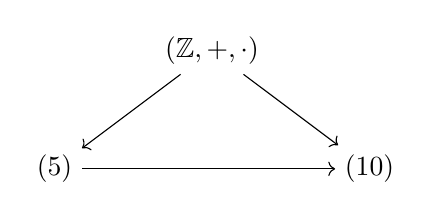
\begin{tikzpicture}
        \node (Z) at (0,0) {$(\mathbb{Z}, +, \cdot)$};
        \node (5) at (-2,-1.5) {$(5)$};
        \node (10) at (2,-1.5) {$(10)$};
        \draw[->] (Z) -- (5);
        \draw[->] (Z) -- (10);
        \draw[->] (5) -- (10);
    \end{tikzpicture}
\end{center}
\noindent
Because
\begin{align*}
    (5) &= \{ 5k : k \in \mathbb{Z} \} = \{ ..., -10, -5, 0, 5, 10, ...\} \\
    (10) &= \{ 10k : k \in \mathbb{Z} \} = \{ ..., -20, -10, 0, 10, 20, ...\}
\end{align*}
\noindent
and $(10) \subseteq (5)$ but $(5)$ is not contained in any other ideal.

\bigskip
\begin{thmBox}{Galois's Theorem on Finite Fields}
    LLet $\mathbb{F}_q$ be a finite field with $q$ elements, then we can only have the following situations:
    \begin{itemize}
        \item $q = p$ where $p$ is a prime number, and in this case $\mathbb{F}_q \simeq \mathbb{Z}_p$, so they are isomorphic.
        \item $q = p^k$ where $p$ is a prime number and $k$ is a positive integer, and in this case $\mathbb{F}_q \simeq \mathbb{F}_p[X] / (f(X))$ where $f(X)$ is an irreducible polynomial of degree $k$ over $\mathbb{F}_p$.
    \end{itemize}
\end{thmBox}

\bigskip

\noindent
\begin{defBox}{Irreducible Polynomial}
    aGiven a field $\mathbb{F}$, a polynomial $f(X) \in \mathbb{F}[X]$ is irreducible if it cannot be factorized into the product of two polynomials of degree >0 and <deg(f(x)).
\end{defBox}

\noindent
\textbf{Remark:}\\
Irreducible polynomials play the same role for polynomials as prime numbers play for integers.
\smallskip

\noindent
Given the ring $(\mathbb{Z}_p[x], +, \cdot)$ all and only the ideal are the sets\\
$(f(x)) = \{ g(x)f(x) : g(x) \in \mathbb{Z}_p[x] \} =$ {multiples of $f(x)$}\\
so, they are the analogue of the ideals $(n)$ for  $\mathbb{Z}$
\medskip

\noindent
If $f(x)$ is irreducible, then $(f(x))$ is a maximal ideal and $\mathbb{Z}_p[X] / (f(x))$ is a finite field with $p^k$ elements, where $k$ is the degree of $f(x)$.
\medskip

\noindent
Indeed, this is the set of classes of equivalence defined by\\
$\forall g_1(x), g_2(x) \in \mathbb{Z}_p[X], g_1(x) \sim g_2(x) \iff g_1(x) + (g_2(x)) \in (f(x)) \iff g_1(x) - g_2(x)  = g(x)f(x)$ for some $g(x) \in \mathbb{Z}_p[X] \iff g_1(x)$ and $g_2(x)$ have the same remainder with respect to the division by $f(x) \iff g_1(x) \equiv g_2(x) \mod f(x)$
\bigskip

\noindent
Thus $\mathbb{Z}_p[X] / (f(x))$ is the set of all possible reminders with respect to the division by $f(x)$, which are polynomials of degree < deg($f(x)$).\\
Indeed, given $h(x) \in \mathbb{Z}_p[X]$, we can write $h(x) = q(x)f(x) + r(x)$ where $r(x)$ is the remainder and $\deg(r(x)) < \deg(f(x))$.\\
\smallskip

\noindent
Thus a reminder, i.e., an element of $\mathbb{Z}_p[X] / (f(x))$, is a polynomial of kind $a_0 + a_1x + \cdots + a_{k-1}x^{k-1}$ where $a_i \in \mathbb{Z}_p$.\\
\smallskip
\noindent
Thus we have $p^k$ possible reminders, this is, $p^k$ possible elements in $\mathbb{Z}_p[X] / (f(x))$.\\


\newpage
\noindent
\textbf{Remark:}\\
Let $\mathbb{F}$ be a field:
\begin{itemize}
    \item if $f(x) \in \mathbb{F}[X]$ has a \underline{root} $\alpha \in \mathbb{F}$ (i.e., $f(\alpha) = 0$), then $f(x)$ is \underline{not} irreducible (it is irreducible). (*)
    \item if $f(x) \in \mathbb{F}[X]$ has degree 2 or 3 and has \underline{no root} in $\mathbb{F}$, then $f(x)$ is irreducible (if $\deg(f(x)) > 3$ and $f$ has no roots, we can not say anything)
\end{itemize}
\noindent
(*) Remember that if $\alpha$ is a root of $f(x)$, then $f(x) = (x - \alpha)g(x)$

\medskip
\begin{propBox}{Irreducibility}
    aA polynomia $f(x) \in \mathbb{Z}_p[X]$ of degree $k$ is irreducible if and only if:
    \begin{itemize}
        \item $f(x) | x^{p^k} - x$
        \item $\forall$ prime $r | k, gcd(f(x), x^{p^{k/r}} - x) = 1$ 
    \end{itemize}
\end{propBox}
\noindent
This proposition works well if $k$ is small (and it can be used very often in the construction of finite fields).\\
In general, it is not efficient  because we need to know the factorization of $k$. But there exist some efficient test for checking the irreducibility of a polynomial.

\noindent\rule{\textwidth}{0.5pt}

\noindent
\paragraph{BIG EXAMPLE: Construction of $\mathbb{F}_4$} 
\noindent
$\mathbb{F}_4 = \mathbb{F}_2$, thus we need to construct $\mathbb{F}_2[X] / (f(X))$ where $f(X)$ is an irreducible polynomial of degree 2 over $\mathbb{F}_2$.
\smallskip

\noindent
Remember that we are working in $\mathbb{F}_2[X]$, thus a polynomial of degree 2 is of the kind $ax^2 + bx + c$ where $a, b, c \in \mathbb{F}_2$.
\smallskip
\noindent
Thus, $a$ can be only equal to $1$ (otherwise the polynomial does not have degree 2)\\
$b, c \in \{0, 1\}$, thus we have 4 possible polynomials of degree 2:
\medskip

\noindent
$x^2, x^2 + 1, x + 1, x^2 + x + 1$
\begin{itemize}
    \item $x^2$ is not irreducible because it has a root (0)
    \item $x^2 + 1 = (x + 1)(x + 1) = (x + 1) ^2$ is not irreducible (1 is a root)
    \item $x^2 + x = x(x + 1)$ is not irreduucible (0 and 1 are roots)
    \item $x^2 + x + 1$ is irreducible (it has no roots in $\mathbb{F}_2$)
\end{itemize}

\medskip

\noindent
Thus $\mathbb{F}_4 = \mathbb{F}_2[X] / (x^2 + x + 1)$ = {reminders with respect to the division by $x^2 + x + 1$} = {all polynomials $\in \mathbb{F}_2[X]$ of degree < 2} = $\{ 0, 1,$ [poly of deg 0] $x, x+1 $[poly of deg 1] $\}$
\smallskip

\noindent
$\mathbb{F}_4 = \{ 0, 1, x, x+1 \} = \{ 0, 1, \alpha, \alpha+1 \}$ where $\alpha$ is a root in $\mathbb{F}_2$ of $x^2 + x + 1$ (somewhere else!)
\bigskip

\noindent
Let us observe that $x$ and $\alpha$ have the same behavior.\\
Indeed, $x^2 + x + 1$  is irreducible in $\mathbb{F}_4$, becasue $x^2 = 1(x^2+x+1) + x + 1$ where 1 is the quotient and $x + 1$ is the reminder.\\
Indeed, $x^2 + x + 1 + x + 1 = x^2 + 2x + 2 = x^2$ because we are working in $\mathbb{F}_2$ and $2x = 0$ and $2 = 0$.
\medskip

\noindent
On the other hand, it is possible to observe that:\\
$x^2 \equiv x^2 + x^2 + x + 1 \mod x^2+x+1 \implies x^2 \equiv 2x^2 + x + 1 \mod x^2 + x + 1 \implies x^2 \equiv x + 1 \mod x^2 + x+ 1$
\smallskip

\noindent
Similarly, since $\alpha$ is a root of $x^2 + x + 1$, we have $\alpha^2 + \alpha + 1 = 0 \implies \alpha^2 = - \alpha - 1 \implies \alpha^2 = \alpha + 1$.

\noindent
\textbf{End example}\\
other practial examples have been provided at lecture of 13-03-2026
\bigskip

\begin{defBox}{Primitive}
    aGiven $f(x) \in \mathbb{F}_p[X]$ if $f(x)$ is irreducible and \\
    $<x> = (\mathbb{F}_p[X]/(f(x)))^2$ then $f(x)$ is called primitive.
\end{defBox}
\bigskip

\begin{thmBox}{Cyclicality of Finite Fields}
    gGiven a finite field $\mathbb{F}_q$, then $(\mathbb{F}_q^x, \cdot)$ is a cyclic group.
\end{thmBox}

\noindent
These concepts are strictly related to the cryptographic applications, and they will be used in the construction of the AES (Advanced Encryption Standard) and in the construction of the elliptic curves.
\medskip

\noindent
For istance, \textbf{AES:}
\\
It is possible see AES consideing the fact that \textit{"bites are strings of bites of lenght 8. The number of possivle bytes is $2^8$"}\\
So $\mathbb{F}_2^8 = \mathbb{F}_2 \cdot \mathbb{F}_2 \cdots \mathbb{F}_2$ (8 times) VECTOR SPACE, but we can also see it as a field, because we can find an irreducible polynomial of degree 8 over $\mathbb{F}_2$, thus we can write\\
$\mathbb{F}_{2^8} = \mathbb{F}_2 [X] / (f(X))$ where $f(X)$ is an irreducible polynomial of degree 8 over $\mathbb{F}_2$.\\
$a_7x^7 + a_6x^6 + \cdots + a_1x + a_0$ where $a_i \in \mathbb{F}_2$ is the representation of a byte in AES (0, 1), and the operations of AES are defined as the operations of $\mathbb{F}_2[X] / (f(X))$.\\
\medskip

\noindent
In AES $\mathbb{F}_{2^8} \simeq \mathbb{F}_2[X] / (x^8 + x^4 + x^3 + x + 1)$ 


\begin{quote}
\textit{\textbf{Author's Note:} The Professor underlined that it is important, during individual study, to consider the difference between the two representations of $\mathbb{F}_{2^8}$, because they are equivalent but they have different properties.\\
In particular, the representation $\mathbb{F}_2^8$ is a vector space, thus it has a basis and we can represent the elements of $\mathbb{F}_{2^8}$ as linear combinations of the basis elements, while the representation $\mathbb{F}_2[X] / (f(X))$ is a field, thus it has a multiplicative structure and we can find the inverse of an element with respect to the multiplication.}
\end{quote}


\section{Linear Algebra}
Linear algebra is a branch of mathematics that studies vectors, vector spaces, and linear transformations, so linear objects.\\ It provides the foundation for many areas of mathematics and is essential in various applications, including cryptography.
\medskip

\noindent
For example, cosider $\mathbb{R}^2 = \mathbb{R}$ x $\mathbb{R} = \{(x,y) : x,y \in \mathbb{R}\}$\\
In $\mathbb{R}^2$, Euclidean plane, the most simple linear object are \underline{point} or equivalently \underline{vectors}.\\
\subsection{Vector}
Indeed, a point in $\mathbb{R}^2$  is indentified by pairs of real numbers. Indeed a vector is an "arrow" strating from the origin, thus a point, i.e., a pair of real numbers, indetifies also a vector.
\medskip

\begin{center}
    
    \begin{tikzpicture}

    % assi
    \draw[->] (-2,0) -- (3,0); % asse x
    \draw[->] (0,-2) -- (0,3); % asse y

    % origine
    \fill (0,0) circle (2pt);
    \node[below left] at (0,0) {$O$};

    % punto P
    \fill (2,2) circle (2pt);
    \node[above right] at (2,2) {$P$};

    % vettore OP
    \draw[->, thick] (0,0) -- (2,2);

    \end{tikzpicture}

\end{center}

\noindent
Formally:
\begin{defBox}{Vector}
    AA vector v$\in \mathbb{R}^n$ is a n-tuple of real numbers
        \begin{center}
            v = (v$_1$, v$_2$, ..., v$_n$)
        \end{center}
    
    \noindent
    With following operations:

        \begin{itemize}
        \item \textbf{Multiplication by a scalar}: tv = (tv$_1$, tv$_2$, ..., tv$_n$) for t $\in \mathbb{R}$ and v $\in \mathbb{R}^n$
        \item \textbf{Sum}: v + w = (v$_1$ +w$_1$, v$_2$ + w$_2$, ..., v$_n$ + w$_n$) for v,w $\in \mathbb{R}^n$
        \item \textbf{Dot product}: v $\cdot$ w = v$_1$w$_1$ + v$_2$w$_2$ + ... + v$_n$w$_n$ for v,w $\in \mathbb{R}^n$
        \item \textbf{Norm}: $\|v\| = \sqrt{v_1^2 + v_2^2 + \dots + v_n^2}$ for $v \in \mathbb{R}^n$
        \end{itemize}
\end{defBox}
\noindent
\textbf{Example:}\\
Let v = (2,-1,5) and w = ($\sqrt{2}$,$\frac{1}{3}$,0) be two vectors in $\mathbb{R}^3$.\\
Then:
\begin{itemize}
    \item $\frac{1}{2}$v = (1, -$\frac{1}{2}$, $\frac{5}{2}$)
    \item v + w = (2 + $\sqrt{2}$, -$\frac{2}{3}$, 5)
    \item $\|w\| = \sqrt{2 + \frac{1}{9} + 0} = \sqrt{\frac{19}{9}} = \frac{\sqrt{19}}{3}$
\end{itemize}

\begin{defBox}{Linear Independence}
   GGiven k vectors a$_1$, a$_2$, ..., a$_k$ in $\mathbb{R}^n$, they are \textbf{linearly dependent} if there exist scalars t$_1$, t$_2$, ..., t$_k$, not all zero, such that:
    \begin{center}
        t$_1$a$_1$ + t$_2$a$_2$ + ... + t$_k$a$_k$ = 0
    \end{center}
    Otherwise, they are \textbf{linearly independent}.\\
    This means that, if a$_1$, a$_2$, ..., a$_k$ are linearly independent, then we can write one of them as a linear combination of the others one
\end{defBox}
\noindent
This peculiarity is fundamental in cryptography, indeed, for example, in the case of the \textbf{LWE problem}, we have a system of linear equations, and the security of the scheme relies on the fact that these equations are linearly independent, thus we cannot solve them easily by simplify them one with the other much simpler.
\medskip

\noindent
\textbf{Example:}\\
Let us consider a$_1$ = (1, 0, -1, 1), a$_2$ = (2, 1, 0, -1), a$_3$ = (1, -1, -3, 4), a$_4$ = (2, 5, 0, -1).For instance, we have that a$_1$, a$_2$ and a$_3$ are linearly independent, while a$_4$ is linearly dependent on the others. \\
So:
\begin{center}
    3a$_1$ - a$_3$ - a$_4$ = 0
\end{center}
\noindent
and
\begin{center}
    a$_4$ = 3a$_1$ - a$_3$
\end{center}

\noindent
On the other hand, a$_1$, a$_2$ and a$_4$ are linearly independent, because:
\begin{center}
    xa$_1$ + ya$_2$ + za$_4$ = (x + 2y + 2z, y + 5z, -x, x - y - z) = (0, 0, 0, 0)
\end{center}
\noindent
if and only if x = y = z = 0, thus they are linearly independent.



\subsection{Lines}
A \textbf{line} in $\mathbb{R}^n$ can be defined as the set of points that can be expressed as a linear combination of a fixed point and a direction vector.\\
Considering a line in $\mathbb{R}^2$, it is a subset of $\mathbb{R}^2$ that can be expressed as:
\begin{center}
    y = mx + q with m, q $\in \mathbb{R}$
\end{center}
\medskip

\noindent
A linear can be also described in a parametric form as:
\begin{center}
    \[
    \begin{cases}
    x= tv_1 + x_A \\
    y= tv_2 + y_A
    \end{cases}
    \]
\end{center}
\noindent
This is the line through the point A = (x$_A$, y$_A$) and with direction the vector v = (v$_1$, v$_2$).

\subsubsection*{Linear objects in higher dimensions}
Similarly, in $\mathbb{R}^3$, we have the following linear object:
\begin{itemize}
    \item \textbf{Point/vectors}
    \item \textbf{Lines} --> described by two linear equations   \[
    \begin{cases}
    ax + by + cz + d =0 \\
    a^ix + b^iy + c^iz + d^i =0
    \end{cases}
    \]

    \item \textbf{Planes} --> described by one linear equation $ax + by + cz + d =0$
\end{itemize}

\noindent
These are only some of the linear objects, and we can also consider higher-dimensional linear objects.

\subsection{Matrix}
A \textbf{matrix} is a rectangular array of numbers, symbols, or expressions, arranged in rows and columns.\\
Formally:
\begin{defBox}{Matrix}
    GGiven m,n $\in \mathbb{N}$, a matrix A of size m x n is a table of $mn$ real numbers, arranged in m rows and n columns.
     \begin{center}
        \[
        A =
        \begin{pmatrix}
        a_{11} & a_{12} & \cdots & a_{1n} \\
        a_{21} & a_{22} & \cdots & a_{2n} \\
        \vdots & \vdots & \ddots & \vdots \\
        a_{m1} & a_{m2} & \cdots & a_{mn}
        \end{pmatrix}
        \]
    \end{center}
    \noindent
    Where a$_{ij} \in \mathbb{R}$ for all i = 1, 2, ..., m and j = 1, 2, ..., n.
\end{defBox}

\noindent
Sometimes, we write matrix using the following notation: $A = (a_{ij})$.
\bigskip

\noindent
\textbf{Classification:}\\
\begin{itemize}
    \item \textbf{Square matrix}: if m = n
    \item \textbf{Row vector}: if m = 1, so $\mathbb{R}^{1\times n}$
    \item \textbf{Column vector}: if n = 1, so $\mathbb{R}^{m \times 1}$
\end{itemize}
\bigskip

\noindent
\textbf{Operations on matrices:}\\
\begin{itemize}
    \item \textbf{Multiplication by a scalar:} tA = (ta$_{ij}$) for t $\in \mathbb{R}$ and A $\in \mathbb{R}^{m \times n}$
    \item \textbf{Sum:} A + B = (a$_{ij}$ + b$_{ij}$) for A, B $\in \mathbb{R}^{m \times n}$
    \item \textbf{Transpose:} A$^T$ = (a$_{ji}$) for A $\in \mathbb{R}^{m \times n}$, obteined by swapping rows and columns
    \item \textbf{Product:} AB = (c$_{ij}$) $\in \mathbb{R}^{m \times r}$, for all A $\in \mathbb{R}^{m \times n}$ and B $\in \mathbb{R}^{n \times r}$, where the elements c$_{ij}$ is obteined by performing the dot product between the i-th row of A and the j-th column of B
\end{itemize}

\noindent
\textbf{Example:}\\
Let A = $\begin{pmatrix}
    1 & 2 & 3 \\
    0 & 1 & -1
\end{pmatrix} \in \mathbb{R}^{2 \times 3}$ 
and B = $\begin{pmatrix}
    2 & 0 \\ 
    1 & 1 \\ 
    -1 & 3 \\ 
\end{pmatrix} \in \mathbb{R}^{3 \times 2}$
\medskip

\noindent
Then AB = $\begin{pmatrix} 
    1 & 11 \\
    2 & -2
\end{pmatrix} \in \mathbb{R}^{2 \times 2}$, 
BA = $\begin{pmatrix}
    2 & 4 & 6 \\
    1 & 3 & 2 \\
    -1 & 1 & -6 
\end{pmatrix} \in \mathbb{R}^{3 \times 3}$ 
\bigskip

\noindent
Given C = $\begin{pmatrix}
    5 & \sqrt{2} & \frac{1}{2} & 0\\
    -1 & 2 & \pi & -3
\end{pmatrix} \in \mathbb{R}^{2 \times 4}$, its trasponse is 
C$^T$ = $\begin{pmatrix}
    5 & -1 \\ 
    \sqrt{2} & 2 \\ 
    \frac{1}{2} & \phi \\ 
    0 & -3
\end{pmatrix} \in \mathbb{R}^{4 \times 2}$.

\begin{defBox}{Identity matrix}
    aThe identity matrix I$_n$ of size n x n is the square matrix with 1's on the main diagonal and 0's elsewhere.
     \begin{center}
        \[
        I_n =
        \begin{pmatrix}
        1 & 0 & \cdots & 0 \\
        0 & 1 & \cdots & 0 \\
        \vdots & \vdots & \ddots & \vdots \\
        0 & 0 & \cdots & 1
        \end{pmatrix}
        \]
    \end{center}
\end{defBox}

\subsubsection* {Important notions}
The \textbf{determinant} of a square matrix can be evaluted recursively.\\
Given a 2 x 2 matrix A = $\begin{pmatrix}
    a & b \\
    c & d
\end{pmatrix}$, its determinant is det(A) = ad - bc.\\
Given a 3 x 3 matrix B = $\begin{pmatrix}
    a & b & c \\
    d & e & f \\
    g & h & i
\end{pmatrix}$, \\ its determinant is det(B) = a det $\begin{pmatrix}
    e & f \\
    h & i
\end{pmatrix}$ - b det $\begin{pmatrix}
    d & f \\
    g & i
\end{pmatrix}$ + c det $\begin{pmatrix}
    d & e \\
    g & h
\end{pmatrix}$ = a(ei - fh) - b(di - fg) + c(dh - eg).\\
\bigskip 

\noindent
\textbf{Example:}\\
Given A = $\begin{pmatrix}
    2 & 0 & 1 & -3\\
    1 & 5 & -1 & 2\\
    4 & 1 & -2 & 7\\
    0 & 0 & 2 & 0
\end{pmatrix}$ then,
det(A) = -2 det $\begin{pmatrix}
    2 & 0 & -3 \\
    1 & 5 & 2 \\
    4 & 1 & 7
\end{pmatrix}$ and \\
det $\begin{pmatrix}
    2 & 0 & -3 \\
    1 & 5 & 2 \\
    4 & 1 & 7
\end{pmatrix}$ = 2 det $\begin{pmatrix}
    5 & 2 \\
    1 & 7
\end{pmatrix}$ - 3 det $\begin{pmatrix}
    1 & 5 \\
    4 & 1
\end{pmatrix}$ 
\bigskip

\noindent
The \textbf{trace} of a square matrix A = (a$_{ij}$) is the sum of the elements on the main diagonal, i.e., tr(A) = a$_{11}$ + a$_{22}$ + ... + a$_{nn}$.
\medskip

\noindent
\textbf{Example:}\\
Given 
\[
A = \begin{pmatrix}
2 & -1 & 0\\
4 & 3 & 5\\
1 & 2 & -2
\end{pmatrix}
\]
the trace is
\[
\operatorname{tr}(A) = 2 + 3 + (-2) = 3.
\]

\subsubsection{Matrix multiplication algorithms}
The standard algorithm for multiplying two n x n matrices has a time complexity of O(n$^3$).
\begin{algorithm}
\caption{Schoolbook Matrix Multiplication}
\begin{algorithmic}[1]

\Require Matrices $A \in \mathbb{R}^{n \times m}$, $B \in \mathbb{R}^{m \times p}$
\Ensure Matrix $C \in \mathbb{R}^{n \times p}$

\State Initialize $C$ as a zero matrix

\For{$i = 1$ to $n$}
    \For{$j = 1$ to $p$}
        \State $sum \gets 0$
        \For{$k = 1$ to $m$}
            \State $sum \gets sum + A_{ik} \cdot B_{kj}$
        \EndFor
        \State $C_{ij} \gets sum$
    \EndFor
\EndFor

\State \Return $C$

\end{algorithmic}
\end{algorithm}

\noindent
However, other algorithms exist:
\begin{itemize}
    \item \textbf{Strassen's algorithm} reduces the time complexity to O(n$^{2.807}$).\\
    \item \textbf{Coppersmith-Winograd algorithm} further reduces the time complexity to O(n$^{2.376}$).\\
    \item \textbf{Optimized CW-like algorithms} have been developed, achieving time complexities of O(n$^{2.373}$) 
\end{itemize}


\subsubsection{Matrix inversion algorithms}
A matrix is invertible if its determinant is non-zero.\\
The standard algorithm for inverting an n x n matrix (\textbf{Gauss-Jordan elimination})has a time complexity of O(n$^3$).

\begin{algorithm}
\caption{Gauss-Jordan}
\begin{algorithmic}[1]

\State Swapping two rows
\State Multiplying a row by a non-zero scalar
\State Adding a multiple of one row to another row

\end{algorithmic}

\end{algorithm}

\noindent
However, other algorithms exist:
\begin{itemize}
    \item \textbf{Strassen's algorithm} can be adapted for matrix inversion, achieving a time complexity of O(n$^{2.807}$).\\
    \item \textbf{Coppersmith-Winograd algorithm} can also be adapted for matrix inversion, achieving a time complexity of O(n$^{2.376}$).\\
    \item \textbf{Optimized CW-like algorithms} have been developed for matrix inversion, achieving time complexities of O(n$^{2.373}$).

\end{itemize}
\bigskip

\noindent
Professor Murru underlines that these algorithms are indeed polynomial-time. However, this can be misleading: in this context, the complexity is expressed in terms of the matrix dimension $n$, not in terms of the bit-length of the input. 
\medskip

\noindent
When considering the actual input size (i.e., the number of bits needed to represent the matrices), the complexity may become much larger in practice. Therefore, although these algorithms are polynomial in $n$, they are not necessarily efficient in the sense typically considered in cryptography, where efficiency is measured with respect to the bit-size of the input.

\subsubsection{Determinant algorithms}
The determinant of an n x n matrix can be computed using the standard algorithm (\textbf{Laplace expansion}) with a time complexity of O(n!).\\
However, more efficient algorithms exist:
\begin{itemize}
    \item \textbf{LU decomposition} can be used to compute the determinant in O(n$^3$) time.
    \item \textbf{Division-free algorithms} can compute the determinant in O(n$^3$) time without performing any division, which is particularly useful for integer matrices.
    \item \textbf{Fast matrix multiplication} can compute the determinant in O(n$^{2.373}$) time, leveraging fast matrix multiplication techniques.
    \item \textbf{Bareiss algorithm} is an efficient method for computing the determinant with a time complexity of O(n$^3$) and is particularly useful for integer matrices, as it avoids intermediate fractions.
\end{itemize}

\begin{algorithm}
\caption{Bareiss Algorithm}
\begin{algorithmic}[1]

\State \textbf{Input:} $M$ --- an $n \times n$ matrix, with non-zero leading principal minors
\State \textbf{Initialize:} $M_{0,0} \gets 1$

\For{$k = 1$ to $n-1$}
    \For{$i = k+1$ to $n$}
        \For{$j = k+1$ to $n$}
            \State $M_{i,j} \gets \dfrac{M_{i,j} M_{k,k} - M_{i,k} M_{k,j}}{M_{k-1,k-1}}$
        \EndFor
    \EndFor
\EndFor

\State \textbf{Output:} $M_{n,n}$ contains $\det(M)$

\end{algorithmic}
\end{algorithm}


%%less 19/03    

\subsection{Vector Space}

\begin{defBox}{vector space}
    aA \textbf{Vector space} over the real (or complex) numbers is a set V where there exists an operation between the elements of V that we denote by + and an operation between elements of V and elements of $\mathbb{R}$ (or $\mathbb{C}$) called multiplication by scalar, having good properties:

    \begin{itemize}
        \item + must be associative, there exists the identity, there exists the inverse, and it must be commutative
        \item Scalar multiplication must be associative and distributive with respect to the sum
    \end{itemize}
\end{defBox}
\medskip

\noindent
\textbf{Remark:}\\
The set $\mathbb{R}^n$ of vectors is a vector space over $\mathbb{R}$. The set $\mathbb{R}^{m \times n}$ of matrices is a vector space over $\mathbb{R}$, but we can also consider the set of matrices as a vector space over $\mathbb{C}$.
\bigskip

\noindent
Be careful: $\mathbb{R}^n$ is a vector space over $\mathbb{C}$, but it is not a vector space over $\mathbb{F}_q$, where $\mathbb{F}_q$ is a finite field with q elements, because the scalar multiplication is not defined for all scalars in $\mathbb{F}_q$.\medskip

\noindent
Consider, e.g., $\mathbb{R}^3$ and $\mathbb{F}_5$ and let see that $\mathbb{R}^3$ is not a vector space over $\mathbb{F}_5$.\\
Indeed, if we take the "scalar" 0$ \in \mathbb{F}_5$, and a non-zero vector v $ \in \mathbb{R}^3$ (i.e. v = (1, 2, 3)), then we have that 0$\cdot$ v = (0, 0, 0) and since 5=0 in $\mathbb{F}_5$, we have that 5$\cdot$ v = 0
\smallskip

\noindent
On the other hand, we can computer 5 $\cdot$ v also in the following way: 5$\cdot$ v = (1 + 1 + 1 + 1 + 1)v = v + v + v + v + v = (1, 2, 3) + ...+ (1, 2, 3) = (5, 10, 15) $\neq$ (0, 0, 0) $\in \mathbb{R}^3$.\\
because 5,10,15 are elements of $\mathbb{R}$, are not 0.
\bigskip

\noindent
Similarly, we can consider $\mathbb{F}_q^n$ as a vector space over $\mathbb{F}_q$, but we cannot consider $\mathbb{F}_q^n$ as a vector space over $\mathbb{R}$, because the scalar multiplication is not defined for all scalars in $\mathbb{R}$.\\
The main reason (without formal proof) is that:
\begin{itemize}
    \item $\mathbb{F}_q, q = p^k$ where p is primem has characteristic p, wich means that $\forall \alpha \in \mathbb{F}_q$, we have $\alpha + ....+ \alpha$ (p times) = 0
    \item $\mathbb{R}$ has characteristic 0, wich means that $\forall \alpha \in \mathbb{R} \setminus \{0\}, \alpha+...+ \alpha$ is always different from 0
\end{itemize}

\subsubsection{Basis}
In a vector space, there always exist a basis.

\begin{defBox}{Basis}
    aA basis is a set of vector that generate all the other ones by means of their linear combination.
\end{defBox}

\noindent
The vectors of a basis are linearly independent and they are set of generators of the vector space.\\
The number of vectors in a basis is called the \textbf{dimension} of the vector space.
\medskip

\noindent
\textbf{Example}\\
In $\mathbb{R}^3$, the standard basis is given by the vectors e$_1$ = (1, 0, 0), e$_2$ = (0, 1, 0) and e$_3$ = (0, 0, 1).

\subsubsection{Linear map}
A \textbf{linear map} (or linear transformation) is a function between two vector spaces that preserves the operations of vector addition and scalar multiplication.
\begin{center}
    \[
    f: V \rightarrow W
    \]
\end{center}

\noindent
where V and W are vector spaces , susch that for all u, v $\in V$ and t $\in \mathbb{R}$ (or $\mathbb{C}$), we have:
\begin{center}
    \[
    f(v_1 + v_2) = f(v_1) + f(v_2), f(kv) = kf(v)
    \]
\end{center}

\noindent
A linear map can be represented by a matrix f(v) = Av, where A is a matrix and v is a vector.
\medskip

\noindent
\textbf{Example:}\\
Consider f: $\mathbb{R}^2 \rightarrow \mathbb{R}^3$, such that
\begin{center}
    \[
    f(v) = w, w = (v_1 + v_2, v_3, 2v_4 - v_1, v_2 + 3v_3)
    \]
\end{center}
\noindent
This is a linear map, and it can be represented by the following matrix:
\begin{center}
    \[
    A = \begin{pmatrix}
    1 & 1 & 0 & 0 \\
    0 & 0 & 1 & 0 \\
    -1 & 0 & 0 & 1 \\
    0 & 1 & 3 & 0
    \end{pmatrix}
    \]
\end{center}

\subsubsection {Eigenvalues and eigenvectors}
Given a matrix A, or equivalently a linear map $f: V \rightarrow V$, a non-zero vector v is called an \textbf{eigenvector} of A if there exists a scalar $\lambda$ such that Av = $\lambda$v.\\
The scalar $\lambda$ is called the \textbf{eigenvalue} corresponding to the eigenvector v.
\medskip

\noindent
To compute the eigenvalues and eigenvectors of a matrix A, we can solve the characteristic equation det(A - $\lambda$I) = 0, where I is the identity matrix.\\
In this way, we can find the eigenvalues $\lambda$, and then we can find the corresponding eigenvectors by solving the equation (A - $\lambda$I)v = 0 for each eigenvalue $\lambda$.


\subsubsection{Tensor product}
The \textbf{tensor product} is a way to combine two vector spaces V and W into a new vector space V $\otimes$ W.

\begin{defBox}{Tensor product}
    aGiven two matrices A $\in \mathbb{R}^{m \times n}$ and B $\in \mathbb{R}^{p \times q}$, then their \textbf{Kronocker product} is:
    \begin{center}
        \[
        A \otimes B =
        \begin{pmatrix}
        a_{11}B & a_{12}B & \cdots & a_{1n}B \\
        a_{21}B & a_{22}B & \cdots & a_{2n}B \\
        \vdots & \vdots & \ddots & \vdots \\
        a_{m1}B & a_{m2}B & \cdots & a_{mn}B
        \end{pmatrix}
        \]
    \end{center}
    
\end{defBox}
\section{Coding Theory}
Coding theory is a branch of mathematics that studies the properties of codes, in particular it focuses on the \textbf{error-detection} and \textbf{error-correction} capabilities of codes. 


\begin{figure}[h!]
  \centering
  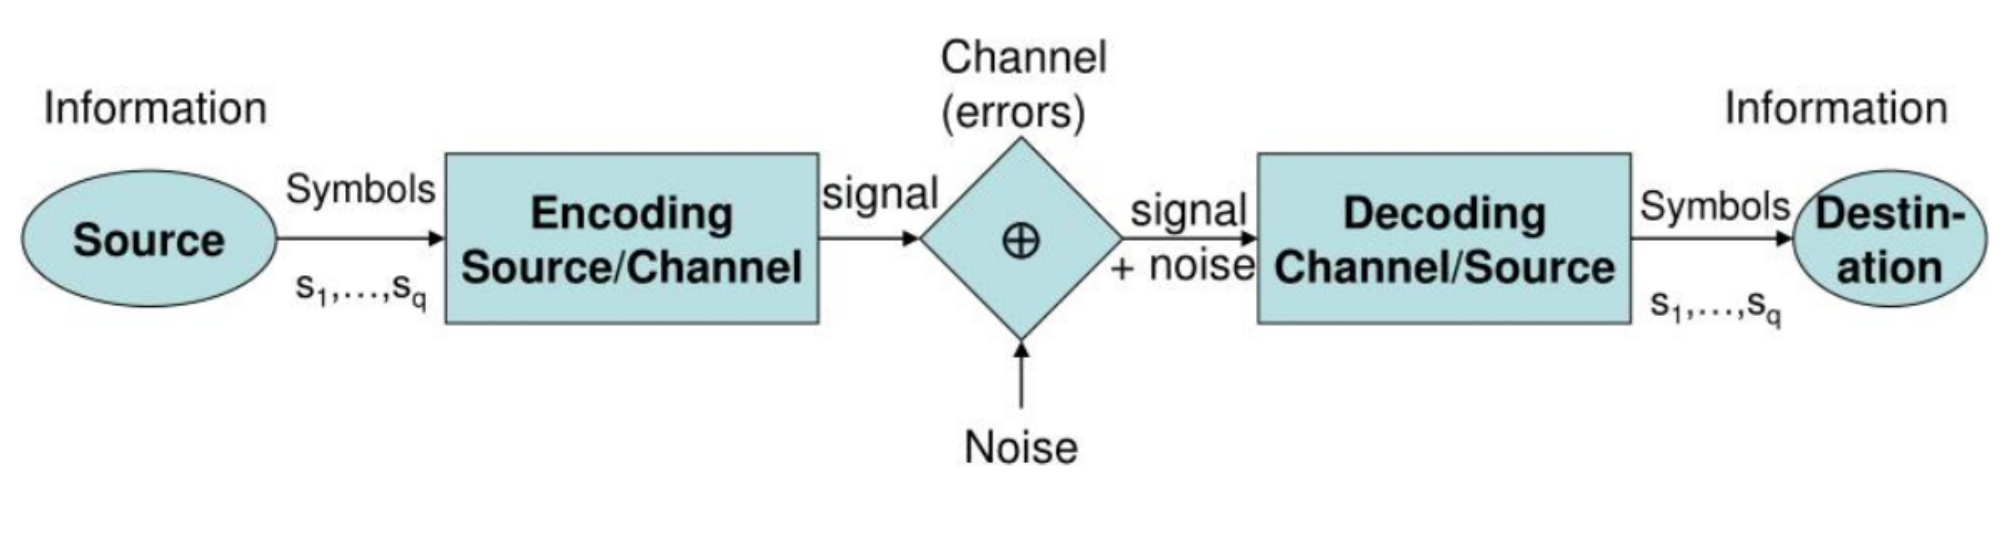
\includegraphics[width=1.2\textwidth]{images/section_4/coding_theory.png}
  \caption{Coding theory overview}
  \label{fig:coding-theory}
\end{figure}

\noindent
Each step shown in the figure above is crucial for the design and analysis of codes. The \textbf{encoding} step involves transforming the original message into a codeword using a specific encoding scheme. The \textbf{transmission} step is where the codeword is sent through a communication channel, which may introduce errors. The \textbf{decoding} step is where the received codeword is processed to recover the original message, and this is where error-detection and error-correction techniques come into play. \\
In the coding theory there are:

\begin{itemize}
    \item \textbf{$F$}: finite alphabet, which is the set of symbols used to construct codewords. For example, in binary codes, the alphabet is $\{0, 1\}$.
    \item \textbf{$m \in F^k$}: information word or message, which is the original data that we want to encode. It consists of $k$ symbols from the alphabet $F$.
    \item \textbf{$c \in F^n$}: codeword or input word, which is the encoded version of the message. It consists of $n$ symbols from the alphabet $F$, where $n \geq k$. 
    \item \textbf{$y \in F^n$}: received word or output word, which is the codeword that has been transmitted through the channel and may contain errors. It also consists of $n$ symbols from the alphabet $F$.
    \item \textbf{$\hat{c} \in F^n$} decoded word
    \item \textbf{$\hat{m} \in F^k$} decoded message
\end{itemize}

\subsection{Codewords}
For our purposes, we will consider \textbf{additive channels}, i.e., given c, y $\in F^n$, then
\begin{center}
    $y = c + e$
\end{center}
where $e$ is the error vector or error word. 
\medskip

\noindent
We define a (n, M)-code $C$ as  \underline{non empty subset of $F^n$ such that $|C| = n$} where $n$ is the \textbf{length} of the codewords and $M$ is the number of codewords in the code (\textbf{size}). \textit{(In this case the notation |C| doesn't mean "number of elemnts of C", but it means the leght of th vector)} \\
The quantity $k \coloneqq \log_{|F|} M$ is called the \textbf{dimension} or information length of the code and $R \coloneqq \frac{k}{n}$ is called the \textbf{rate} of the code.\\
The elements of $C$ are called \textbf{codewords}.

\subsubsection{Distances}

\begin{defBox}{Hamming Distance}
    GGiven x, y $\in F^n$, the Hamming distance between x and y is defined as the number of positions (coordinates) in which x and y differ.\\
    It is denoted as $d(x, y)$ 
\end{defBox}
\medskip

\begin{defBox}{Hamming Weight}
    AGiven x $\in F^n$, the Hamming weight of x is defined as the number of non-zero coordinates of x.\\
    It is denoted as $w(x)$
\end{defBox}
\medskip

\begin{defBox}{Minimum Distance}
    AGiven a (n, M)-code $C$, the minimum distance of $C$ is:
\begin{center}
    $d \coloneqq min\{d(c_1, c_2), \forall c_1, c_2 \in C, c_1 \neq c_2\}$
\end{center}
\noindent
\textit{Note that $d(c_1, c_2)$ is the Hamming distance between $c_1$ and $c_2$.}
\end{defBox}
\medskip

\noindent
The concept of minimum distance is crucial in coding theory, as it determines the error-detection and error-correction capabilities of the code. A code with a larger minimum distance can detect and correct more errors. Specifically, a code with minimum distance $d$ can detect up to $d-1$ errors and can correct up to $\lfloor \frac{d-1}{2} \rfloor$ errors (we will discuss the theorem later).
 (vedi Teorema~\ref{thm:error-detect-correct}).
\bigskip

\noindent
\textbf{Examples:}\\
Let us consider $F = \{0, 1\} = \mathbb{Z}_2 = \mathbb{F}_2$, we define the following code of leght $n = 3$ and size $M = 8$:
\begin{center}
    $C = \{000, 001, 010, 011, 100, 101, 110, 111\}$
\end{center}
\noindent
In this case, the dimension is $k = \log_2 8 = 3$, this means that all the bites are "information bits".\\
The minimum distance is $d = 1$. In this case we are not able to detect and correct any error.
\vspace{1 cm}

\noindent
Let us consider $F = \{0, 1\} = \mathbb{Z}_2 = \mathbb{F}_2$, we define the following code of leght $n = 6$ and size $M = 8$:
\begin{center}
    $C = \{000000, 001111, 110011, 111100, 101010, 010101, 011001, 100110\}$
\end{center}
\noindent
In this case, the dimension is $k = \log_2 8 = 3$ and the rate is $R = \frac{3}{6} = \frac{1}{2} = 0.5 $. This means that we have 3 information bits and 3 redundancy bits.\\
The minimum distance is $d = 2$. In this case we are able to detect 1 error but we are not able to correct any error.
\vspace{1 cm}

\noindent
Let us consider $F = \{0, 1\} = \mathbb{Z}_2 = \mathbb{F}_2$, we define the following code of leght $n = 9$ and size $M = 8$:
\begin{center}
    $C = \{000000000, 111111111, 000111111, 111000000, 001001001, 110110110, 010010010, 101101101\}$
\end{center}
\noindent
In this case, the dimension is $k = \log_2 8 = 3$ and the rate is $R = \frac{3}{9} = \frac{1}{3} \approx 0.33 $. This means that we have 3 information bits and 6 redundancy bits.\\
The minimum distance is $d = 3$. In this case we are able to detect 2 errors and we are able to correct 1 error.

\subsubsection{Conditions for correction and detection}
\begin{defBox}{Sphere of radius $r$}
    GGiven $x \in F^n$ and $r \in \mathbb{N}$, the sphere of radius $r$ and center $x$ is defined as:
    \begin{center}
        $S(x, r) \coloneqq \{x' \in F^n : d(x, x') \leq r\}$
    \end{center}  
\end{defBox}
\noindent
In an informal way, at the center of the sphere we have a codeword $c$, around $c$ we have all the possible words that we can obtain by introducing at most $r$ errors in $c$.\\
So, all that we can recieve by introducing at most $r$ errors starting from $c$.
\vspace{1 cm}

\noindent
\begin{propBox}{}{}
    \begin{itemize}
        \item A code $C$ detects $h_1$ errors if and only if $\forall c \in C$, we have $S_{h_1}(c) \cap C = \{c\}$
        \item A code $C$ corrects $h_2$ errors if and only if $\forall c_1, c_2 \in C$,  we have $S_{h_2}(c_1) \cap S_{h_2}(c_2) = \emptyset$
    \end{itemize}
\end{propBox}

\noindent
First proposition, underline that in each sphere of radius $h_1$ and center $c$ there is only $c$ itself, so just one codeword.\\
Second proposition, underline that two different codewords $c_1$ and $c_2$ have two spheres of radius $h_2$ that do not intersect, so they are disjoint.
\vspace{1 cm}

\noindent
\begin{thmBox}{Error Detection and Correction Capabilities}
    AGiven a code $C$ with minimum distance $d$, then $C$ detects up to $d-1$ errors and corrects up to $\lfloor \frac{d-1}{2} \rfloor$ errors.
    \label{thm:error-detect-correct}
\end{thmBox}



\subsection{Linear codes}
This sub-section is about "how contruct codes". In particular, we will focus on \textbf{linear codes}, which are a special class of codes that have a linear structure.\\
We will always consider $F = \mathbb{F}_q$ a finite fiels with q elements, where $q$ is a prime or a power of a prime.
\medskip

\begin{defBox}{Linear Code}
    AA code $C$ with parameters (n, M, d) is called linear if $C$ is a linear subspace of $F^n_q$ over $F_q$.
\end{defBox} 

\noindent
For linear codes, we use the notation [n, k, d] to denote a linear code of length n, dimension k and minimum distance d.\\
The difference (n - k) is called the \textbf{redundancy} of the code, and it represents the number of redundancy bits added to the information bits to form the codewords.
\bigskip

\noindent
\textbf{Remark:}
In a linear code, the linear combination of two codewords is still a codeword.
\vspace{1 cm}

\noindent
\textbf{Example:}
Let us construct a linear code of dimension k = 2 over $\mathbb{F}^5_2$.\\
It is sufficient to take two linearly indipendet vectors in $\mathbb{F}^5_2$, for example:
\begin{center}
    $c_1 = (1, 0, 1, 1 , 1)$\\
    $c_2 = (1, 1, 1, 1, 0)$
\end{center}
\noindent
and thus all the codewords are $a_1 c_1 + a_2 c_2 \forall a_1, a_2 \in \mathbb{F}_2$, so we have:\\
\begin{center}
    $C = \{00000, 10111, 11110, 01001\}$
\end{center}
\noindent
We can observe that the minimum distance is $d = 2$
\vspace{1 cm}


\noindent
\textbf{Remark:}
For linear code $C$, we can observe that the null vector 0 = (000...0) is always a codeword and moreover
\begin{center}
    $d(c_1, c_2) = d(c_1 - c_2, 0)$
\end{center}
\noindent
for all $c_1, c_2 \in C$, and thus
\begin{center}
    $ d = \min_{\substack{x \in C \\ x \neq 0}} w(x) $
\end{center}
\noindent
In general, if M is the size of a code, then, in order to evaluete d, we neeed to evaluate the Hamming distance between all the pairs of elements of C, i.e., $\binom{M}{2} \simeq M^2$.\\
For a linear code, it is sufficient to perform M-1 cheks.

\subsubsection{Generator matrix}
In general a matrix is a rectangular array of numbers, symbols, or expressions, arranged in rows and columns. In coding theory, we use matrices to represent linear codes, to perform encoding and decoding operations or to memorize the codewords of a linear code.
\medskip
For our purposes, we discuss a lot about the \textbf{generator matrix}.

\begin{defBox}{Generator Matrix}
    AGiven a linear code $C$ with parameters [n, k, d], a generator matrix for $C$ is a k x n matrix $G$ whose rows form a basis for $C$. 
\end{defBox}

\noindent
All the codewords can be obtained using the generator matrix with all the information words, which are all the elements of $\mathbb{F}_q^k$, i.e.,
\begin{center}
    $C = \{mG : m \in \mathbb{F}_q^k\}$
\end{center}
\noindent
Thus, an information word m is encoded into a codeword $c = mG$.\\
A linear code is completely determined by G, i.e., $kn$ elements of $F_q$ are sufficient to fully describe a code $C$ that contains $q^k$ vectors of length n (i.e., $q^k n$ elements of $F_q$).
\vspace{1 cm}

\noindent
A $k \times n$ generator matrix $G$ is called \textbf{systematic} if ot has the form
\begin{center}
    $G = (I|A)$
\end{center}
\noindent
where $I$ is the $k \times k$ identity matrix and $A$ is a $k \times (n-k)$ matrix.\\
A linear conde allows a systematic generator matrix if and only if the first $k$ columns of any generator matrix are linearly independent.\\
If $G$ is a systematic generator matrix, we can observe that given an information word $m = (m_1, m_2, ..., m_k) \in \mathbb{F}_q^k$ an information word, then
\begin{center}
    $c = mG = (m_1, m_2, ..., m_k | p_1, p_2, ..., p_{n-k}) \in \mathbb{F}_q^n$ 
\end{center}
i.e., the first $k$ elements of a codeword are the elements of the information word.\\
This means that it is immediate to recover the information word from the codeword.

\vspace{1 cm}
\noindent
We define the \textbf{dot product} in $\mathbb{F}_q^n$ as follows:
\begin{center}
    $x \cdot y \coloneqq x_1 y_1 + x_2 y_2 + ... + x_n y_n$
\end{center}
\noindent
for all $x , y \in \mathbb{F}_q^n$

\begin{defBox}{Dual Code}
    AGiven a linear code $C \in \mathbb{F}_q^n$, the dual code of $C$ is defined as:
    \begin{center}
        $C^\perp \coloneqq \{x \in \mathbb{F}_q^n : x \cdot y = 0, \forall y \in C\}$
    \end{center}

\noindent
The generator matrix $H$ of $C^\perp$ is called the \textbf{parity-check matrix} of $C$.
\end{defBox}
\medskip

\begin{propBox}{}{}
    Given a recieved word $y \in \mathbb{F}_q^n$, we have
    \begin{center}
        $y \in C \iff yH^T = 0$
    \end{center}
\end{propBox}
\medskip

\begin{propBox}{}{}
   If $G = (I_k | A)$, then $H = (-A^T | I_{n-k})$
\end{propBox}
\medskip

\noindent
\textbf{Example:}
Let us consider linear code $C$ with generator matrix
\begin{center}
    \[
    \begin{pmatrix}
        1 & 0 & 0 & 0 & 1 & 1 & 1 \\
        0 & 1 & 0 & 0 & 0 & 1 & 1 \\
        0 & 0 & 1 & 0 & 1 & 0 & 1 \\
        0 & 0 & 0 & 1 & 1 & 1 & 0\\
    \end{pmatrix}
    \]
\end{center}
\noindent
Thus $C$ is a linear code of length $n = 7$, dimension $k = 4$.\\
We can observe that
\begin{center}
    $C = \{(m_1, m_2, m_3, m_4, m_1 + m_3 + m_4, m_1 + m_2 + m_4, m_1 + m_2 + m_3) : m_i \in \mathbb{F}_q\}$
\end{center}
\noindent
and
\begin{center}
    $H = \begin{pmatrix}
        1 & 0 & 1 & 1 & 1 & 0 & 0 \\
        1 & 1 & 0 & 1 & 0 & 1 & 0 \\
        1 & 1 & 1 & 0 & 0 & 0 & 1 \\
    \end{pmatrix}$
\end{center}
\noindent
from which we obtain that $y = (y_1, y_2, ...., y_7) \in C$ if and only if
\[
\begin{cases}
    y_1 + y_3 + y_4 + y_5 = 0 \\
    y_1 + y_2 + y_4 + y_6 = 0 \\
    y_1 + y_2 + y_3 + y_7 = 0
\end{cases}
\]    

\subsubsection{Identification of errors}
As already said, one of the main goals of coding theory is to identify and correct errors.\\
To do this, we have to define the \textbf{nearest-codeword decoding}. It consists in: given a received word $y \in \mathbb{F}_q^n$, find a codeword $c \in C$ that minimizes the Hamming distance $d(y, c)$ or equivalently find an error $e \in \mathbb{F}_q^n$ of minimum Hamming weight s.t. $y - e \in C$.
\medskip

\noindent
Let $C$ be a linear [n, k, d]-code and let $H$ be a parity-check matrix for $C$. We define the function $s : \mathbb{F}_q^n \rightarrow \mathbb{F}_q^{n-k}$ such that
\begin{center}
    $s(y) = yH^T$
\end{center}
\noindent
The function $s$ is called the \textbf{syndrome} of $y$.\\
\vspace{1 cm}

\noindent
Given a recieved word $y = c + e$, we have that $s(y) = s(e)$.\\
Thus, given a recieved word y, the idea to detect and correct errors is the following:

\begin{algorithm}
\begin{algorithmic}[1]

\State Pre-compute the syndrome of all possible errors that the linear code is able to correct
\State evaluate the syndrom $s(y)$
\State if $s(y) = 0$, then there are no errors (we recieved a codeword)
\State if $s(y) \neq 0$, then we have an error, and we can identify the error by looking at the pre-computed syndromes; if $s(y) = s(e)$ for some error $e$, then correcr $y$ with $y-e$ 

\end{algorithmic}
\end{algorithm}

\noindent
\textbf{Example:}
Let $C$ be a linear [4, 3]-code over $\mathbb{F}_3 = \mathbb{Z}_3 = \{0, 1, 2\}$ with parity-check matrix
\begin{center}
    $H = \begin{pmatrix}
        1 & 1 & 0 & 2 \\
        0 & 2 & 1 & 2 \\
    \end{pmatrix}$
\end{center}
\noindent
Thus, the linear code is defined by the following equations:
\[\begin{cases}
    x_1 = -x_2 + x_4 \\
    x_3 = x_2 + x_4
\end{cases}\]
\noindent
and then
\begin{center}
    $C = \{(a+b, -a, -a+b, b) : a, b \in \mathbb{Z}_3\}$
\end{center}
\noindent
We can check that the minimum distance is $d = 3$, hence we are albe ro detect 2 errores and to correct only 1.
\smallskip

\noindent
The possible errors that we are able to correct are
\begin{center}
    $e_1 = (1, 0, 0, 0)$, $e_2 = (0, 1, 0, 0)$, $e_3 = (0, 0, 1, 0)$, $e_4 = (0, 0, 0, 1)$, $2e_1 = (2, 0, 0, 0)$, $2e_2 = ( 0, 2, 0, 0)$, $2e_3 = (0, 0, 2, 0)$, $2e_4 = (0, 0, 0, 2)$
\end{center}
\noindent
Thus, if we receive the word $y = (2, 1, 2, 1)$, we evaluate the syndrome 
\begin{center}
    $s(y) = yH^T = (2, 1, 2, 1) \begin{pmatrix}
        1 & 0 \\
        1 & 2 \\
        0 & 1 \\
        2 & 2 \\
    \end{pmatrix} = (2, 0)$
\end{center}
\noindent
since is different from 0, we check the pre-computed syndromes of the possible errors and we find that it is equal to $s(2e1)$

\subsubsection{Goppa Codes}
A (binary) Goppa code is a linear code defined by menas of a particular parity check matrix (and consequently a generator matrix) with a fast method for 'decoding', i.e., for correctiong errors.\\
Given $\alpha_1, \alpha_2, ....., \alpha_n \in \mathbb{F}_{2^m}$ and $g(x) \in \mathbb{F}_{2^m} [x]$ irreducible of degree $t$. Define a linear code $C$ with parity-check matrix:
\begin{center}
    $H = \begin{pmatrix}
        1 & 1 & ... & 1 \\
        \alpha_1 & \alpha_2 & \alpha_3 & ... & \alpha_n \\
        \alpha_1^2 & \alpha_2^2 & \alpha_3^2 & ... & \alpha_n^2\\
        ... & ... & ... & ... & ... \\
        \alpha_1^{t-1} & \alpha_2^{t-1} & \alpha_3^{t-1} & ... & \alpha_n^{t-1} \\
        \end{pmatrix} \cdot D $
\end{center}
\noindent
where D is a diagonal matrix where in the diagonal there are the elements $\frac{1}{g(\alpha_i)}$ and $t$ is the dedree of $g(x)$
\bigskip

\noindent
if $g(x)$ is an irreducible polynomial, then the minimum distance of the Goppa code is at least $2t + 1$. Moreover, the syndrome of a word $y$ has a very nice closed form:
\begin{center}
    $s(y) = (s_0, s_1, ..., s_{t-1})$
\end{center}
\noindent
where $s_0, s_1, ..., s_{t-1}$ are the coefficients of the polynomial
\begin{center}
    $\sum_{i=1}^n \frac{y_i}{x - \alpha_i} \mod g(x)$.
\end{center}
\medskip

\noindent
For performing the correction of errors occured in a received word $y = c + e$, its \textbf{error locating polynomial is used}
\begin{center}
    $\sigma(x) = \prod_{i : e_i \neq 0} (x - \alpha_i)$
\end{center}
\noindent
where the product ranges over the indexs $i$ such that $e_i \neq 0$.\\
Thus, the main problem is to evaluate the polynomial $\sigma(x)$, associated to a given received word.\\
For this reason, we can use the \textbf{Patterson algorithm}, which is an efficient algorithm for finding the error locating polynomial $\sigma(x)$ given the syndrome $s(y)$.


\begin{algorithm}
\caption{Patterson Algorithm }
\begin{algorithmic}[1]

\State Evaluate the syndrome $s(y)$ and denote by $s(X)$ the corresponding polynomial
\State Find $h(X)$ s.t. $s(X)h(X) \equiv 0 \mod g(X)$; if $h(X) = 0$, then output $\sigma(X) = 1$
\State Evaluate $d(X)$ s.t. $d(X)^2 \equiv h(X) + X \mod g(X)$
\State Find $a(X)$ and $b(X)$ s.t. $d(X)b(X) \equiv a(X) \mod g(X)$
\State Set $\sigma(X) = a(X)^2 + X b(X)^2X$
\State Use $\sigma(X)$ to find the error locations
\end{algorithmic}
\end{algorithm}

\subsubsection*{Summary}
Let $C$ be a (n,M,d)-code, able to detect d-1 errors and to correct
$t = [(d-1)/2]$ errors. Let y be a received word.
\begin{itemize}
    \item If C is not structured, for detecting the errors, we need to compare y with all the codewords and, if $y \notin C$, we can correct the errors with the idea of the nearest-codeword decoding.
    \item If C is a linear code, for detecting the errors, it is sufficient to evaluate the syndrome and, if it is not zero, we can correct the errors comparing this value with the pre-computed syndromes of all possible errors
    \item If C is a Goppa code, we detect the errors as a classical linear code and, if there are errors, we correct them with the Patterson algorithm, which is more efficient than the syndorme method when we need to correct many errors.
\end{itemize}



\section{Code-base cryptosystems}
As already mentioned, code-based cryptography is based on the hardness relying on coding theory. In particular, the security of code-based cryptosystems relies on the difficulty of correcting errors in a linear code.
\medskip

\noindent
Thus, one idea is to make public a ’random’ code and keep private an
equivalent ’structured’ code, where it is fast to correct the errors. Then, the plaintext could be an information word and the ciphertext could be the corresponding codeword plus an error (with high Hamming weight),
so that only who has the ’structured’ code is able to recover the plaintext (i.e., to recover the codeword and consequently the corresponding information word). In some schemes, the plaintext could also be the codeword or the error vector.
\bigskip

\noindent
The first cryptosystem based on coding theory was proposed by Robert McEliece in 1978

\subsection{McEliece Cryptosystem}
The McEliece cryptosystem is based on the hardness of decoding a random linear code. The original proposal uses Goppa codes, which are a class of error-correcting codes that have efficient decoding algorithms. The security of the McEliece cryptosystem relies on the difficulty of decoding a random linear code, which is believed to be hard even for quantum computers.

\subsubsection{Key Generation}

\begin{algorithm}
\begin{algorithmic}[1]
    \State Choose integers, $m$, $t$ and fix $n = 2^m$
    \State Select a binary Goppa code $\mathcal{C}$ of length $n$, able to correct $t$ errors (this is equivalent to select an irreducible polynomial of degree $t$ over $\mathbb{F}_{2^m}$)
    \State Let $G$ be the generator matrix $k \times n$ of $\mathcal{C}$, where $k$ is the dimension of the code (observe that $k \geq n - mt$)
    \State Choose a random $k \times k$ invertible matrix $S$ 
    \State Choose a random $n \times n$ permutation matrix $P$
    \State Compute  $\hat{G} = SGP$
\end{algorithmic}
\end{algorithm}
\noindent
The pair $\hat{G}$ is the public key, while the private key is the triple $S, G, P$.

\subsubsection{Encryption}

\begin{algorithm}
\begin{algorithmic}[1]
    \State Let $m$ be the plaintext, where $m$ is a binary vector of length $k$ (so $m \in \mathbb{F}_2^k$)
    \State Choose a random error vector $e$ of length $n$ and Hamming weight $t$ (i.e., $e$ has exactly $t$ non-zero entries)
    \State Compute the vector $y = m\hat{G} + e$
\end{algorithmic}
\end{algorithm}
\noindent
Vector $y$ is the ciphertext.

\subsubsection{Decryption}
Let $y \in \mathbb{F}_2^n$ be the ciphertext. Remember that the private key is the triple $S, G, P$. The decryption process is as follows:

\begin{algorithm}
\begin{algorithmic}[1]
    \State Compute $y' = yP^{-1}$
    \State Use Patterson's algorithm to decode $y'$. \\
    Let $c$ be the decoded codeword and $m'$ be the corresponding information word
    \State Evaluate $m'S^{-1}$
\end{algorithmic}
\end{algorithm}
\noindent
The output of the decryption process is $m'S^{-1}$, which is the original plaintext $m$.


\subsubsection *{Proof of correctness}
Let us verify that the decryption process:

\begin{align*}
    y = cP^{-1} &= (m\hat{G} + e)P^{-1} = mSGPP^{-1} + eP^{-1} = (mS)G + eP^{-1} \\
    &= m'G + f
\end{align*}

\noindent
For semplicity we have denoted $f = eP^{-1}$ (that is a vector in $\mathbb{F}_2^n$ with Hamming weight $t$) and $m' = mS$ (that is the vector in $\mathbb{F}_2^n$ 
\medskip

\noindent
Let us observe that $m'$ is the information word, and $m'G$ is the codeword of the Goppa code.\\
Moreover, $f$ is an error vector with Hamming weight $t$, because $e$ is a vector in $\mathbb{F}_2^n$ with Hamming weight $t$ and its weight is not modified by $P^{-1}$, since $P^{-1}$ is a permutation matrix and consquently it only permutes the entries of $e$.
\medskip

\noindent
Thus, $y \in \mathbb{F}_2^n$ is a recieved word obteined from a codeword of the Goppa code $m'G$ plus an error vector $f$; $t$ errors have been added to the codewor $m'G$.\\
Thus, applying the Patterson's algorithm to $y$ we are able to remove the errors and to recover the codeword $m'G$

\begin{center}
    Patterson($y$) = Patterson($m'G + f$) = $m'G = y'$
\end{center}
\noindent
From $y' \in C_{Goppa}$  we can recover the information word which is $m'$ (remember that $m'$ is ($mS$))
\medskip

\noindent
Finally, we can compute $m'S^{-1} = mSGS^{-1} = mG$, and since $G$ is the generator matrix of the Goppa code, we have that $m$ is the original plaintext.

\subsubsection{Security of McEliece}

\begin{quotation}
    \textit{\textbf{Authr's note:} For the following discussion, I will refer to the original paper of McEliece, so (according to the lesson) I will use the oringinal notation of the paper}
\end{quotation}

\noindent
As discussed by McEliece in his original paper, we evaluate the security checking the following points:
\begin{itemize}
    \item COA (security against a ciphertext-only attack)
    \item Brute-force attack
\end{itemize}

\subsubsection*{COA}
Let us suppose to know a ciphertext $\vect{x} = (x_1, x_2, \ldots, x_n) \in \mathbb{F}_2^n$ obteined from the McEliece cryptosystem.\\
Thus we know that $\vect{x} = \vect{u}G' + \vect{z}$, where:
\begin{itemize}
    \item $\vect{u} = (u_1, u_2, \ldots, u_k) \in \mathbb{F}_2^k$ is the plaintext
    \item $G'  \in \mathbb{F}_2^{k \times n}$ is the public key
    \item $\vect{z} = (z_1, z_2, \ldots, z_n) \in \mathbb{F}_2^n$ is a random UNKNOWN vector with Hamming weight $t$ 
\end{itemize}
\vspace{1 cm}

\noindent
We would like to recover the plaintext $\vect{u}$\\
From $\vect{x} = \vect{u}G' + \vect{z}$, we have:
\begin{center}
    $\textcolor{ForestGreen}{(x_1, x_2, \ldots, x_n)} = \textcolor{BrickRed}{(u_1, u_2, \ldots, u_k)G'} + \textcolor{BrickRed}{(z_1, z_2, \ldots, z_n)}$
\end{center}
\noindent
but we know only the vector $\vect{x}$ (green), others are unknown (red).\medskip

\noindent
Thus, we have a linear sysetm with $n$ equations and $k + n$ unknowns:
\[\circleast\begin{cases}
    x_1 = u_1g'_{11} + u_2g'_{12} + \ldots + u_k g'_{k1} + z_1 \\
    x_2 = u_1g'_{12} + u_2g'_{22} + \ldots + u_k g'_{k2} + z_2 \\
    \vdots \\
    x_n = u_1g'_{1n} + u_2g'_{2n} + \ldots + u_k g'_{kn} + z_n
\end{cases}\]

\noindent
Assuming that the equations are all linearly independent, we have that this linear system has $k$ degrees of freedom, so $k$ free variables(by Rouché-Capelli theorem)\\
Since our variables take values in $\mathbb{F}_2$, this means that we have $2^k$ possible solutions and for finding the plaintext we should check all these $2^k$ possible solutions.\\
It is simple to see that the complexity of this attack is $O(2^k)$, so if $k = 524$ (as in the original paper of McEliece) we have a security of 524 bits.
\vspace{1 cm}

\noindent
This attack can be easily improved.\\
Indeed in \circleast  we are only interested into the $k$ unknowns $u_1, u_2, \ldots, u_k$. Thus if we are able to select $k$ equations among the $n$ equations in \circleast  where the $z_i$'s are all zero, then we have a linear system with $k$ equations and $k$ unknowns which has one solution (which is the plaintext).
\medskip

\noindent
However, the probability of selecting such equations is
\begin{center}
    $(1 -\frac{t}{n})^k$
\end{center}
\noindent
Indeed, the probability that $z_i \neq 0$ is $\frac{t}{n}$ (since $\vect{z}$ is a vector of length $n$ and Hamming weight $t$), so the probability that $z_i = 0$ is $1 - \frac{t}{n}$.
\vspace{1 cm}

\noindent
Thus, in average, we need to randomly select $(1 -\frac{t}{n})^{-k}$ linear systems (with $k$ equations) in order to obtain one linear system where all the $z_i$'s are zero.\\
Thus, the total cost is
\begin{center}
    $k^3(1 -\frac{t}{n})^{-k} \sim 2^{65}$
\end{center}
\newpage

\subsubsection*{Brute force attacks}
Let us consider the parameters of the original paper of McEliece, that is $m = 10, t = 50, n = 2^{10} = 1024$ and $k \geq n - mt = 1024 - 10 \cdot 50 = 524$.\\
Let us check that brute force is infeasible.
\medskip

\noindent
Recall that the private key is the triple $S, G, P$ with $S \in \mathbb{F}_2^{k \times k}$ invertible matrix, $G \in \mathbb{F}_2^{k \times n}$ generator matrix of the Goppa code and $P \in \mathbb{F}_2^{n \times n}$ permutation matrix.\\
Check the number of possible private keys by checking the number of possible $S, G, P$:
\vspace{1 cm}

\noindent
- \underline{The number of possible matrices} $S$:
\medskip

\noindent
It is the number of matrices in $\mathbb{F}_2^{k \times k}$ which are invertible (determinant is not zero) or equivalently the number of matrices in $\mathbb{F}_2^{k \times k}$ which have linearly independent columns.
\medskip

\noindent
In general, the number of matrices in $\mathbb{F}_2^{k \times k}$ with linearly independent columns is
\begin{center}
    $q^k - 1$ (for the first column) $\cdot$ $q^k - q$ (for the second column) $\cdot$ $q^k - q^2$ (for the third column) $\cdot \ldots \cdot$ $q^k - q^{k-1}$ (for the last column)
\end{center}
\noindent
Indeed, the first column $\vect{c}_1$ must be a non-zero element of $\mathbb{F}_2^k$ (non-zero vector of length $k$).\\
Observing that $|\mathbb{F}_q^k| = q^k$, we have that the number of possible choices for $\vect{c}_1$ is $q^k - 1$.
\medskip

\noindent
The second column $\vect{c}_2$ must be linearly independent from $\vect{c}_1$.\\
Thus, we must have $\vect{c}_2 \neq a\vect{c}_1 \forall a \in \mathbb{F}_q$ and thus we have $q^k - q$ possible choices for $\vect{c}_2$.
\medskip

\noindent
The third column $\vect{c}_3$ must be linearly independent from $\vect{c}_1$ and $\vect{c}_2$.\\
Thus, we must have $\vect{c}_3 \neq a_1\vect{c}_1 + a_2\vect{c}_2 \forall a_1, a_2 \in \mathbb{F}_q$ and thus we have $q^k - q^2$ possible choices for $\vect{c}_3$.
\medskip

\noindent
Continuing in this way, we have that the last column $\vect{c}_k$ must be linearly independent from $\vect{c}_1, \vect{c}_2, \ldots, \vect{c}_{k-1}$.\\
Thus, we must have $\vect{c}_k \neq a_1\vect{c}_1 + a_2\vect{c}_2 + \ldots + a_{k-1}\vect{c}_{k-1} \forall a_1, a_2, \ldots, a_{k-1} \in \mathbb{F}_q$ and thus we have $q^k - q^{k-1}$ possible choices for $\vect{c}_k$.
\bigskip

\noindent
Thus, the total number of possible $S$ is
\begin{center}
    $(2^k - 1)(2^k - 2)(2^k - 2^2) \cdot \ldots \cdot (2^k - 2^{k-1}) > 2^k = 2^{256}$
\end{center}
\vspace{1 cm}

\noindent
- \underline{The number of possible matrices} $P$:
\medskip

\noindent
It is equivalent to the number of possible permutations of $n$ elements, that is $n!$.
\begin{center}
    $n! \geq (\frac{n}{2})^{\frac{n}{2}} = (2^9)^{2^9} = 2^{9 \cdot 512} $
\end{center}
\vspace{1 cm}

\noindent
- \underline{The number of possible matrices} $G$:
\medskip

\noindent
It is equivalent to the number of binary Goppa codes able to correct $t$ errors, that is the number of irreducible polynomials of degree $t$ over $\mathbb{F}_{2^m}$
\medskip

\noindent
In general, the number of irreducible polynomials of degree $t$ over $\mathbb{F}_{2^m}$ is
\begin{center}
    $\frac{1}{t} \sum_{d | t} \mu(d) q^{\frac{t}{d}}$
\end{center}
\noindent
where \[\mu(d)\begin{cases}
    1 & \text{if } d=1 \\
    0 & \text{if } d \text{ not squarefree}\\
    (-1)^a & \text{if } d \text{ square free in the number of its prime factors}
\end{cases}\]
\noindent
In our case, we have
\begin{center}
    $\frac{1}{t} \sum_{d | t} \mu(d) (2^m)^{\frac{t}{d}} > \frac{1}{t} (2^m)^t = \frac{1}{50} 2^{10 \cdot 50} = \frac{1}{50} 2^{500}$
\end{center}

\newpage
\subsubsection{McEliece trapdoor "improvements"}
A trapdoor function is a function that is easy to compute in one direction, but hard to invert unless you have some secret information (the trapdoor).\\
In the McEliece cryptosystem, the trapdoor is
\begin{center}
    $G' = SGP$
\end{center}
\noindent
where $G'$ is the public key, while $S, G, P$ are the private key.
\medskip

\noindent
In ordere to save space, someone could try to use trapdoor only
\begin{center}
    $G' = GP$ or $G' = SG$
\end{center}
\noindent
However, these "improvements" are not secure.
\medskip

\noindent
Indeed, if we only know $G'$, it is not possible to recover the private key $(S, G)$ or $(G, P)$.\\
Moreover, the proof of correctness (with the some modifications) still works also in these cases.\\
However, if we consider $G'=SG$ we are not hiding Goppa code with the generator matrix $G$, because $SG$ only provides a \underline{change of basis}. This means that the linear code with generator matrix $G'$ is the same as the linear code with generator matrix $G$ (Goppa code).\\
In other words, $G$ and $G'= SG$ are two generator matrices of the \underline{same} linear code (remeber that a generator matrix has a rows a basis of the linear code).\\
\medskip

\noindent
If we consider $G' = GP$, then the linear code $C'$ with generator matrix $G'$ is equivalent but not equal to the linear code $C$ with generator matrix $G$.\\
However, the exist some method in order to recover $G$ from $G'$ when, for example, $C$ is a Reed-Solomon code (that is a particular class of linear code).
\medskip

\noindent
Thus, we don't consider these "improvements" as secure, because they don't hide the structure of the Goppa code, and consequently they are vulnerable to structural attacks (that is attacks that try to recover the private key from the public key by exploiting the structure of the code).

\subsubsection{Digital Signature (McEliece)}
Usaually, when we have a public key cryptosystem, we can also use it to build a digital signature scheme exploiting the idea of signing a message by encrypting it with the private key and verifying the signature by decrypting it with the public key.
\bigskip

\noindent
In the case of McEliece, following the same idea, we could:
\begin{enumerate}
    \item Apply the decrytion algorithm to a vector $y \in \mathbb{F}_2^n$ and find $m \in \mathbb{F}_2^k$ and $e \in \mathbb{F}_2^n$ such that $y = mG' + e$ and send $(m, e)$ as signature of $y$.
    \item To verify the signature, we can check that $y = mG' + e$ and accept the signature if and only if is true.
\end{enumerate}
\noindent
However, this scheme has a problem because we are not able to sign all the possible messages $y \in \mathbb{F}_2^n$, but only the messages $y \in \mathbb{F}_2^n$ obtained from a codeword of $C'$ and adding an error of Hamming weight $t$.
\medskip

\noindent
The number of these kind of messages is
\begin{align*}
    2^k \cdot \sum_{i=0}^t \binom{n}{i}
\end{align*}
\noindent
Indeed, if we fix a codeword, we have
\begin{itemize}
    \item $n$ possible positions to insert 1 error
    \item $\binom{n}{2}$ possible positions to insert 2 errors
    \item $\vdots$
    \item $\binom{n}{t}$ possible positions to insert $t$ errors
\end{itemize}
\noindent
The number of all elements of $\mathbb{F}_2^n$ is $2^n$. Thus, using McEliece parameters ($n=2^{10}, t = 50, k = 254$), we have that the number of messages in $\mathbb{F}_2^n$ that we can sign is
\begin{align*}
    \frac{2^k \sum_{i=0}^t \binom{n}{i}}{2^n} &\sim \frac{2^{808}}{2^{1024}} \sim \frac{1}{2^{216}}
\end{align*}
\noindent
\textbf{VERY LOW!} \\
So this scheme is not secure, because an attacker can easily forge a signature by randomly selecting a message $y \in \mathbb{F}_2^n$ and checking if it is a valid signature.


\subsection{Niederreiter Cryptosystem}
The Niederreiter cryptosystem is a variant of the McEliece cryptosystem.
\bigskip

\noindent
Let us recall that in the McEliece cryptosystem, the ciphertext is
\begin{align*}
    c = mG' + e \in \mathbb{F}_2^n
\end{align*}
\noindent
where $m \in \mathbb{F}_2^k$ is the plaintext, $G' \in \mathbb{F}_2^{k \times n}$ is the public key and $e \in \mathbb{F}_2^n$ is a random error vector with Hamming weight $t$.
\medskip

\noindent
Let us observe that, if we find $\vect{e}$ we are able to recover $\vect{m}$ from $\vect{c}$.
\medskip

\noindent
However, the number of possible error vector $\vect{e}$ is very large. Indeed, the number of possible error vector $\vect{e} \in \mathbb{F}_2^n$ with Hamming weight $t$ is
\begin{align*}
    \binom{n}{t} &= \frac{n \cdot (n-1) \cdot \ldots \cdot (n-(t-1))}{t!} \geq \frac{(\frac{n}{t})^t}{t^t} = \left(\frac{n}{2t}\right)^t \\
    &=_{\text{consider the McEliece parameters}} \left(\frac{2^{10}}{2^3}\right)^{50} \geq \left(\frac{2^{10}}{2^3}\right)^{50} = 2^{150}
\end{align*}

\noindent
Let us observe that, from $\vect{c} = \vect{m}G' + \vect{e}$, we know the syndrome of $\vect{c}$, because is $H'\vect{c} = H'\vect{e}$, where $H'$ is the parity check matrix of $C'$, but in a random linear code $C'$, if we only know the syndrome of $\vect{c}$, we are not able to recover $\vect{e}$ (syndrome decoding problem).
\medskip
\noindent
Thus, the idea of Niederreiter is to hide a plaintex in $H'\vect{e}$ where $\vect{e}$ become the plaintext.
\bigskip

\noindent
This, essentially, is the idea of the Niederreiter cryptosystem, that is a variant of the McEliece cryptosystem where the plaintext is the error vector $\vect{e}$ and the ciphertext is the syndrome $H'\vect{e}$.

\subsubsection{Key Generation}

\begin{algorithm}
\begin{algorithmic}[1]
    \State Choose integers, $m$, $t$ and fix $n = 2^m$
    \State Select a binary Goppa code $\mathcal{C}$ of length $n$, able to correct $t$ errors (this is equivalent to select an irreducible polynomial of degree $t$ over $\mathbb{F}_{2^m}$)
    \State Let $H \in \mathbb{F}_{2}^{(n-k) \times (n-k)}$ be the parity check matrix
    \State Select an invertible matrix $S \in \mathbb{F}_2^{(n-k) \times (n-k)}$ and a permutation matrix $P \in \mathbb{F}_2^{n \times n}$
    \State Compute $H' = SHP$, a parity check matrix of a random linear code
\end{algorithmic}
\end{algorithm}
\noindent
The $H'$ is the public key, while the private key is the triple $S, H, P$.


\subsubsection{Encryption}
Let $\vect{m} \in \mathbb{F}_2^n$ with Hamming weight $t$ be the plaintext
\begin{algorithm}
\begin{algorithmic}[1]
    \State Compute the syndrome $\vect{c} = H'\vect{m}$
\end{algorithmic}
\end{algorithm}
\noindent
The vector $\vect{c}$ is the ciphertext.

\subsubsection{Decryption}
Let $c \in \mathbb{F}_2^{n-k}$ be the ciphertext. Remember that the private key is the triple $S, H, P$. The decryption process is as follows:

\begin{algorithm}
\begin{algorithmic}[1]
    \State Compute $\vect{s} = S^{-1}\vect{c}$ (is the syndrome of error in the Goppa code)
    \State Compute the error vector $\vect{e}$ corresponding to the syndrome $\vect{s}$ using Patterson's algorithm
    \State Compute $P^{-1}\vect{e} = m \longleftarrow $the plaintext
\end{algorithmic}
\end{algorithm}

\subsection{Comparison}
It is known that PQC has a size limitation, that is the public key and the ciphertext of a PQC scheme are usually larger than the public key and the ciphertext of a classical cryptosystem (like RSA or ECC).
\medskip

\noindent
To better understand this, let us compare the size of the public key and the ciphertext of McEliece and Niederreiter cryptosystem with the size of the public key and the ciphertext of RSA

\subsubsection{RSA (basic)}
Consider the monulo $N \sim 2048$ bits.\\
This ensure a bit-secure > 100 bits, so it's menas that cost of the attack is $O(2^{100})$.

\subsubsection*{Plaintext} $m \in \mathbb{Z}_n$, thus it has a size of 2048 bits.
\subsubsection*{Ciphertext} $c \in \mathbb{Z}_n$, thus it has a size of 2048 bits.
\subsubsection*{Ratio} $\frac{2048}{2048} = 1$

\subsubsection*{Public-key} $(e, N)$ where $e \in \mathbb{Z}_{\phi(N)}$.\\
However, $e$ is usually 65537, because it has a convenient bit-expression. 655037 = 100$\ldots$001 and exponentiation is more convenient if the exponent has this kind of binary representation.\\
This because we use the square-and-multiply algorithm for computing powers.

\begin{algorithm}
\caption{Square-and-multiply}
\begin{algorithmic}[1]

    \State \textbf{Input:} $x, n$ 
    \State Let $n_1, n_2, \ldots, n_k$ be the binary representation of $n$ 
    \State Set $r=x$

    \For{$i = 2$ to $k$}
        \If{$n_i = 0$}
            \State $r = r \cdot r$ 
        \Else
            \State $r = r \cdot r$ AND $r = r \cdot x$ 
        \EndIf
    \EndFor

\end{algorithmic}
\end{algorithm}

\noindent
Thus, the public key has a size of 2048 bits.

\subsubsection *{Secret-key}
$d \in \mathbb{Z}_{\phi(N)}$\\
Since $\phi(N) \sim N$ we have that $d$ has a size of 2048 bits.

\subsubsection{McEliece (basic)}
Consider the parameters of the original paper of McEliece, that is $m = 10, t = 50, n = 2^{10} = 1024$ and $k = n - mt = 524$.
\medskip

\noindent
Thus paramenters ensure 65 bits of security, that is the cost of the attack is $O(2^{65})$.

\subsubsection*{Plaintext} 
$m \in \mathbb{F}_2^k$, thus it has a size of 524 bits.

\subsubsection*{Ciphertext} 
$c \in \mathbb{F}_2^n$, thus it has a size of 1024 bits.

\subsubsection*{Ratio} 
$\frac{1024}{524} \sim 2$

\subsubsection*{Public-key} 
$G' \in \mathbb{F}_2^{k \times n}$, thus it has a size of $k \cdot n = 524 \cdot 1024$ bits.

\subsubsection*{Secret-key}
$S, G, P$, where $S \in \mathbb{F}_2^{k \times k}$, $G \in \mathbb{F}_2^{(k \times n}$, and $P \in \mathbb{F}_2^{n \times n}$ (there are n! permutations of $n$ elements, so we can encode the permutation matrix $P$ with $\log_2(n!)$ bits).\\
Thus, the secret key has a size of 524 $\cdot$ 524 + 524 $\cdot$ 1024 + 8749 bits.

\subsubsection{Niederreiter (basic)}
Consider the parameters of the original paper of McEliece

\subsubsection*{Plaintext}
$m \in \mathbb{F}_2^n$ with Hamming weight $t$. Since there are $\binom{n}{t}$ vectors of this kind, then we can describe them with $\log_2(\binom{n}{t})$ bits.\\
Thus, the plaintext has a size of $\log_2(\binom{n}{t}) \sim 284$ bits.

\subsubsection*{Ciphertext}
$c \in \mathbb{F}_2^{n-k}$, thus it has a size of 500 bits.

\subsubsection*{Ratio}
$\frac{500}{284} = 1.76$

\subsubsection*{Public-key}
$H' \in \mathbb{F}_2^{(n-k) \times n}$, thus it has a size of $(n-k) \cdot n = 500 \cdot 1024$ bits.

\subsubsection*{Secret-key}
$(S, H, P)$, where $S \in \mathbb{F}_2^{(n-k) \times (n-k)}$, $H \in \mathbb{F}_2^{(n-k) \times n}$, and $P \in \mathbb{F}_2^{n \times n}$.\\
Thus, the secret key has a size of 500 $\cdot$ 500 + 500 $\cdot$ 1024 + 8749 bits.  

\subsection{Fundamental Function in Classic McEliece}
By analyzing the Classic McEliece presentation, we can see  three fundamental functions:
\begin{itemize}
    \item \textbf{MatGen} (key generation)
    \item \textbf{Encode} (encryption)
    \item \textbf{Decode} (decryption)
\end{itemize}

\subsubsection{MatGen}
MatGen($\ulcorner$) where $\ulcorner = (g, \alpha_0, \ldots, \alpha_{n-1})$ with g is an irreducible polynomial of degree $t$ over $\mathbb{F}_q$ and $\alpha_0, \ldots, \alpha_{n-1}$ are $n$ distinct elements of $\mathbb{F}_q$.\\
$\ulcorner$ rapresents a Goppa code over $\mathbb{F}_q = \mathbb{F}_{2^m}$

\subsubsection*{CASE $(\mu, \nu) = (0, 0)$}

\begin{algorithm}
\begin{algorithmic}[1]

    \State Compute $\tilde{H}$ parity check matrix of the Goppa code defined by $\ulcorner$; $\tilde{H} \in \mathbb{F}_q^{t \times n}$

    \State Compute $\hat{H} \in \mathbb{F}_2^{mt \times n}$ parity check matrix of the Goppa code over $\mathbb{F}_2$(knowing $\hat{H}$ is not possible to recover $\ulcorner$)

    \State Reduce $\hat{H}\leftarrow$ i.e. use Gaussian elimination in order to transform in reduced row echelon form

    \State Return ($T, \ulcorner$) if in 3) we obtain a systemetic form, else return $\perp$ (failure)
    \end{algorithmic}
    \end{algorithm}

\newpage
\subsubsection*{CASE $(\mu, \nu) \neq (0, 0)$}

\begin{algorithm}
\begin{algorithmic}[1]

    \State Compute $\tilde{H}$ parity check matrix of the Goppa code defined by $\ulcorner$; $\tilde{H} \in \mathbb{F}_q^{t \times n}$

    \State Compute $\hat{H} \in \mathbb{F}_2^{mt \times n}$ parity check matrix of the Goppa code over $\mathbb{F}_2$(knowing $\hat{H}$ is not possible to recover $\ulcorner$)

    \State Reduce $\hat{H}\leftarrow$ i.e. use Gaussian elimination in order to transform in reduced row echelon form

    \State Return $\perp$ if in 3) we don't obtain a semi-systematic form, else perform steps 4), 5) and 6) (of paper)

    \State Return ($T, c_{mt-\mu}, \ldots, c_{mt-1}, \ulcorner'$) where $\ulcorner' = (g, \alpha_0', \ldots, \alpha_{n-1}')$ (($\alpha_0', \ldots, \alpha_{n-1}'$) is a permutation of ($\alpha_0, \ldots, \alpha_{n-1}$) in order to avoid the permutation in de decoding phase)

\end{algorithmic}
\end{algorithm}

\subsubsection{Encode}
Encode($\vect{e}, T$) where $\vect{e} \in \mathbb{F}_2^n$ , $w(\vect{e}) = t$ and $T$ is the output of MatGen($\ulcorner$).

\begin{algorithm}
\begin{algorithmic}[1]

    \State Compute $H= (I|T)$
    \State Compute $C=H\cdot \vect{e} \in \mathbb{F}_2^{mt}$ (remeber that $n-k = mt$ so $n = mt + k$)

    \State Return $C$ as ciphertext

\end{algorithmic}
\end{algorithm}

\subsubsection{Decode}
Decode($C, \ulcorner'$) where $C \in \mathbb{F}_2^{mt}$ output of Encode and $\ulcorner'$ is the last part of the output of MatGen.

\begin{algorithm}
\begin{algorithmic}[1]

    \State $\vect{\nu} = (C, (0, 0, \ldots, 0) [k-times]) = (\frac{C}{\vect{0}}) \in \mathbb{F}_2^n$ ($\nu$ is a received word abtained from a codeword plus an error vector $\vect{e}$)

    \State Compute Patterson($\vect{\nu}$) = $\vect{c} \in \mathbb{F}_2^n$ codeword 

    \State $\vect{e} = \vect{\nu} + \vect{c}$

    \If{$w(\vect{e}) = t$ and $C = H \cdot \vect{e}$}
        \State Return $\vect{e}$ as plaintext
    \Else
        \State Return $\perp$ (failure)
    \EndIf
\end{algorithmic}
\end{algorithm}


\subsection*{Proof of correctness:}
This algorithm is correct if it is \underline{true} that $\vect{\nu}$  (constructed in step 1) is a received word obtained from a codeword plus an error vector $\vect{e} \iff \vect{nu}$ has the same syndrom as $\vect{e} \iff H\nu = H\vect{e}$.\\
Let us check that considering $\vect{\nu}$ as in 1) it is true that $H\nu = H\vect{e}$:
\begin{align*}
    H\vect{\nu} = (I|T)(\frac{C}{\vect{0}}) = C = H\cdot \vect{e}
\end{align*}

\subsection{KEM comparison}
To better understand the difficult related to the implementation of a KEM based on McEliece, let us compare the size of the public key and the ciphertext of a KEM based on McEliece with the size of the public key and the ciphertext of a KEM based on RSA.

\subsubsection{Classic McEliece KEM}

\subsubsection*{Session key}
$K \in \mathbb{F}_2^{256}$ so we have 256 bits

\subsubsection*{Ciphertext}
$c \in \mathbb{F}_2^{mt} = \mathbb{F}_2^{n-k}$, thus it has a size of mt bits

\subsubsection*{Public-key}
$T \in \mathbb{F}_2^{(mt) \times k} = \mathbb{F}_2^{(n-k) \times k}$, thus it has a size of $mt \cdot k$ bits

\subsubsection*{Secret key}
it is a quintuple $(\delta, c, g, \alpha, s)$ where:
\begin{itemize}
    \item $\delta$ is a seed, 256 bits
    \item $c$ is a column swapped, x bits
    \item $g$ is an irreducible polynomial of degree $t$ over $\mathbb{F}_q = \mathbb{F}_{2^m}$, thus it has a size of $t \cdot m$ bits
    \item $\alpha$ is a ordering of all elements of $\mathbb{F}_q = \mathbb{F}_{2^m}$, via Bens representation, thus it has a size of $(2m-1)2^{m-1}$ bits
    \item $s$ is an ausiliary vector, $s \in \mathbb{F}_2^n$, thus it has a size of $n$ bits
\end{itemize}
Thus, the secret key has a size of 256 + x + $t \cdot m$ + $(2m-1)2^{m-1}$ + $n$ bits

\subsubsection{RSA KEM}
\subsubsection*{Session key}
$K \in \mathbb{F}_2^{256}$ so we have 256 bits
\subsubsection*{Ciphertext}
$c \in \mathbb{Z}_N$, a bits where $N$ is the modulus
\subsubsection*{Public-key}
$N$, a bits
\subsubsection*{Secret key}
It is a quintuple $(p, q, d_p, d_q, q_{inv})$ where:
\begin{itemize}
    \item $p, q$ are prime s.t. $N = pq$, thus they have a size of $\frac{a}{2}$ bits
    \item $d_p = d \mod \varphi(p)$, thus it has a size of $\frac{a}{2}$ bits
    \item $d_q = d \mod \varphi(q)$, thus it has a size of $\frac{a}{2}$ bits
    \item $q_{inv} = q^{-1} \mod p$, thus it has a size of $\frac{a}{2}$ bits
\end{itemize}
Thus, the secret key has a size of $5 \cdot \frac{a}{2}$ bits

\vspace{1 cm}
\noindent
It possible visualize the comparison, using real numbers.
\newpage

\noindent
For CM, we have $m = 12, t = 64, n = 3488, v = (0 \text{ or } 64)$, 0 if we use the semi-systematic form, 64 if we use the systematic form
\medskip

\noindent
For RSA, we choose $N$ s.t. a = 3072 bits.

\begin{table}[h]
    \centering
    \small
    \renewcommand{\arraystretch}{1.35}
    \resizebox{\textwidth}{!}{%
    \begin{tabular}{|c|c|c|}
        \hline
        \rowcolor{gray!20}
        \textbf{Metric} & \textbf{CM} & \textbf{RSA} \\
        \hline
        \textbf{Security} & 126 bits & 128 bits \\
        \hline
        \textbf{Session key} & 256 bits & 256 bits \\
        \hline
        \textbf{Ciphertext} & $12 \cdot 64 = 7698$ bits $\sim$ 0.1 KB & 3072 bits $\sim$ 0.4 KB \\
        \hline
        \textbf{Public key} & $12 \cdot 64 \cdot 2720 \sim 2.000.000$ bits $\sim$ 250 KB & 3072 bits $\sim$ 0.4 KB \\
        \hline
        \textbf{Secret key} & $256 + 64 + 768 + 47104 + 3488 \sim 50.000$ bits $\sim$ 6 KB & $5 \cdot \frac{3072}{2} \sim 7.680$ bits $\sim$ 1 KB \\
        \hline
    \end{tabular}%
    }
\end{table}
\medskip

\noindent
In a more realistic scenario, we can consider the parameters of CM with $m = 13, t = 128, n = 8192, v = 64$ and the parameters of RSA with $N$ s.t. a = 15360 bits.
\begin{table}[h]
    \centering
    \small
    \renewcommand{\arraystretch}{1.35}
    \resizebox{\textwidth}{!}{%
    \begin{tabular}{|c|c|c|}
        \hline
        \rowcolor{gray!20}
        \textbf{Metric} & \textbf{CM} & \textbf{RSA} \\
        \hline
        \textbf{Security} & 256 bits & 256 bits \\
        \hline
        \textbf{Session key} & 256 bits & 256 bits \\
        \hline
        \textbf{Ciphertext} & $13 \cdot 128 = 1664$ bits $\sim$ 0.2 KB & 15360 bits $\sim$ 1.9 KB \\
        \hline
        \textbf{Public key} & $1664 \cdot 6528 \sim 10.000.000$ bits $\sim$ 1250 KB & 15360 bits $\sim$ 1.9 KB \\
        \hline
        \textbf{Secret key} & $256 + 64 + 1664 + 1024000 + 8192 \sim 112.000$ bits $\sim$ 14 KB & $5 \cdot \frac{15360}{2} \sim 38.400$ bits $\sim$ 4.75 KB \\
        \hline
    \end{tabular}%
    }
\end{table}

\newpage
\subsection{Hamming Quasi-Cycling}
\begin{quotation}
    \textit{\textbf{Authr's note:} For the HQC, I strongly suggest to read the original paper, because the professor only gives a very high level overview of the scheme, and it's not possible to understand the details of the scheme without reading the original paper.}
\end{quotation}

\noindent
Before understend the high level details, let me give the pricipal definitions.

\begin{defBox}{Cycling code}
    aA cycling code $C \subseteq \mathbb{F}_q^n$ is clyclic $\iff \forall \vect{c} \in C$ we have $\sigma(\vect{c}) \in C$ where $\sigma(\vect{c}) = \sigma(c_0, c_1, \ldots, c_{n-1}) = (c_{n-1}, c_0, c_1, \ldots, c_{n-2})$ is the cycling operator (so it rapresent a "special permutation").
\end{defBox}

\noindent
Remember that we can always rapresent a vector of lenght n as a polynomial of degree at most n-1, i.e., an element of $\mathbb{F}_q[x]/f(x)$ where $f(x)$ is a polynomial of degree n NOT NECESSARILY irreducible.
\medskip

\noindent
Let us consider $R = \mathbb{F}_q[x] / (X^n - 1)$ then 
\begin{center}
    $\vect{c} = (c_0, c_1, \ldots, c_{n-1}) \in \mathbb{F}_q^n$ can be rapresented as $c(x) = c_0 + c_1x + \ldots + c_{n-1}x^{n-1} \in R$
\end{center}

\noindent
Thus, we can observe that 
\begin{align*}
    \sigma(\vect{c}) &= (c_{n-1}, c_0, c_1, \ldots, c_{n-2}) \\
    &\leftrightarrow c_{n-1} + c_0x + c_1x^2 + \ldots + c_{n-2}x^{n-1} \\
    &= x \cdot c(x) \text{ remebering that } x^n = 1 \text{in R}
\end{align*}

\noindent
Thus, we can say that a code $C \subseteq \mathbb{F}_q^n$ is cycling if and only if is closed under the action of $\sigma$.\\
Equivalently a code $C \subseteq R$ is cycling if and only if is closed under the action of $x$.\\
Moreover, we can also have that

\begin{align*}
    c(x) \in C \implies x \cdot c(x) \in C \implies x^2 \cdot c(x) \in C \implies \ldots \implies x^h \cdot c(x) \in C \text{ for every } h \in \mathbb{N}
\end{align*}

\noindent
Moreover, since $C$ is linearm it is closer under the sum:
\begin{align*}
    c(x) \in C \implies x^{h_1} \cdot c(x) \in C \text{ and } x^{h_2} \cdot c(x) \in C \implies x^{h_1} \cdot c(x) + x^{h_2} \cdot c(x) \in C
\end{align*}
\noindent
and it is also closed under multiplication by a scalar
\begin{align*}
    c(x) \in C \implies x^h \cdot c(x) \in C \text{ and } a_2 \cdot x^{h_2} \cdot c(x) \in C \implies a_1 \cdot x^{h_1} \cdot c(x) + a_2 \cdot x^{h_2} \cdot c(x) \in C
\end{align*}

\noindent
Thus, a cycling code $C$ is closed under the multiplication by ANY element of $R$ (since $R$ is generated by $x$):
\begin{align*}
    c(x) \in C \implies g(x) \cdot c(x) \in C, \forall g(x) \in R
\end{align*}


\subsubsection{HQC overview}

Hamming Quasi-Cyclic, usually denoted as HQC, is a code-based Key Encapsulation 
Mechanism. Its security is based on the hardness of decoding random quasi-cyclic 
codes, more precisely on the Quasi-Cyclic Syndrome Decoding problem.

\medskip

\noindent
Differently from Classic McEliece, HQC does not rely on hiding a highly structured family of codes such as Goppa codes. Instead, it uses quasi-cyclic codes in order to reduce the size of the public key, while keeping the decoding problem hard.
\medskip

\noindent
The main idea is to work in the ring

\[
R = \mathbb{F}_2[X]/(X^n - 1),
\]

\noindent
so that vectors of length \(n\) can be represented as polynomials modulo \(X^n-1\). In this representation, cyclic shifts correspond to multiplication by \(X\). This allows HQC to exploit a quasi-cyclic structure and to describe large matrices in a compact way.
\medskip

\noindent
HQC uses two main building blocks:
\begin{itemize}
    \item a random double-circulant code, used in the public-key encryption part;
    \item a decodable error-correcting code \(\mathcal{C}\), instantiated through 
    concatenated Reed--Muller and Reed--Solomon codes.
\end{itemize}

\medskip

\noindent
The Reed--Muller and Reed--Solomon concatenated code is used to correct the 
noise introduced during encryption. Thus, the correctness of HQC depends on the 
ability of this code to decode the resulting error vector.

\subsubsection{Main algorithms}

HQC is specified both as a public-key encryption scheme, denoted HQC-PKE, and as a Key Encapsulation Mechanism, denoted HQC-KEM.\\ 
The KEM version is obtained from the PKE version using the Fujisaki--Okamoto transformation.

\subsubsection*{HQC-PKE.Keygen}

\begin{algorithm}
\begin{algorithmic}[1]
    \State Generate secret sparse vectors \(x,y \in R\)
    \State Generate a public random vector \(h \in R\)
    \State Compute
    \[
        s = x + h \cdot y
    \]
    \State Return the encryption key \(ek_{PKE} = (h,s)\)
    \State Return the decryption key \(dk_{PKE} = y\)
\end{algorithmic}
\end{algorithm}

\noindent
The public key contains the vectors needed to encrypt, while the secret key contains the information needed to remove the noise during decryption.

\subsubsection*{HQC-PKE.Encrypt}

\begin{algorithm}
\begin{algorithmic}[1]
    \State Encode the message \(m\) using the error-correcting code \(\mathcal{C}\)
    \State Generate random sparse vectors \(r_1,r_2,e \in R\)
    \State Compute
    \[
        u = r_1 + h \cdot r_2
    \]
    \State Compute
    \[
        v = \mathcal{C}.\text{Encode}(m) + s \cdot r_2 + e
    \]
    \State Return the ciphertext
    \[
        c_{PKE} = (u,v)
    \]
\end{algorithmic}
\end{algorithm}

\subsubsection*{HQC-PKE.Decrypt}

\begin{algorithm}
\begin{algorithmic}[1]
    \State Receive the ciphertext \(c_{PKE} = (u,v)\)
    \State Compute
    \[
        v - u \cdot y
    \]
    \State Decode the result using \(\mathcal{C}.\text{Decode}\)
    \State Return the recovered message \(m\)
\end{algorithmic}
\end{algorithm}

\noindent
The decryption works because

\[
v - u \cdot y
\]

\noindent
removes the secret-dependent part of the ciphertext and leaves a noisy encoding of the message, which can be corrected by the code \(\mathcal{C}\).

\subsubsection*{HQC-KEM}

\begin{algorithm}
\begin{algorithmic}[1]
    \State \textbf{KeyGen:} generate an HQC-PKE keypair
    \State \textbf{Encaps:} choose a random message \(m\), derive randomness, encrypt \(m\), and derive the shared key \(K\)
    \State \textbf{Decaps:} decrypt the ciphertext, recompute the encapsulation, and return the same shared key if the ciphertext is valid
\end{algorithmic}
\end{algorithm}

\noindent
The decapsulation algorithm includes a rejection step. If the recomputed ciphertext is different from the received ciphertext, the algorithm returns a pseudorandom rejection key. This is used to obtain IND-CCA2 security.

\subsubsection{Particularities of HQC}

\begin{itemize}
    \item HQC is a code-based KEM based on quasi-cyclic syndrome decoding.
    \item The quasi-cyclic structure allows a reduction of the key size compared to 
    generic code-based constructions.
    \item The scheme uses concatenated Reed--Muller and Reed--Solomon codes to 
    correct decryption errors.
    \item HQC-PKE is IND-CPA secure, while HQC-KEM is IND-CCA2 secure thanks to 
    the Fujisaki--Okamoto transformation.
    \item The main limitation is that HQC has larger ciphertexts and slower 
    implementations compared to some lattice-based KEMs.
\end{itemize}
\subsubsection{Comparison with other schemes}

To make the comparison meaningful, we consider schemes providing approximately 
the same security level, namely about \(256\) bits of security or NIST security 
level 5.

\medskip

\noindent
First, we compare the public-key encryption schemes discussed above: RSA, 
McEliece, Niederreiter and HQC-PKE. RSA is compact, but it is not post-quantum 
secure. McEliece and Niederreiter are code-based and post-quantum secure, but 
they require large public keys. HQC-PKE reduces the public-key size by using a 
quasi-cyclic structure, at the cost of a larger ciphertext.

\begin{table}[H]
\centering
\small
\renewcommand{\arraystretch}{1.35}
\begin{tabular}{|c|c|c|c|c|}
\hline
\rowcolor{gray!20}
\textbf{PKE Scheme} & \textbf{Security Level} & \textbf{Public Key} & \textbf{Secret Key} & \textbf{Ciphertext Size} \\
\hline

RSA-15360 & \(\approx 256\) bits & \(\approx 1.9\) KB & \(\approx 4.75\) KB & \(\approx 1.9\) KB \\
\hline

McEliece PKE & \(\approx 256\) bits & \(\approx 6.4\) MB & \(\approx 14\) KB & \(\approx 1\) KB \\
\hline

Niederreiter PKE & \(\approx 256\) bits & \(\approx 1.6\) MB & \(\approx 14\) KB & \(\approx 0.2\) KB \\
\hline

HQC-PKE-5 & NIST-5 & \(\approx 7.1\) KB & \(\approx 0.03\) KB & \(\approx 14.1\) KB \\
\hline

\end{tabular}
\caption{Approximate comparison of PKE schemes at the 256-bit security level.}
\label{tab:pke_comparison_256}
\end{table}

\medskip

\noindent
From the table, we can observe that HQC-PKE has a much smaller public key than 
McEliece and Niederreiter. However, this advantage is paid with a larger 
ciphertext. RSA remains very compact, but it is not secure against quantum 
attacks.

\bigskip

\noindent
We can also compare the corresponding KEM constructions at the same security 
level. In this case, the comparison is between RSA-KEM, Classic McEliece KEM and 
HQC-KEM.

\begin{table}[H]
\centering
\small
\renewcommand{\arraystretch}{1.35}
\begin{tabular}{|c|c|c|c|c|}
\hline
\rowcolor{gray!20}
\textbf{KEM Scheme} & \textbf{Security Level} & \textbf{Public Key} & \textbf{Secret Key} & \textbf{Ciphertext Size} \\
\hline

RSA-KEM & \(\approx 256\) bits & \(\approx 1.9\) KB & \(\approx 4.75\) KB & \(\approx 1.9\) KB \\
\hline

Classic McEliece KEM & \(\approx 256\) bits & \(\approx 1.2\) MB & \(\approx 14\) KB & \(\approx 0.2\) KB \\
\hline

HQC-KEM-5 & NIST-5 & \(\approx 7.1\) KB & \(\approx 7.2\) KB & \(\approx 14.1\) KB \\
\hline

\end{tabular}
\caption{Approximate comparison of KEM schemes at the 256-bit security level.}
\label{tab:kem_comparison_256}
\end{table}

\medskip

\noindent
Thus, HQC-KEM can be seen as a compromise between the two extremes. It avoids 
the very large public key of Classic McEliece, while remaining post-quantum 
secure. The price to pay is a larger ciphertext and a higher computational cost 
during decapsulation.
\section{Introduction to Lattice}

\begin{defBox}{Lattice}
    aA lattice $\mathcal{L}$ is a discrete subgroup of $\mathbb{R}^n$.
\end{defBox}

\noindent
Discrete means that, given an element of $\mathcal{L}$, there exists a neighborhood of such element that contains no other elements of $\mathcal{L}$. So, we can isolate our elemtns of the lattice.

\begin{figure}[h!]
  \centering
  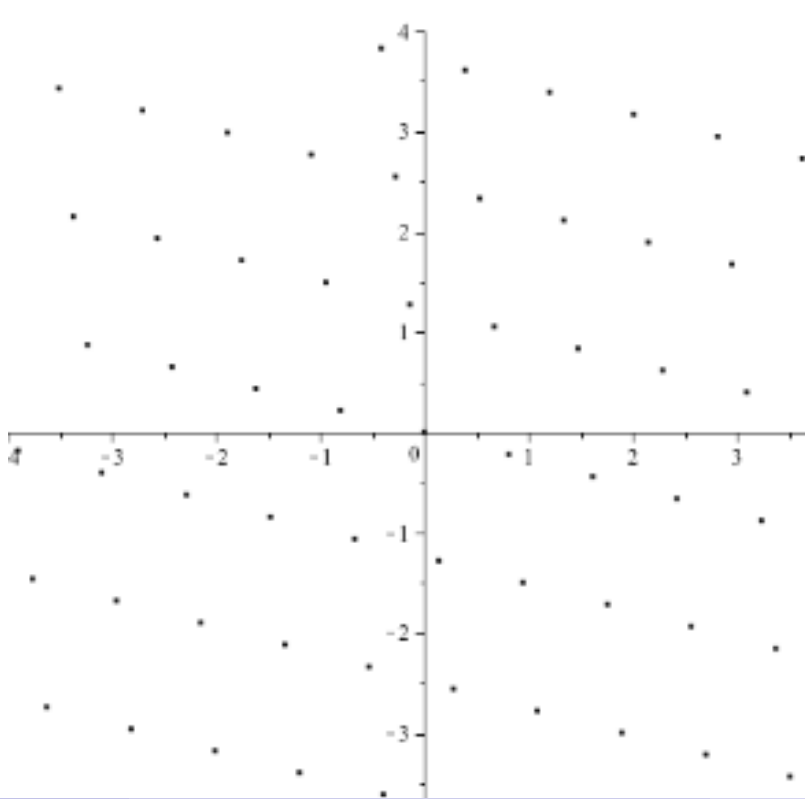
\includegraphics[width=0.5\textwidth]{images/section_6/lattice.png}
  \caption{Lattice in $\mathbb{R}^2$}
  \label{fig:lattice}
\end{figure}

\begin{defBox}{Rank}
    tThe rank of a lattice $\mathcal{L} \subset \mathbb{R}^n$, $rk(\mathcal{L})$ is the maximum number of linearly independent vectors in $\mathcal{L}$.\\
    The lattice is called \textbf{full-rank} or \textbf{complete} if rk($\mathcal{L}$) = $n$.\\
    If $\mathcal{L} \subset \mathbb{Z}^n$ is called \textbf{integer lattice}.
\end{defBox}

\noindent
\textbf{Example}
\begin{itemize}
    \item $\mathbb{Z}^5$  is a lattice
    \item $\{(x, 2x): x \in \mathbb{Z}\}$ is a lattice
    \item $\{(x, 2x): x \in \mathbb{R}\}$ is not a lattice, because it is not discrete.
    \item $\{(2x, x+1): x \in \mathbb{Z}\}$ is not a lattice, because it is not a subgroup of $\mathbb{R}^2$.
\end{itemize}

\subsection{Some properties of lattices}
The intersection of two lattices is a lattice of $\mathbb{R}^n$ is a lattice in $\mathbb{R}^n$.
\medskip

\noindent
If $\mathcal{L}$ is a lattice in $ c \in \mathbb{R}^x$ then
\begin{center}
    $\mathcal{L}c = \{cv: v \in \mathcal{L}\}$ is a lattice in $\mathbb{R}^n$.
\end{center}
This means that we procude a set by multiplying all elements of the lattice by a constant $c$
\medskip

\noindent
If $\mathcal{L}_1$ and $\mathcal{L}_2$ are lattices in $\mathbb{R}^n$ then
\begin{center}
    $\mathcal{L}_1 + \mathcal{L}_2 = \{v_1 + v_2: v_1 \in \mathcal{L}_1, v_2 \in \mathcal{L}_2\}$ is not in general a lattice in $\mathbb{R}^n$.
\end{center}
That because we can lost the discreteness property.
\bigskip

\begin{defBox}{Minimum Distance}
    GGiven a lattice $\mathcal{L}$, we define the minimum distance of $\mathcal{L}$, denoted by $\lambda(\mathcal{L})$, as the length of the shortest non-zero vector in $\mathcal{L}$
    \begin{center}
        $\lambda(\mathcal{L}) = \min\{\|v\|: v \in \mathcal{L} \setminus \{0\}\}$
    \end{center}
\end{defBox}
\noindent
Let us observe that $\lambda(\mathcal{L}) = \min\{\|v\|: v \in \mathcal{L} \setminus \{0\}\} = \min \{\|v - w\|: v, w \in \mathcal{L}, v \neq w\}$
\bigskip 

\noindent
A lattice $\mathcal{L}$ of $\mathbb{R}^n$ is generated by a finite number of linearly independent vectors.

\begin{defBox}{Basis}
    AA basis $\mathcal{B}$ of a lattice $\mathcal{L}$ is a set of linearly independent generators of $\mathcal{L}$.\\
    If $\mathcal{B} = \{b_1, b_2, \ldots, b_k\}$, then 
    \begin{center}
        $\mathcal{L} = \{\sum_{i=1}^k z_i b_i: z_i \in \mathbb{Z}\}$
    \end{center}
    where $k$ is the rank of $\mathcal{L}$.
\end{defBox}

\noindent
Each lattice can has many different bases.
\medskip

\noindent
A basis can be rapresented by a $r \times n$ matrix
\begin{center}
    $B = \begin{bmatrix}
    b_{1}\\
    b_{2}\\
    \vdots\\
    b_{r}
    \end{bmatrix}$
\end{center}
so that $\mathcal{L} = \{aB: a \in \mathbb{Z}^r\}$, where $a$ is a row vector of $\mathbb{Z}^r$.
\medskip

\noindent
If $B_1$ and $B_2$ are two bases of the same lattice $\mathcal{L}$, then there exists a unimodular matrix $U$ such that $B_1 = UB_2$.\\
\bigskip

\noindent
NOT EVERY set of r linearly independent vectors in a lattice is a basis.\\
This is true if the ”parallelepiped” it determines does not contain any point of $\mathcal{L}$ except its vertices.
\medskip

\noindent
A lattice can have a proper sublattice of the same rank.
\medskip

\noindent
A lattice does not admit in general an orthogonal basis

\subsubsection{Foundamental Domain}

\begin{defBox}{Foundamental Domain}
    LLet $\mathcal{L}$ be a lattice of rank $n$  with basis $\mathcal{B} = \{b_1, b_2, \ldots, b_n\}$. \\
    The foundamental domain is 
    \begin{center}
        $\mathcal{F}(\mathcal{B}) = \{\sum_{i=1}^n \alpha_i b_i: 0 \leq \alpha_i < 1\}$
    \end{center}
\end{defBox}

\begin{defBox}{Determinant}
    aGiven any basis $B$ (in matricial form) of a lattice $\mathcal{L}$, the determinant of $\mathcal{L}$, denoted det($\mathcal{L}$), is the volume of the fundamental domain. If $\mathcal{L}$ is full rank, then det($\mathcal{L}$) = $|\det B|$.
\end{defBox}

\noindent
\textbf{Remark:} The determinant is an invariant, i.e., it does not depend on the choice of the basis.
\medskip



\noindent
\textbf{Example:}\\
Consider the lattice generated by vectors $b_1 = (2, 1)$ and $b_2 = (1, -1)$, then the foundamental domain is the parallelogram determined by $b_1$ and $b_2$. [see Figure \ref{fig:foundamental_domain}]

\begin{figure}[h!]
  \centering
  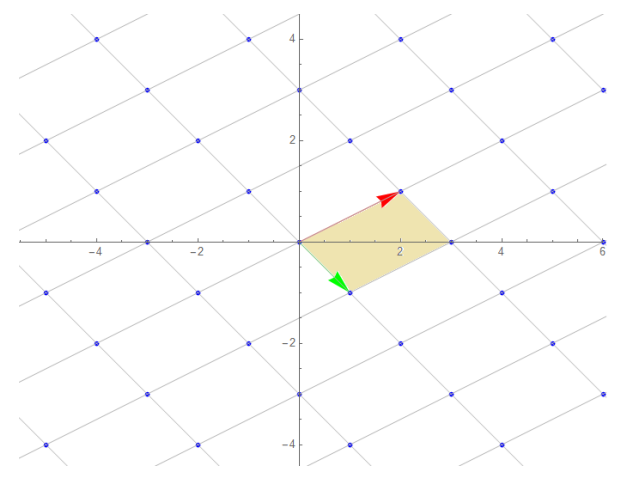
\includegraphics[width=0.75\textwidth]{images/section_6/foundamental_domain_1.png}
  \caption{Foundamental Domain}
  \label{fig:foundamental_domain}
\end{figure}

\noindent
Lattice generated by the vectors $b_1 = (1, 0, 0)$, $b_2 = (0, 1, 0)$ and $b_3 = (0, 0, 1)$ the foundamental domain is the cube determined by $b_1$, $b_2$ and $b_3$. [see Figure \ref{fig:foundamental_domain_cube}]

\begin{figure}[h!]
  \centering
  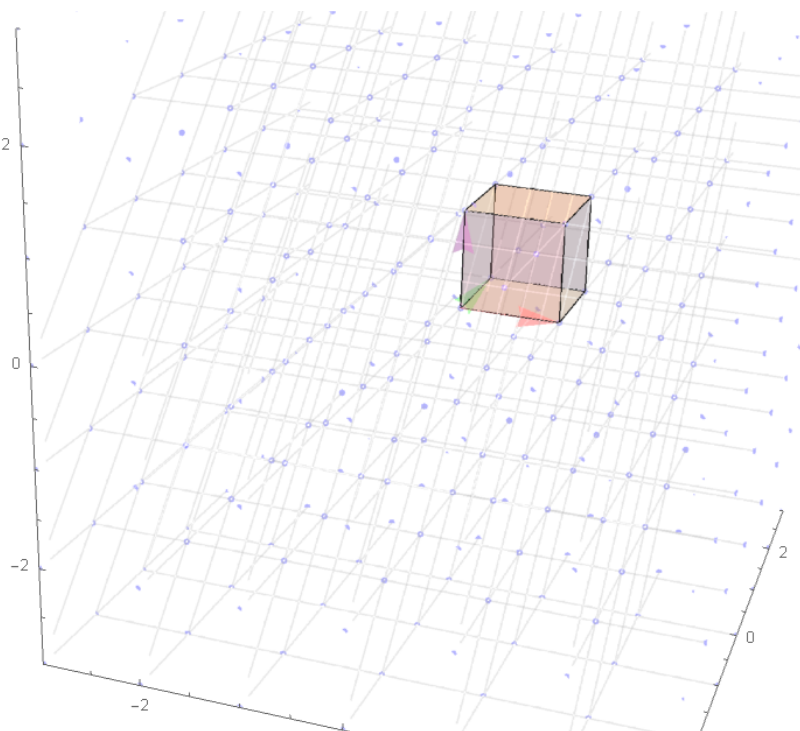
\includegraphics[width=0.75\textwidth]{images/section_6/foundamental_domain_3.png}
  \caption{Foundamental Domain in $\mathbb{R}^3$}
  \label{fig:foundamental_domain_cube}
\end{figure}

\newpage
\begin{propBox}{Minkowski's Bound}{}
    How long is a shortest nonzero vector in a lattice $\mathcal{L}$ of $\mathbb{R}^n$? The lattice $\mathcal{L}$ contains a nonzero vector $v$ satisfying:
    \begin{center}
        $\|v\| \leq \sqrt{n} \cdot (\det(\mathcal{L}))^{1/n}$
    \end{center}
\end{propBox}

\medskip

\begin{propBox}{}{}
    Let $\mathcal{L} \subset \mathbb{R}^n$ be a lattice of rank $n$, then $\forall v \in \mathbb{R}^n$ we have 
    \begin{center}
        $v = b + f$
    \end{center}
    for a unique $b \in \mathcal{L}$ and a unique $f \in \mathcal{F}$
\end{propBox}
\noindent
It is possible to provide a one-to-one correspondence between lattice and polynomials by means of the following mapping:
\begin{align*}
    \mathbb{Z}^n &\leftrightarrow \mathbb{Z}[x]_{< n}, (a_0, a_1, \ldots, a_{n-1}) \leftrightarrow a_0 + a_1 x + \ldots + a_{n-1} x^{n-1}
\end{align*}

\noindent
An ideal lattice is a lattice $\mathcal{L} \subseteq \mathbb{Z}^n$ such that is isomorphic to an ideal $I \subseteq \mathbb{Z}_{[X]}/(f(x))$ with $f(x) \in \mathbb{Z}[x]$ monic and irreducible polynomial


\subsection{Lattice Problems}
We are interested to define some computational problems related to lattices, that are the basis of the security of lattice-based cryptography.

\begin{defBox}{Shortest Vector Problem (SVP)}
    aGiven a lattice $\mathcal{L} \subseteq \mathbb{Z}^n$.\\
    The Shortest Vector Problem (SVP) is the problem of finding a non-zero vector $v \in \mathcal{L}$ such that $\|v\|= \min_{x \in \mathcal{L}, x \neq 0} \|v\| = \lambda(\mathcal{L})$. 
\end{defBox}

\begin{figure}[h!]
  \centering
  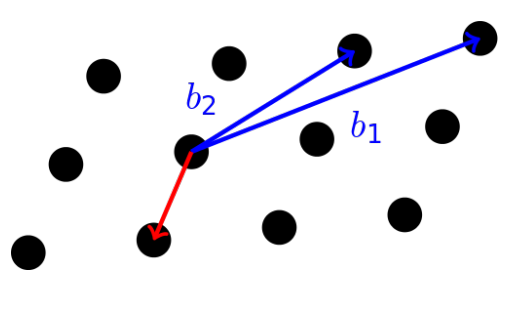
\includegraphics[width=0.4\textwidth]{images/section_6/SVP.png}
  \caption{Shortest Vector Problem}
  \label{fig:SVP}
\end{figure}

\begin{defBox}{Approximated SVP problem (SVP-$\gamma$)}
    TThe approximated SVP problem (SVP-$\gamma$) is the problem of finding a vector $v \in \mathcal{L}$ such that $\forall x \in \mathcal{L}$:
    \begin{center}
        $\|v \| \leq \gamma \min\|x\|$
    \end{center}
    where $\gamma \geq 1$ is an approximation factor.
\end{defBox}

\begin{defBox}{Closest Vector Problem (CVP)}
    gGiven a lattice $\mathcal{L} \subseteq \mathbb{Z}^n$ and a target vector $w \in \mathbb{R}^n$.\\
    The Closest Vector Problem (CVP) is the problem of finding a vector $v \in \mathcal{L}$ such that
    \begin{align*}
        \|v - w\| = \min_{x \in \mathcal{L}} \|x - w\|
    \end{align*}
\end{defBox}
\begin{figure}[h!]
  \centering
  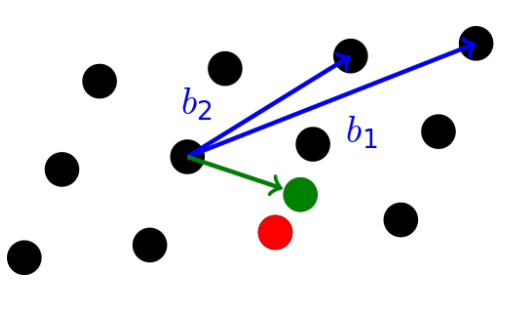
\includegraphics[width=0.4\textwidth]{images/section_6/CVP.png}
  \caption{Closest Vector Problem}
  \label{fig:CVP}
\end{figure}

\begin{defBox}{Approximated CVP problem (CVP-$\gamma$)}
    TThe approximated CVP problem (CVP-$\gamma$) is the problem of finding a vector $v \in \mathcal{L}$ such that $\forall x \in \mathcal{L}$:
    \begin{center}
        $\|v - w\| \leq \gamma \min\|x - w\|$
    \end{center}
    where $\gamma \geq 1$ is an approximation factor.
\end{defBox}

\noindent
SVP and CVP are computationally equivalent.\bigskip

\subsubsection*{Orthogonal basis case}
Both SVP and CVP are easy to solve if a lattice $\mathcal{L}$ of rank $n$ has an orthogonal basis $B = \{b_1, \ldots, b_n\}$ (considering a full rank lattice). Indeed, if $a_i \in \mathbb{Z}$, $t_i \in \mathbb{R}$ for all $i = 1, \ldots, n$ and $v \in \mathcal{L}$ we have:
\begin{align*}
    v &= \sum_{i=1}^n a_i b_i \implies \|v\|^2 = \sum_{i=1}^n a_i^2 \|b_i\|^2 \\
    w &= \sum_{i=1}^n t_i b_i \implies \|w - v\|^2 = \sum_{i=1}^n (a_i - t_i)^2 \|b_i\|^2
\end{align*}
Therefore to solve SVP we search the shortest nonzero vector in the set $\{\pm b_1, \ldots, \pm b_n\}$ and to solve CVP we take each $a_i$ as the integer closest to the corresponding $t_i$.


\subsubsection*{Lattices and Non-Orthogonal Bases}

Consider a lattice $L \subseteq \mathbb{R}^n$ of rank 2 whose basis is $\underline{b}_1 = (5, 1, 1)$ and $\underline{b}_2 = (4, 0, 1)$.
This is not an orthogonal basis, indeed:
\[ \underline{b}_1 \cdot \underline{b}_2 = 5 \cdot 4 + 1 \cdot 0 + 1 \cdot 1 = 21 \neq 0 \]

The lengths of these vectors are:
\[ ||\underline{b}_1|| = \sqrt{5^2 + 1^2 + 1^2} = \sqrt{27} \]
\[ ||\underline{b}_2|| = \sqrt{4^2 + 0^2 + 1^2} = \sqrt{17} \]

Let $\underline{v} = (v_1, v_2, \dots, v_n) \in \mathbb{R}^n$. Remember that the length of a vector is:
\[ ||\underline{v}|| = \sqrt{\underline{v} \cdot \underline{v}} = \sqrt{v_1^2 + v_2^2 + \dots + v_n^2} \]

\noindent
The shortest vector of $L$ is not, in this case, a vector of the basis. Indeed, for instance, $\underline{b}_1 - \underline{b}_2 \in L$ because it is a linear combination of $\underline{b}_1$ and $\underline{b}_2$ with integer coefficients. Since $\underline{b}_1 - \underline{b}_2 = (1, 1, 0)$, we have:
\[ ||\underline{b}_1 - \underline{b}_2|| = \sqrt{1^2 + 1^2 + 0^2} = \sqrt{2} \]
which is smaller than the length of $\underline{b}_1$ and $\underline{b}_2$.
\medskip

\noindent
Thus, in general, given a lattice $L$ and a non-orthogonal basis, the shortest vector is not necessarily a vector of the basis.

\subsubsection*{Lattices and Orthogonal Bases example}

Consider a lattice $L \subseteq \mathbb{R}^n$ of rank 2 whose basis is given by $\underline{b}_1$ and $\underline{b}_2$.\\ Suppose that this is an orthogonal basis, i.e., $\underline{b}_1 \cdot \underline{b}_2 = 0$.\\ 
Now, we see that the shortest vector of $L$ is a vector of the basis. 
\medskip

\noindent
A general vector $\underline{v}$ is a linear combination of $\underline{b}_1$ and $\underline{b}_2$ with integer coefficients: 
\[ \underline{v} = a_1\underline{b}_1 + a_2\underline{b}_2 \quad \text{with } a_1, a_2 \in \mathbb{Z} \]
\bigskip

\noindent
We consider the length of $\underline{v}$ squared (because it is more convenient):
\begin{align*}
||\underline{v}||^2 &= \underline{v} \cdot \underline{v} = (a_1\underline{b}_1 + a_2\underline{b}_2) \cdot (a_1\underline{b}_1 + a_2\underline{b}_2) \\
&= a_1^2(\underline{b}_1 \cdot \underline{b}_1) + a_2^2(\underline{b}_2 \cdot \underline{b}_2) + a_1a_2(\underline{b}_1 \cdot \underline{b}_2) + a_2a_1(\underline{b}_2 \cdot \underline{b}_1)
\end{align*}

\vspace{0.5cm}

\noindent
Since $a_1, a_2 \in \mathbb{Z}$ (and assuming $\underline{v} \neq \underline{0}$), we have $a_1^2 \ge 1$ or $a_2^2 \ge 1$, and consequently:
\[ ||\underline{v}||^2 \ge ||\underline{b}_1||^2 \quad \text{and} \quad ||\underline{v}||^2 \ge ||\underline{b}_2||^2 \]
Thus the shortest vector of $L$ can be $\underline{b}_1$ or $\underline{b}_2$.

\bigskip

\noindent
This holds in general. Consider $L \subseteq \mathbb{R}^n$ of rank $n$ with an orthogonal basis $\underline{b}_1, \dots, \underline{b}_n$.\\
For all $\underline{v} \in L$, we have $\underline{v} = a_1\underline{b}_1 + \dots + a_n\underline{b}_n$ with $a_i \in \mathbb{Z}$.

\begin{align*}
||\underline{v}||^2 &= \underline{v} \cdot \underline{v} = (a_1\underline{b}_1 + \dots + a_n\underline{b}_n) \cdot (a_1\underline{b}_1 + \dots + a_n\underline{b}_n) \\
&= a_1^2(\underline{b}_1 \cdot \underline{b}_1) + \dots + a_n^2(\underline{b}_n \cdot \underline{b}_n) = a_1^2||\underline{b}_1||^2 + \dots + a_n^2||\underline{b}_n||^2
\end{align*}

\noindent
Thus, if $L$ has an orthogonal basis, the shortest vector is a vector of the basis.

\subsubsection*{Closest Vector Problem}

A similar situation happens if, given $\underline{w} \in \mathbb{R}^n$, we search for the closest vector of $L$ to $\underline{w}$. In this case, we are searching for a vector $\underline{v} = a_1\underline{b}_1 + \dots + a_n\underline{b}_n \in L$ (with $a_i \in \mathbb{Z}$) that minimizes $||\underline{w} - \underline{v}||$, or equivalently $||\underline{w} - \underline{v}||^2$.
\medskip

\noindent
Since $\underline{b}_1, \dots, \underline{b}_n$ is a basis of $L$, it is also a basis of $\mathbb{R}^n$ (since they are linearly independent vectors), and:
\[ \underline{w} = t_1\underline{b}_1 + \dots + t_n\underline{b}_n \in \mathbb{R}^n \quad \text{with } t_i \in \mathbb{R} \]
\medskip

\noindent
We have $\underline{w} - \underline{v} = (t_1 - a_1)\underline{b}_1 + \dots + (t_n - a_n)\underline{b}_n$ and:

\begin{align*}
||\underline{w} - \underline{v}||^2 &= (\underline{w} - \underline{v}) \cdot (\underline{w} - \underline{v}) \\
&= \big((t_1 - a_1)\underline{b}_1 + \dots + (t_n - a_n)\underline{b}_n\big) \cdot \big((t_1 - a_1)\underline{b}_1 + \dots + (t_n - a_n)\underline{b}_n\big) \\
&= (t_1 - a_1)^2(\underline{b}_1 \cdot \underline{b}_1) + \dots + (t_n - a_n)^2(\underline{b}_n \cdot \underline{b}_n) \\
&= (t_1 - a_1)^2||\underline{b}_1||^2 + \dots + (t_n - a_n)^2||\underline{b}_n||^2
\end{align*}

\noindent
This quantity is minimized if and only if:
\begin{itemize}
    \item $a_1$ is the closest integer to $t_1$
    \item $a_2$ is the closest integer to $t_2$
    \item $\dots$
    \item $a_n$ is the closest integer to $t_n$
\end{itemize}

\subsubsection{Gram-Schmidt Orthogonalization}

Given a basis $\underline{v}_1, \dots, \underline{v}_n$ of $\mathbb{R}^n$, it transforms this into an orthogonal basis $\underline{u}_1, \dots, \underline{u}_n$ of $\mathbb{R}^n$:

\begin{align*}
\underline{u}_1 &= \underline{v}_1 \\
\underline{u}_2 &= \underline{v}_2 - \text{proj}_{\underline{u}_1}(\underline{v}_2)
\end{align*}

\noindent
Where $\text{proj}_{\underline{u}_1}(\underline{v}_2)$ is the orthogonal projection of $\underline{v}_2$ onto $\underline{u}_1$.
\bigskip

\noindent
Let us check that $\underline{u}_2$ is orthogonal to $\underline{u}_1$. Geometrically, this is the sum (the diagonal of the parallelogram) between the vectors $\underline{v}_2$ and $-\text{proj}_{\underline{u}_1}(\underline{v}_2)$.

\vspace{1 cm}

\noindent
If a lattice $\mathcal{L}$ has a basis $\mathcal{B} = \{b_1, \dots, b_n\}$ we searche for a good basis having shortest vector which are \textit{"as orthogonal as possible to each others"}.
\medskip

\noindent
We can not directly use the correspondig Gram-Schmidt basis $\mathcal{B}^*= \{b_1^{*}, \dots, b_n^{*}\}$: it is not a basis for $\mathcal{L}$, since the Gram-Schmidt process does not preserve the integrality of the coefficients.\\
However, $\mathcal{B}$ has a good property:
\begin{align*}
    det(\mathcal{L}) = \prod_{i=1}^n ||b_i^{*}||
\end{align*}

\noindent
(since the change of the basis matrix from $\mathcal{B}$ to $\mathcal{B}^*$ has determinat equal to 1) and we could use $\mathcal{B}^*$ in oreder to find a new basis for $\mathcal{L}$ as similar as possible to $\mathcal{B}^*$

\subsubsection{LLL algorithm}
In a lattice $\mathcal{L}$ of rank $n$ we have the \textbf{LLL algorithm} to reduce a basis $\mathcal{B} = \{v_1, \dots, v_n\}$ with associated Gram-Schmidt orthogonal basis $\mathcal{B}^* = \{v_1^{*}, \dots, v_n^{*}\}$ to a new basis with vectors as ortogonal as possible.\\
A basis is LLL-reduced if:

\begin{itemize}
    \item \textbf{Size condition}:
    \begin{align*}
    |\mu_{i,j}| = \frac{| v_i, v_j^{*} |}{||v_j^{*}||^2} \leq \frac{1}{2} \quad \text{for all } 1 \leq j < i \leq n 
    \end{align*}
    \item \textbf{Lovasz condition}:
    \begin{align*}
    ||v_i^{*}||^2 \geq \left(\frac{3}{4} - \mu_{i, j}^2\right) ||v_{i-1}^{*}||^2 \quad \text{for all } 2 \leq i \leq n
    \end{align*}
\end{itemize}

\begin{algorithm}
\caption{Lenstra--Lenstra--Lovász (LLL) Reduction Algorithm}
\begin{algorithmic}[1]

\Require Basis $\mathcal{B}=\{v_1,\dots,v_n\}$ of an $n$-dimensional lattice $L$
\Ensure LLL-reduced basis $\mathcal{B}_{LLL}=\{v_1,\dots,v_n\}$

\State $k \gets 2$
\State $v_1^* \gets v_1$

\While{$k \leq n$}

    \For{$j = k-1, k-2, \dots, 1$}
        \State $v_k \gets v_k - \lfloor \mu_{k,j} \rceil v_j$
        \Comment{Size Reduction}
    \EndFor

    \If{$\|v_k^*\|^2 \geq \left(\dfrac{3}{4} - \mu_{k,k-1}^2\right)\|v_{k-1}^*\|^2$}
        \State $k \gets k+1$
    \Else
        \State Swap $v_{k-1}$ and $v_k$
        \State $k \gets \max\{k-1,2\}$
        \Comment{Swap}
    \EndIf

\EndWhile

\State \Return $\mathcal{B}_{LLL}$

\end{algorithmic}
\end{algorithm}
\noindent
\textbf{Note:}
\[
\mu_{k,j} = \frac{\langle v_k, v_j^* \rangle}{\|v_j^*\|^2}
\]
where the vectors $v_1^*,\dots,v_k^*$ are computed using the Gram--Schmidt orthogonalization process.

\subsection{Learning With Errors -- LWE}

\begin{defBox}{Learning With Errors (LWE)}
 lLet $p$ be a prime and let $n \in \mathbb{N}^+$.\\
 Given a secret vector $s \in \mathbb{Z}_p^n$.\\
 The \textbf{LWE-distribution} $A_{s, \chi}$ is defined as:

 \begin{align*}
    A_{s, \chi} = \{(a, b) \in \mathbb{Z}_p^n \times \mathbb{Z}_p
 \end{align*}

\noindent
such that: 
\begin{itemize}
    \item $a$ is chosen uniformly at random from $\mathbb{Z}_p^n$ (vector of lenght a)
    \item $b$ is defined as:
    \begin{align*}
        b= s \cdot a + e \mod p = (\langle s, a \rangle + e) \mod p
    \end{align*}
    where $e$ is an error term chosen according to a distribution $\chi$ over $\mathbb{Z}_p$.\\
    So $b$ is a a scalar, dot product between $s$ and $a$ plus an error term
\end{itemize}
\end{defBox}
\medskip

\noindent
LWE are typcally hard problems. In particular:
\begin{itemize}
    \item \textbf{Search LWE:} The problem Search $LWE_{n, p, \chi, m}$ is to find $s \in \mathbb{Z}_p^n$ given $m$ pairs $(a, b) \in A_{s, \chi}$
    \item \textbf{Decision LWE:} The problem Decision $LWE_{n, p, \chi, m}$ is to say, given $m$ pairs $(a, b) \in A_{s, \chi}$ and $m$ pairs $(a, b)$ where $a$ if they belong to a LWE distribution with a same fixed $s$ or if they are randomly sampled from a uniform distribution in $\mathbb{Z}_p^n \times \mathbb{Z}_p$.
\end{itemize}
\noindent
The two problems are computationally equivalent.
\bigskip

\noindent
In cryptography, is more convinient to work with the Ring-LWE problem.

\begin{defBox}{Ring Learning With Errors (Ring-LWE)}
    lConsider a prime $p$ and $n \in \mathbb{N}^+$, define $R = \mathbb{Z}_p[X] / (X^n + 1)$.\\
    Let $s = s(X) \in R$ a fixed element called secret, wich is a polynomial of degree at most $n-1$ with coefficients in $\mathbb{Z}_p$.\\
    The \textbf{Ring-LWE distribution} $A_{s, \chi}$ is defined as:
    \begin{align*}        
        A_{s, \chi} = \{(a, b) \} \subseteq R \times R
    \end{align*}
    such that:
    \begin{itemize}
        \item $a = a(X)$ is chosen uniformly at random from $R$ 
        \item $b = b(X)$ is defined as:
            \begin{align*}
                b = (s \cdot a + e) \mod p
            \end{align*}
            where $e = e(X)$ is an error term chosen according to a distribution $\chi$ over $R$.
    \end{itemize}
\end{defBox}

\noindent
Also Ring-LWE is a hard problem:
\begin{itemize}
    \item \textbf{Search Ring-LWE:} The problem Search $RingLWE_{n, p, \chi, m}$ is to find $s \in R$ given $m$ pairs $(a, b) \in A_{s, \chi}$
    \item \textbf{Decision Ring-LWE:} The problem Decision $RingLWE_{n, p, \chi, m}$ is to say, given $m$ pairs $(a, b) \in A_{s, \chi}$ if they come from a Ring-LWE distribution with a same fixed $s$ or if they are randomly sampled from a uniform distribution in $R \times R$.
\end{itemize}
\section{Lattice-based cryptography}

\subsection{NTRU}
\begin{quotation}
    \textit{\textbf{Author's note:} As I already said, I strongly suggest to read the original paper, because the professor only gives a very high level overview of the scheme, and it's not possible to understand the details of the scheme without reading the original paper.\\
    Moreover, this paragraph will contain the fondumental parts needed aswer to a possible question in the exam.}
\end{quotation}

\subsubsection{Parameters and notation}
N,p,q integers with gcd(p,q)=1 and q>p.\\
(p and q are not necessarily prime and N$\neq$ pq)
\bigskip

\noindent
$R = \mathbb{Z}[X] / (X^N - 1)$ is the set of polynomials woth integer coefficients and degree at most N-1, they are all the possible reminders with respect to the division by $X^N - 1$.\\
The product in R will be denoted by $\circledast$
\bigskip

\noindent
$\mathcal{L}_f, \mathcal{L}_g, \mathcal{L}_\phi, \mathcal{L}_m$ are subsets of R.

\subsubsection*{Remark}
In R, $X^N = 1$ or equivalently $X^N \equiv 1 \mod (X^N - 1)$\\
Indeed, $X^N = 1 \cdot (X^N - 1) + 1$ and the reminder of the division of $X^N$ by $X^N - 1$ is 1.

\subsubsection*{Example}
Consider N=4 and F,G $\in$ R:
\begin{align*}
    &F= F_0 + F_1 X + F_2 X^2 + F_3 X^3 \\
    &\text{and}\\
    &G= G_0 + G_1 X + G_2 X^2 + G_3 X^3
\end{align*}

\noindent
We have:
\begin{align*}
    &F \circledast G = (F_0 + F_1 X + F_2 X^2 + F_3 X^3)\\ 
    &\circledast (G_0 + G_1 X + G_2 X^2 + G_3 X^3) = \\
    &= F_0 G_0 + F_0 G_1 X + F_0 G_2 X^2 + F_0 G_3 X^3 + F_1 \\
    &G_0 X + F_1 G_1 X^2 + F_1 G_2 X^3 + F_1 G_3 X^4 + \\
    &F_2 G_0 X^2 + F_2 G_1 X^3 + F_2 G_2 X^4 + F_2 G_3 X^5 + \\
    &F_3 G_0 X^3 + F_3 G_1 X^4 + F_3 G_2 X^5 + F_3 G_3 X^6=
\end{align*}
\noindent
But we have that $X^4 = 1$ so:

\begin{align*}
    = F_0 G_0 + F_1 G_3 + F_2 G_2 + F_3 G_1 + \\
    (F_0 G_1 + F_1 G_0 + F_2 G_3 + F_3 G_2) X + \\
    (F_0 G_2 + F_1 G_1 + F_2 G_0 + F_3 G_3) X^2 + \\
    (F_0 G_3 + F_1 G_2 + F_2 G_1 + F_3 G_0) X^3
\end{align*}

\subsubsection{Key Generation}
\begin{algorithm}
\begin{algorithmic}[1]

    \State Select $f \in \mathcal{L}_f \subseteq R$ s.t f is invertible in R$\mod$p and$\mod$q

    \State Select $g \in \mathcal{L}_g \subseteq R$

    \State Evaluate $F_p$ and $F_q$ the inverse of f in R$\mod$p and$\mod$q

    \State Evaluate $h \equiv F_q \circledast g \mod q$

\end{algorithmic}
\end{algorithm}

\subsubsection{Encryption}
Encryption of a message $m \in \mathcal{L}_m \subseteq R$.

\begin{algorithm}
\begin{algorithmic}[1]

    \State Select random $\phi \in \mathcal{L}_\phi$

    \State Evaluate $c \equiv p \cdot \phi \circledast h + m \mod q$

\end{algorithmic}
\end{algorithm}

\noindent
The one-way function is based on R-LWE

\newpage
\subsubsection*{Decryption}
\begin{algorithm}
\begin{algorithmic}[1] 

    \State Evaluate $a \equiv f \circledast c \mod q$

    \State Evaluate $F_q \circledast a \mod p \equiv m$
\end{algorithmic}
\end{algorithm}

\noindent
\textbf{Note}: In the reduction mod q (and mod p), we use the rapresentation in the inteval $[-\frac{q}{2}, \frac{q}{2}]$ (and $[-\frac{p}{2}, \frac{p}{2}]$) to avoid the wrap around effect.\\
For example, if we have $q=5$, we do not use {0,1,2,3,4} but we use $\{-2,-1,0,1,2\}$.
\medskip

\noindent
The centered representation modulo \(q\) does not prevent the modular reduction itself.\\ 
Rather, it allows us to interpret residues modulo \(q\) as small signed coefficients.\\ 
This is crucial in NTRU, because during decryption the intermediate coefficients are expected to be small.\\ 
If they remain inside the interval \([-\frac q2,\frac q2]\), then the centered reduction recovers their correct signed value.\\ 
If a coefficient exceeds this interval, a wrap around occurs and the value may be interpreted incorrectly, possibly causing decryption failure.
\medskip

\noindent
\textbf{E.g.} Let us consider \(q=11\). The standard representation modulo \(11\) is
\[
\{0,1,2,3,4,5,6,7,8,9,10\},
\]
whereas the centered representation is
\[
\{-5,-4,-3,-2,-1,0,1,2,3,4,5\}.
\]

\noindent
Therefore, the residues
\[
6,7,8,9,10
\]
are interpreted in the centered representation as
\[
6 \equiv -5 \pmod{11}, \qquad
7 \equiv -4 \pmod{11},
\]
\[
8 \equiv -3 \pmod{11}, \qquad
9 \equiv -2 \pmod{11}, \qquad
10 \equiv -1 \pmod{11}.
\]
\medskip

\noindent
For example, suppose that after an NTRU computation we obtain the following small coefficients:
\[
a=(-1,-4,0,2,-5).
\]
All these coefficients belong to the centered interval
\[
[-5,5].
\]

\noindent
However, if the coefficients are represented modulo \(11\) in the standard way, we obtain
\[
a \bmod 11 = (10,7,0,2,6),
\]
because
\[
-1 \equiv 10 \pmod{11}, \qquad
-4 \equiv 7 \pmod{11}, \qquad
-5 \equiv 6 \pmod{11}.
\]

\noindent
If we read the vector as
\[
(10,7,0,2,6),
\]
we may incorrectly interpret some coefficients as large positive values.  
Instead, using the centered representation, we recover
\[
(10,7,0,2,6)
\longrightarrow
(-1,-4,0,2,-5).
\]

\noindent
Thus, the centered representation allows us to correctly interpret residues modulo \(q\) as small signed coefficients, which is crucial in NTRU-based schemes.

\subsubsection*{Proof of correctness}
\begin{align*}
a \equiv f \circledast c \mod q \equiv f \circledast (p \cdot \phi \circledast h + m) \mod q \equiv p \cdot \phi \circledast g + f \circledast m \mod q
\end{align*}

\noindent
In the last equality we exploit the secret relation between the public and private keys. In particular the fact that $h \equiv F_q \circledast g \mod q$ is the trapdoor.
\medskip

\noindent
For appropriate choices of the parameters, we can ensure that the polynomial $a = p \cdot \phi \circledast g + f \circledast m$ is already reduced mod q, i.e., its coefficients are in the interval $[-\frac{q}{2}, \frac{q}{2}]$.\\
So that, the polynomial $a$ does not change if it is reduced mod q (we don't have the wrap around effect).
\medskip

\noindent
Then, when we evaluate $F_q \circledast a \mod p$, we have 
\begin{align*}
    F_q \circledast (p \cdot \phi \circledast g + f \circledast m) \mod p \equiv F_q \circledast f \circledast m \mod p \equiv m
\end{align*}
\noindent
In order to recover original message m, we need that the coefficients of m were already reduced mod p.

\subsubsection*{Remark}
Consider the ciphertext $c \equiv p \cdot \phi \circledast h + m \mod q$.\\
If we reduce $c \mod p$ we do not obtain m, because the polynomila $p \cdot \phi \circledast h + m$ has not the coeffincients  in the interval $[-\frac{p}{2}, \frac{p}{2}]$ (we have the wrap around effect), but they are larger, they wrap aroud mod q and consequently we do not find the original message m.\\
In general we gave the following situation:

\begin{itemize}
    \item $p \cdot \phi \circledast g + f \circledast m \mod q =\ p \cdot \phi \circledast g + f \circledast m \in \mathbb{Z}_{[X]}/(X^N - 1)$
    \item $p \cdot \phi \circledast h + m \mod q \neq p \cdot \phi \circledast h + m \in \mathbb{Z}_{[X]}/(X^N - 1)$
\end{itemize}

\noindent
It is clearly visible in the following example:

\subsubsection*{Example:}
Consider $N = 4$, $p = 7$ and $q = 19$.\\
Suppose 
\begin{align*}
    m = x^3 + x^2 + x + 1, \quad f = x^3 + x^2 + 1, \quad \phi \circledast g = 2x^3 + 2x^2+x+2
\end{align*}
\medskip

\noindent
Then we have:
\begin{align*}
    F_p = 4x^3+5x^2+5x+5, \quad F_q = 12x^3+13x^2+13x+13 \quad \text{and} \quad f\circledast m = 3x^3 + 3x^2 + 2x + 3
\end{align*}
\noindent
Now we compute:
\begin{align*}
    p \cdot \phi \circledast g + f \circledast m
    &= 14x^3 + 14x^2 + 7x + 14+3x^3 + 3x^2 + 3x + 3 \\
    &= 17x^3 + 17x^2 + 10x + 17
\end{align*}

\noindent
Which is the same polynomial after the reduction mod q:
\begin{align*}
    p \cdot \phi \circledast g + f \circledast m \mod q = 17x^3 + 17x^2 + 10x + 17
\end{align*}

\noindent
Thus, if we reduce the coefficients mod p, we get $f \circledast m= 17x^3 + 17x^2 + 10x + 17 \mod p = 3x^3 + 3x^2 + 3x + 3$
\vspace{1 cm}

\noindent
Let us see what happens to $c = p \cdot \phi \circledast g \circledast F_q + m:$
\begin{align*}
    \phi \circledast g \circledast F_q &= 89x^3 + 89x^2 + 89x + 90\\
    &\text{and}\\
    p \cdot \phi \circledast g \circledast F_q + m &= 623x^3 + 623x^2 + 623x + 630 + 3x^3 + 3x^2 + 3x + 3 = \\
    &\quad 626x^3 + 626x^2 + 626x + 633
\end{align*}

\noindent
And this polynomial changes after the reduction mod q:
\begin{align*}
    p \cdot \phi \circledast g \circledast F_q + m \mod q = 18x^3 + 18x^2 + 18x + 6
\end{align*}

\noindent
Thus, if we reduce the coefficients mod p, we DO NOT get m:
\begin{align*}
    18x^3 + 18x^2 + 18x + 6 \mod p = 4x^3 + 4x^2 + 4x + 6
\end{align*}
\medskip

\noindent
This is due to the fact that
\begin{align*}
    623 \equiv 0 \mod 7, \quad 630 \equiv 0 \mod 7
\end{align*}
\noindent
but
\begin{align*}
    &623 \equiv 15 \mod 19 \quad \text{and} \quad 15 \not\equiv 0 \mod 7\\
    &630 \equiv 3 \mod 19 \quad \text{and} \quad 3 \not\equiv 0 \mod 7
\end{align*} 
 
\subsubsection{Attacks against NTRU}

\subsubsection*{Brute force}
We want that  $|\mathcal{L}_f|, |\mathcal{L}_g|, |\mathcal{L}_\phi|$ are large enough to make the brute force attack infeasible.
\medskip

\noindent
Considering that $|\mathcal{L}_g| < |\mathcal{L}_f|$, let us evaluate the number of polynomials in $\mathcal{L}_g = \mathcal{L}(d_g, d_g)$ (remember that the polynomials in $\mathcal{L}_g$  are ternary polynomials with $d_g$ coefficients equal to 1, $d_g$ coefficients equal to -1 and the rest of the coefficients equal to 0)
\medskip

\noindent
Thus:
\begin{align*}
    |\mathcal{L}_g| &= \binom{N}{d_g} \cdot \binom{N-d_g}{d_g} \cdot 1 = \frac{N!}{d_g! \cancel{(N-d_g) !}} \cdot \frac{\cancel{(N-d_g)!}}{d_g! (N-2d_g)!} = \frac{N!}{d_g!^2 (N-2d_g)!}
\end{align*}
\vspace{0.5 cm}

\subsubsection*{Multiple Transmission Attack}
If we use the same publick key $h$ to encrypt several times the same message $m$, then an attacker can recover a sufficient number of coefficients of the random polynomial used during the encryption and then use \textbf{brute froce} to recover the original message.
\medskip

\noindent
Indeed, if we have
\begin{align*}
    &c_1 \equiv p \cdot \phi_1 h + m \mod q\\
    &c_2 \equiv p \cdot \phi_2 h + m \mod q\\
    &\vdots \\
    &c_k \equiv p \cdot \phi_k h + m \mod q
\end{align*}
\noindent
then the attacker can compute:
\begin{align*}
  c_1 - c_2 &\equiv p \cdot h (\phi_2 - \phi_1) \mod q \\
  \intertext{from which}
  \phi_2 - \phi_1 &\equiv p^{-1} h^{-1} (c_1 - c_2) \mod q
\end{align*}

\noindent
Thus, and attacker discovers $\phi_2 - \phi_1$ and similarly $\phi_3 - \phi_1, \phi_4 - \phi_1, \ldots, \phi_k - \phi_1$.\medskip

\noindent
Thanks to this polynomial can recover some coefficients of $\phi_1$ when he observe the coefficients $\neq 0,1,-1$ in the polynomials $\phi_2 - \phi_1, \phi_3 - \phi_1, \ldots, \phi_k - \phi_1$.

\subsubsection*{Example}
Remember that the polynomials $\phi_1, \phi_2, \ldots, \phi_k$ are ternary polynomials.\\
Suppose that $N = 8$ and
\begin{align*}
    &\phi_1 = x^5 + x^3 + 1\\
    &\phi_2 = x^7 + x^6 - x^4 + x^3 + x\\
    &\phi_3 = -x^5 + x^4 + x^2 -x
\end{align*}
\noindent
Then we have:
\begin{align*}
    &\phi_2 - \phi_1 = x^7 + x^6 - x^5 - x^4 + 2x^3 + x - 1\\
    &\phi_3 - \phi_1 = -2x^5 + x^4 + x^3 + x^2 - 2x + 1
\end{align*}

\noindent
If we only know these, we are sure that the coeffient of $x^3$ in $\phi_1$ must be -1 (otherwise it is impossible that $\phi_2 - \phi_1$ has a coefficient of 2 for $x^3$)\\
Similarly, we are sure that the coefficient of $x^5$ and $x$ in $\phi_1$ must be 1
\vspace{0.5 cm}

\subsubsection*{Lattice based attack}
Consider:
\begin{align*}
    &f = f_0 + f_1 x + \ldots + f_{N-1} x^{N-1} \\
    &g = g_0 + g_1 x + \ldots + g_{N-1} x^{N-1} \\
    &h = h_0 + h_1 x + \ldots + h_{N-1} x^{N-1}
\end{align*}

\noindent
and the corresponding vectors:
\begin{align*}
    &\vect{f} = (f_0, f_1, \ldots, f_{N-1}) \\
    &\vect{g} = (g_0, g_1, \ldots, g_{N-1}) \\
    &\vect{h} = (h_0, h_1, \ldots, h_{N-1})
\end{align*}

\noindent
The vector $(\alpha \vect{f}, \vect{g}) = (\alpha f_0, \alpha f_1, \ldots, \alpha f_{N-1}, g_0, g_1, \ldots, g_{N-1})$ is a short vector in the lattice of rank 2N whose basis is obtained exploiting the public key, for a convenient choice of $\alpha$.
\medskip

\subsubsection*{Example:}
Consider $N = 3$ and the lattice whose basis is given by the rows of the following 6x6 matrix:
\begin{align*}
    \begin{pmatrix}
        \alpha & 0 & 0 & h_0 & h_1 & h_2 \\
        0 & \alpha & 0 & h_2 & h_0 & h_1 \\
        0 & 0 & \alpha & h_1 & h_2 & h_0 \\
        0 & 0 & 0 & q & 0 & 0 \\
        0 & 0 & 0 & 0 & q & 0 \\
        0 & 0 & 0 & 0 & 0 & q
    \end{pmatrix}
\end{align*}

\noindent
we have that
\begin{align*}
    &f_0(\alpha, 0, 0, h_0, h_1, h_2) + f_1(0, \alpha, 0, h_2, h_0, h_1) + f_2(0, 0, \alpha, h_1, h_2, h_0)\\
    &= (\alpha f_0, \alpha f_1, \alpha f_2, f_0 h_0 + f_1 h_2 + f_2 h_1, f_0 h_1 + f_1 h_0 + f_2 h_2, f_0 h_2 + f_1 h_1 + f_2 h_0)
\end{align*}

\noindent
Note that the last three coordinates of this vector are equal to $g_0, g_1, g_2$ respectively.
\medskip

\noindent
Indeed, remember that
\begin{align*}
    h = F_q \circledast g \mod q \iff F_q \circledast h \equiv g \mod q
\end{align*}

\subsubsection{Size comparison}

\begin{table}[H]
\centering
\small
\renewcommand{\arraystretch}{1.35}
\resizebox{\textwidth}{!}{%
\begin{tabular}{|l|c|c|c|c|c|c|}
\hline
\rowcolor{gray!20}
& \textbf{PL} & \textbf{CT} & \textbf{RATIO} & \textbf{PK} & \textbf{SK} & \textbf{SECURITY} \\
\hline
\textbf{RSA} & 2048 & 2048 & 1 & 2048 & 2048 & 100 \\
\hline
\textbf{MCELIECE} & 524 & 1024 & 1.9 & $524 \cdot 1024$ & $524^2 + 524 \cdot 1024 + 8749$ & 65 \\
\hline
\textbf{NIED} & 284 & 500 & 1.76 & $500 \cdot 1024$ & $500^2+500 \cdot 1024 + 8749$ & 65 \\
\hline
\end{tabular}%
}
\caption{Size of plaintexts, ciphertexts and keys in bits.}
\end{table}

\noindent
\underline{NTRU, Case B}, $N=167$, $p=3$, $q=128$, $R = \mathbb{Z}[X]/(X^N-1)$
\medskip

\begin{itemize}
    \item \textbf{Plaintext:} $m \in R$ with coefficients reduced modulo p:\\ $\lceil \log_2 p \rceil \cdot N = 334 \text{ bits}$
    \item \textbf{Ciphertext:} $c \in R$ with coefficients reduced modulo q:\\ $\lceil \log_2 q \rceil \cdot N = 1169 \text{ bits}$
    \item \textbf{Ratio:} $\frac{1169}{334} = 3.5$
    \item \textbf{Public key:} $h \in R$ with coefficients reduced modulo q:\\ $\lceil \log_2 q \rceil \cdot N = 1169 \text{ bits}$
    \item \textbf{Private key:} $f, F_p \in R$ with coefficients reduced modulo p:\\ $2 \cdot \lceil \log_2 p \rceil \cdot N = 668 \text{ bits}$
\end{itemize}
\medskip

\noindent
\textbf{NOTE:} Remember that for representing an integer $N$, we need $\lceil \log_2 N \rceil$ bits.

\newpage
\subsection{Falcon}

\begin{quotation}
    \textit{\textbf{Author's note:} Also in this case, I strongly suggest to read the original paper.}
\end{quotation}

\noindent
Before describing Falcon scheme, we need to introduce some mathematical tools.\\
In particular it is necessary to introduce the concept of \textbf{Cyclotomic Polynomials}.

\subsubsection {Cyclotomic Polynomials}
The roots of the polynomial $X^N - 1$ are called N-th roots of unity and we denote them by $z_0, z_1, \ldots, z_{N-1}$.
\medskip

\noindent
We can explicitly write the complex number:
\begin{align*}
    z_k = e^{\frac{2 k\pi i}{N}} = \cos\left(\frac{2 k\pi}{N}\right) + i \sin\left(\frac{2 k\pi}{N}\right)
\end{align*}

\noindent
for $k = 0, 1, \ldots, N-1$.
\medskip

\noindent
Indeed $(z_k)^N = e^{2 k\pi i} = \cos 2k\pi + i \sin 2k\pi = 1$
\bigskip

\noindent
The set of ALL N-th roots of unity
\begin{align*}
    M_N = \{z_0, z_1, \ldots, z_{N-1}\}
\end{align*}
\noindent
is a \underline{cycling group} of order N and the generators of $M_N$ are called N-th primitive roots of unity.\\
\vspace{1 cm}

\noindent
Recalling that a cycling group of order N is isomorphic to the additive group $(\mathbb{Z}_N$, +), we have that:
\begin{itemize}
    \item Number of generators of $Z_N$ is $\varphi(N)$,\\ 
    so the number of generators of $M_N$ is $\varphi(N)$, i.e., the number of N-th primitive roots of unity is $\varphi(N)$
    \item The generator of $Z_N$  are all and only the integers $k$ comprime with N\\
    so  $z_k$ is a primitive root of unity if and only if $k$ is coprime with N (i.e., $\gcd(k, N) = 1$)
\end{itemize} 

\begin{defBox}{N-th Cyclotomic Polynomial}
    TThe N-th cyclotomic polynomial $\Psi_N(x)$ is the monic polynomial whose roots are all and only the N-th primitive roots of unity, i.e., $\Psi_N(x) = \prod_{k: \gcd(k, N) = 1} (x - z_k)$
\end{defBox}
\noindent
\textbf{Remark:} deg $\Psi_N(x) = \varphi(N)$
\vspace{0.5 cm}

\begin{propBox}{}{}
    \begin{align*}
        x^N - 1 = \prod_{d | N} \Psi_d(x)
    \end{align*}    
\end{propBox}

\noindent
\textbf{Idea of Proof:}
\begin{itemize}
    \item for all $d | N$, the roots of $\Psi_d(x)$ are also roots of $x^N - 1$ (because they are N-th roots of unity)\\
    Indeed, let $\alpha$ be a root of $\Psi_d(x)$, i.e., $\alpha^d = 1$ 
    \\
    then, $\alpha^N = \alpha^{md} = (\alpha^d)^m = 1^m = 1 (d \mid N \implies N = md)$
    \item It is also necessary to prove that
    \begin{align*}
        deg \prod_{d | N} \Psi_d(x) = N \iff \sum_{d | N} \varphi(d) = N
    \end{align*}
\end{itemize}

\noindent
Now, let us consider
\begin{align*}
    &N= 1, \quad, x-1 = \Psi_1(x)\\
    &N = 2, \quad x^2 - 1 = \Psi_1(x) \cdot \Psi_2(x) = (x-1)\Psi_2(x) \implies \boxed{\Psi_2(x) = x + 1}\\
    &N = 3, \quad x^3 - 1 = \Psi_1(x) \cdot \Psi_3(x) = (x-1)\Psi_3(x) \implies \boxed{\Psi_3(x) = x^2 + x + 1}\\
    &N = 4, \quad x^4 - 1 = \Psi_1(x) \cdot \Psi_2(x) \cdot \Psi_4(x) = (x-1)(x+1)\Psi_4(x) \implies \boxed{\Psi_4(x) = x^2+1}\\
    &\vdots\\
    &N = 8, \quad x^8 - 1 = \Psi_1(x) \cdot \Psi_2(x) \cdot \Psi_4(x) \cdot \Psi_8(x) = (x-1)(x+1)(x^2+1)\Psi_8(x)\\ 
    &\implies \boxed{\Psi_8(x) = x^4 + 1}\\
    &\vdots\\
    &N = 2^k, \quad x^{2^k} - 1 = \Psi_1(x) \cdot \Psi_2(x) \ldots \Psi_{2^k}(x) = (x-1)(x+1)(x^2+1)(x^4+1) \cdots (x^{2^{k-1}} + 1)\Psi_{2^k}(x)\\
    &\implies \boxed{\Psi_{2^k}(x) = x^{2^{k-1}} + 1}
\end{align*}

\subsubsection{Genealogy of Falcon}
Falcon is the product of many years of work, not only by the authors but also by others. This section explains how these works gradually led to Falcon as we know it.

\begin{figure}[htbp]
    \centering
    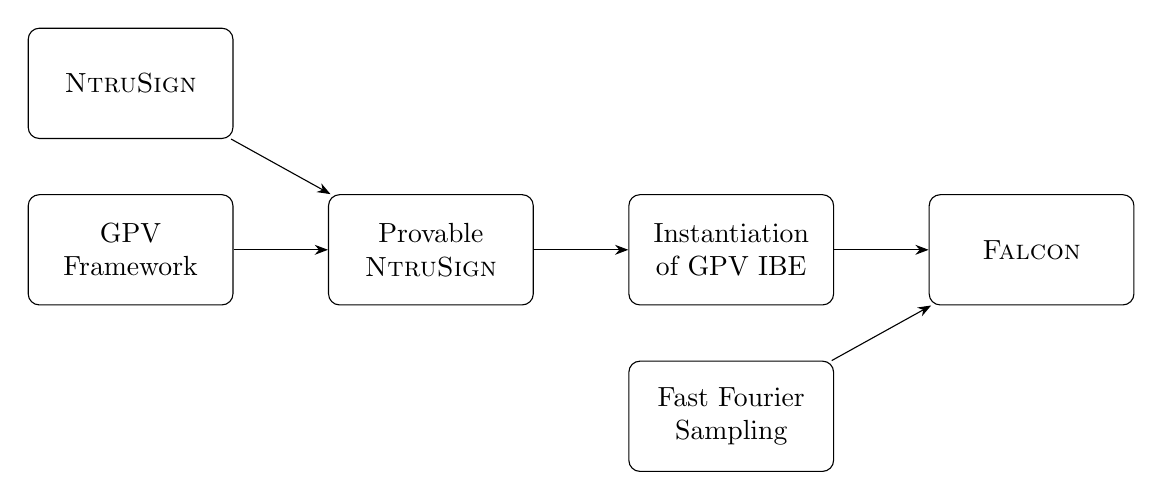
\begin{tikzpicture}[
        % Stile personalizzato per i rettangoli
        box/.style={
            draw, 
            rounded corners=4pt, 
            align=center, 
            minimum width=2.6cm, 
            minimum height=1.4cm,
            inner sep=6pt
        },
        % Stile delle frecce (Stealth assomiglia molto a quello dell'immagine)
        >=Stealth,
    ]

      
    \node[box] (gpv) {GPV\\ Framework};
    \node[box, right=1.2cm of gpv] (provable) {Provable\\ \textsc{NtruSign}};
    \node[box, right=1.2cm of provable] (inst) {Instantiation\\ of GPV IBE};
    \node[box, right=1.2cm of inst] (falcon) {\textsc{Falcon}};

    
    \node[box, above=0.7cm of gpv] (ntrusign) {\textsc{NtruSign}};
    \node[box, below=0.7cm of inst] (ffs) {Fast Fourier\\ Sampling};

    
    \draw[->] (gpv) -- (provable);
    \draw[->] (provable) -- (inst);
    \draw[->] (inst) -- (falcon);
    
    % Frecce diagonali
    \draw[->] (ntrusign) -- (provable);
    \draw[->] (ffs) -- (falcon);

    \end{tikzpicture}
    \caption{Genealogy of FALCON}
    \label{fig:falcon_genenealogy}
\end{figure}


\subsubsection{The Gentry-Peikert-Vaikuntanathan (GPV) Framework}
The GPV framework establishes a framework for constructing a secure lattice-based signature scheme.

\begin{itemize}
    \item The public key contain a full-rank matrix $A \in \mathbb{Z}_q^{n \times m}$ (where m > n) generating a q-ary lattice $\Lambda$
    
    \item The private key contains a matrix $B \in \mathbb{Z}_q^{m \times m}$  generating $\Lambda_q^\bot$\\
    where $\Lambda_q^\bot$ denotes the lattice ORTOGONAL to $\Lambda$: $\forall x \in \Lambda$ and $ y \in \lambda_q^\bot$, we have $\langle x, y \rangle \equiv 0 \mod q$ (where $\langle x, y \rangle$ is the standard inner product between the vectors $x$ and $y$)\\
    Equivalently, the rows of $A$ and $B$ are pairwise orthogonal: $B x A^t = 0$

    \item Given a message $m$, a signature of $m$ is a \underline{short vector} $s \in \mathbb{Z}^m$ such that $sA^t = H(m)$, where $H$ is a hash function ($\{0, 1\}* \to \mathbb{Z}_q^n$)
    
    \item Given $A$, verification of a signature $s$ for a message $m$ consists in checking that $sA^t = H(m)$ and that $s$ is short enough (i.e., $\|s\| \leq \beta$ for some parameter $\beta$)\\
    So it is straightforward 

    \item Computing a valid signature is more difficult.\\
    First, compute $c_0 \in \mathbb{Z}_q^m$ which verifies $c_0 A^t = H(m)$\\
    Even if $c_0$ is not short, we can simplify it with linear algebra.\\
    B is then used to compute a vector $v \in \Lambda_q^\bot$ close to $c_0$\\
    The difference $s = c_0 - v$ is a valid signature: indeed, $s A^t = c_0A^t - v A^t = c - 0 = H(m)$ and $s$ is short because $v$ is close to $c_0$.

\end{itemize}

\noindent
Note that $B$ is consider a good basis of $\Lambda_q^\bot$ if the vectors in $B$ are short and close to orthogonal.

\subsubsection{NTRU lattice}
As already said, Falcon exploits the NTRU lattice.
\medskip

\noindent
Let $\phi = x^n +1$ for $n = 2^k$.\\
A set of NTRU secret consist in 4 polynomials $f, g, F, G \in \mathbb{Z}[X]/(\phi)$ such that 

\begin{align*}
    fG - gF = q \mod \phi  \text{ (NTRU equation)}.
\end{align*}

\noindent
Provided that $f$ is invertible modulo $q$, we can define the public key as $h \gets g  \cdot f^{-1} \mod q$ and the private key as the tuple $(f, g, F, G)$.\\
Indeed, one can check that the matrices 
\begin{align*}
    \left[ \begin{array}{c|c}
        1 & h \\
        \hline
        0 & q
    \end{array} \right] \quad \text{and} \quad \left[ \begin{array}{c|c}
        f & g \\
        \hline
        F & G
    \end{array} \right]
\end{align*}

\noindent
generate the same lattice, but the first one contains two large polynomials ($h$ and $q$) while the second one contains four small polynomials.
\medskip

\noindent
If $f, g$ are generated with enough entropy, then $h$ will look pseudorandom. However in practice, even when $f, g$ are quite small, it remains hard to find small polynomials $f', g'$ such that $h = g' \cdot (f')^{-1} \mod q$. The hardness of this problem constitutes the \textbf{NTRU assumption}.

\subsubsection*{Instantiation with the GPV framework}
We now instantiate GPV.

\begin{itemize}
    \item The public basis is the matrix $A = [1 | h^*]$ where $h^*$ is the vector of the coefficients of $h$ (i.e., if $h = h_0 + h_1 x + \ldots + h_{n-1} x^{n-1}$, then $h^* = (h_0, h_1, \ldots, h_{n-1})$)
    
    \item The secret basis is the matrix $B = \left[ \begin{array}{c|c}
        g & -f \\
        \hline
        G & -F
    \end{array} \right]$
    One can check that $A$ and $B$ are indeed orthogonal:$B x A^* = 0 \mod q$ 

    \item The signature of a message of a message $m$ is composed by two polynomials $s_1, s_2$ such that $s_1 + s_2 h = H(m|r)$, where $r$ is a random salt.\\
    Note that, since $s_1$ is completely determined by $m, r, s_2$, it is sufficient to store only $(s_2, r)$ in the signature.
\end{itemize}

\noindent
\textbf{Computation:}\\
$A* = [1 | h]$

\begin{align*}
    B \cdot A^* = \left[ \begin{array}{c|c}
        g & -f \\
        \hline
        G & -F
    \end{array} \right] \cdot \left[ \begin{array}{c}
        1 \\
        \hline
        h
    \end{array} \right] =  \left[ \begin{array}{c}
        g - f h \\
        \hline
        G - F h
    \end{array} \right] =  \left[ \begin{array}{c}
        g - g \\
        \hline
        G - G
    \end{array} \right] = 0
\end{align*}    

\noindent
Since the public key is defined as
\[
h \equiv g f^{-1} \pmod q,
\]
we have
\[
fh \equiv f g f^{-1} \equiv g \pmod q.
\]

\noindent
Moreover, from the NTRU equation
\[
fG-gF \equiv 0 \pmod q,
\]
we obtain
\[
fG \equiv gF \pmod q.
\]

\noindent
Multiplying both sides by \(f^{-1}\), we get
\[
G \equiv Fgf^{-1} \equiv Fh \pmod q.
\]

\noindent
Therefore, we get 0 as expected

\subsubsection{Fast Fourier Sampling}
The authors exploit the Fast Fourier Transform (FFT) to speed up the sampling of the signature.
\medskip

\noindent
The idea is to represent the polynomials in the evaluation form, i.e, as vectors of the evaluations of the polynomials at the N-th roots of unity.\\
So instead of representing a polynomial $a = a_0 + a_1 x + \ldots + a_{n-1} x^{n-1}$ as the vector of its coefficients $(a_0, a_1, \ldots, a_{n-1})$, we represent it as the vector of its evaluations at the N-th roots of unity $(a(z_0), a(z_1), \ldots, a(z_{n-1}))$. where $z_0, z_1, \ldots, z_{n-1}$ are the N-th roots of unity (complex numbers).


\subsubsection{Falcon algorithms}

\begin{quotation}
    \textit{\textbf{Author's note:} This section is made to simplify the description of the main algorithms. For a more detailed description, I suggest to read the original paper.}
\end{quotation}
\bigskip

\noindent
Remember that Falcon fix:
\begin{align*}
    q, n \in \mathbb{Z}, \text{ where } n = 2^k\\
    \phi = x^n + 1\\
    R = \mathbb{Z}[X]/(\phi)
\end{align*}

\subsubsection*{Key Generation}
\begin{algorithm}
\begin{algorithmic}[1]
    \State Sample $f, g \in R$ s.t $(||f||, ||g||) < 1.17 \sqrt{q}$

    \State Compute $F, G \in R$ s.t. $fG - gF  = q$ (NTRU equation)

    \State Define B as the matrix $\left[ \begin{array}{c|c}
        g & -f \\
        \hline
        G & -F
    \end{array} \right]$ good basis of lattice $\Lambda_q^\bot$.
    Then we compute $\hat{B}$ applying the FFT to each element of $B$ 

    \State Compute $h = g \cdot f^{-1} \mod q$ and define $A = [1 | h^*]$ where $h^*$ is the vector of the coefficients of $h$

    \State Return $pk = h$ and $sk = (f, g, F, G)$
    
\end{algorithmic}
\end{algorithm}

\noindent
In order to compute $F, G$  we can reduce the problem over the integers, exploiting two operators:

\begin{itemize}
    \item \textbf{Split:} 
        \begin{align*}
            A(x) = a_0 + a_1 x + \ldots + a_{n-1} x^{n-1} \xrightarrow{\text{Split}} (A_0(x), A_1(x))
        \end{align*}
        where $A_0(x)$ contains the powers of $x$ with even exponent and $A_1(x)$ contains the powers of $x$ with odd exponent.\\
        For example, if $A(x) = 3 + 2x + 5x^2 + 7x^3$, then $A_0(x) = 3 + 5x$ and $A_1(x) = 2 + 7x$\\
        Iterating the split operator, we can split a polynomial in $R$ into $n$ polynomials of degree 0, i.e., into $n$ integers.

    \item \textbf{Merge:}
        \begin{align*}
            (A_0(x), A_1(x)) \xrightarrow{\text{Merge}} A(x) = A_0(x^2) + x A_1(x^2)
        \end{align*}
        For example, if $A_0(x) = 3 + 5x$ and $A_1(x) = 2 + 7x$, then $A(x) = A_0(x^2) + x A_1(x^2) = 3 + 5x^2 + 2x + 7x^3 = 3 +        2x + 5x^2 + 7x^3$
\end{itemize}

\subsubsection*{Signature}

\begin{algorithm}
\begin{algorithmic}[1]

    \State Compute $H(r \mid m) = c$ where $c \in R$

    \State Observe that
    \[
        (\vect{c},\vect{0})A^* = c
    \]
    where
    \[
        A^* = [1 \mid h]
    \]

    \State Compute
    \[
        t = (\vect{c},\vect{0})B^{-1}
    \]
    such that
    \[
        \vect{t}B = (\vect{c},\vect{0})
    \]

    \State Find a lattice vector $z$ generated by $B$ close to $t$
    
    \State Define
    \[
        \vect{s} = (s_1,s_2) = (\vect{t}-\vect{z})\hat{B}
    \]
    where $\hat{B}$ is the FFT representation of $B$

    \State Observe that $\vect{s}$ is short and satisfies:
    \[
        \vect{s}A^*
        =
        (\vect{t}-\vect{z})\hat{B}A^*
    \]

    \State Since the rows of $B$ are orthogonal to $A^*$, we have:
    \[
        z\hat{B}A^* = 0
    \]

    \State Therefore:
    \[
        \vect{s}A^*
        =
        t\hat{B}A^*
        =
        (\vect{c},\vect{0})B^{-1}\hat{B}A^*
        =
        (\vect{c},\vect{0})A^*
        =
        \vect{c}
    \]

    \State Return the signature $(s_2,r)$

\end{algorithmic}
\end{algorithm}

\noindent
The main computational challenge is finding a lattice vector $z$ close to $t$.\\
Falcon solves this problem efficiently exploiting the recursive tree structure of $\hat{B}$ together with FFT representations, reducing the problem to operations over the integers through a divide-and-conquer approach.\\
Moreover, Gaussian sampling is used in order to randomize the signatures and prevent leakage of information about the private basis.
\newpage

\subsubsection*{Verification}
\begin{algorithm}
\begin{algorithmic}[1]
    \State Check that $||s_2|| \leq \beta$ for some parameter $\beta$
    \State Compute $s_1 + s_2 h = c \mod q$ where $c = H(m|r)$
    \State Return 1 if $s_1 + s_2 h = c \mod q$, 0 otherwise
\end{algorithmic}
\end{algorithm}

\subsubsection{Comparison}
\begin{table}[H]
\centering
\small
\renewcommand{\arraystretch}{1.35}
\begin{tabular}{|c|c|c|c|c|}
\hline
\rowcolor{gray!20}
\textbf{Scheme} & \textbf{Security Level} & \textbf{Public Key} & \textbf{Secret Key} & \textbf{Signature Size} \\
\hline

RSA-15360 & $\approx 256$ bits & $\approx 2$ KB & $\approx 5$ KB & $\approx 2$ KB \\
\hline

ECDSA-521 & $\approx 256$ bits & $\approx 0.1$ KB & $\approx 0.04$ KB & $\approx 0.1$ KB \\
\hline

Classic McEliece & $\approx 256$ bits & $\approx 1.2$ MB & $\approx 14$ KB & N/A \\
\hline

HQC & $\approx 256$ bits & $\approx 7$ KB & $\approx 7$ KB & N/A \\
\hline

Falcon-1024 & $\approx 256$ bits & $\approx 1.8$ KB & $\approx 2.3$ KB & $\approx 1.3$ KB \\
\hline

\end{tabular}
\caption{Approximate comparison of key and signature sizes for classical and post-quantum cryptographic schemes at the 256-bit security level.}
\label{tab:pqc_comparison}
\end{table}

\noindent
In Falcon, signatures are represented by short polynomials sampled according to a discrete Gaussian distribution.\\
Although a coefficient in $\mathbb{Z}_q$ would normally require approximately $\log_2(q)$ bits, most sampled coefficients are concentrated around zero.\\
Indeed, for a Gaussian distribution with mean $\mu$ and standard deviation $\sigma$, approximately $99.7\%$ of the values lie in the interval
\[
[\mu - 3\sigma,\mu + 3\sigma].
\]

\noindent
Therefore, Falcon can compress signatures efficiently by encoding mainly small coefficients rather than arbitrary elements modulo $q$.\\
This allows Falcon to achieve significantly smaller signatures compared to many other post-quantum schemes.

\section{Introduction to Multivariate Systems}
NIST opened a call for signature-scheme proposals. The competition is currently in its third round, and nine finalists have been selected.\\
Four of the nine finalists are based on multivariate systems:
\begin{itemize}
    \item MAYO
    \item UOV
    \item QR-UOV
    \item SNOVA
\end{itemize}

\subsubsection*{Recap: classes of complexity}
\begin{defBox}{P problems}
    TThe class \textbf{P} is the class of decision problems that are decidable in polynomial time by a deterministic Turing machine.
\end{defBox}

\noindent
In other words, a problem is in \textbf{P} if there exists an algorithm that can solve any instance of the problem in time that is polynomial with respect to the size of the input.\\

\begin{defBox}{NP problems}
    TThe class \textbf{NP} is the class of decision problems for which a given solution can be verified in polynomial time by a deterministic Turing machine.
\end{defBox}


\noindent
In other words, a problem is in \textbf{NP} if there exists an algorithm that can verify whether a given solution to the problem is correct in polynomial time with respect to the size of the input.\\

\begin{defBox}{NP-hard problems}
    aA problem is \textbf{NP-hard} if every problem in NP can be reduced to it in polynomial time.
\end{defBox}
\noindent
In other words, a problem is \textbf{NP-hard} if it is at least as hard as the hardest problems in NP. If a problem is NP-hard, it means that if we could solve it efficiently, we could solve all problems in NP efficiently as well.\\

\begin{defBox}{NP-complete problems}
    aA problem is \textbf{NP-complete} if it is both in NP and NP-hard.
\end{defBox}
\noindent
In other words, a problem is \textbf{NP-complete} if it is in NP and is as hard as the hardest problems in NP. If a problem is NP-complete, it means that if we could solve it efficiently, we could solve all problems in NP efficiently as well.
\bigskip

\noindent
The question of whether \textbf{P} = \textbf{NP} is one of the most important open problems in computer science. \\
It asks whether every problem that can be verified in polynomial time can also be solved in polynomial time. If \textbf{P} = \textbf{NP}, it would mean that all problems in NP can be solved efficiently, which would have profound implications for fields such as cryptography, optimization, and algorithm design. However, most experts believe that \textbf{P} $\neq$ \textbf{NP}, meaning that there are problems in NP that cannot be solved efficiently, even though their solutions can be verified efficiently.
\vspace{0.5 cm}

\noindent
Many post-quantum cryptographic schemes are based on NP-complete problems.\\
Under specific assumptions, Multivariate Polynomial Problems are NP-complete.

\subsection{Multivariate Polynomial Problems}
\begin{defBox}{Multivariate Polynomial Problem (MPP)}
    aGiven $m$ polynomials of degree $d \geq 2$, $p_1, \ldots, p_m \in \mathbb{F}_q[x_1, \ldots, x_n]$, find a solution of the system
    \[
        \left\{
        \begin{aligned}
            &p_1(x_1, \ldots, x_n) &= 0\\
            &p_2(x_1, \ldots, x_n) &= 0\\
            &\vdots\\
            &p_m(x_1, \ldots, x_n) &= 0
        \end{aligned}
        \right.
    \]
\end{defBox}
\noindent
In other words, the Multivariate Polynomial Problem (MPP) asks us to find a solution to a system composed of $m$ equations and $n$ unknowns.
\medskip

\noindent
The particular case of the MPP where $m = 2$ and polynomials are of degree 2 is called the \textbf{MQ problem} (Multivariate Quadratic Problem).\\
The MQ problem is NP-complete, and it is the most common case in multivariate cryptography.
\medskip

\noindent
The choice to have only quadratic polynomials is motivated by the fact that solving a system of higher degree polynomials increase th complexity only polynomially.

\subsection{Overview of Multivariate Cryptography}
In multivariate cryptography, we can construcut both signature schemes and encryption schemes by exploiting the following idea:
\medskip

\noindent
Given the evaluation map

\begin{align*}
    P: \mathbb{F}_q^n &\to \mathbb{F}_q^m\\
    x= (x_1, \ldots, x_n) &\mapsto (p_1(x), \ldots, p_m(x))
\end{align*}

\noindent
where $p_1, \ldots, p_m$\\
and given $y = (y_1, \ldots, y_m) $, the difficult problem is to find a preimage $P^{-1}(y)$, i.e. a solution of the system, i.e an n-tuple $x = (x_1, \ldots, x_n)$ such that
\begin{align*}
    P(x_1, \ldots, x_n)= (y_1, \ldots, y_m)
\end{align*}

\noindent
\textbf{Note:}\\
Let $f : A \to B$ be a function and $y \in B$.
A preimage of $y$ is an element $x \in A$ such that $f(x) = y$.
\vspace*{2em}

\noindent
When we use this idea to construct a signature scheme we prefer to have $n < m$, so that the system is underdetermined and has many solutions.\\
On the other hand, when we use this idea to construct an encryption scheme we prefer to have $n = m$, so that the system is square and has a unique solution.

\subsubsection{Central Map}
The general framework consists of a secret fuction called central map, that is
\begin{align*}
    F: \mathbb{F}_q^n &\to \mathbb{F}_q^m\\
    x= (x_1, \ldots, x_n) &\mapsto (f_1(x_1, \ldots, x_n), \ldots, f_m(x_1, \ldots, x_n))
\end{align*}

\noindent
and two secret affine transformations $S: \mathbb{F}_q^n \to \mathbb{F}_q^n$ and $T: \mathbb{F}_q^m \to \mathbb{F}_q^m$.\\
These two functions can also be rapresented as matrices, and we can write $S \in \mathbb{F}_q^{n \times n}$ and $T \in \mathbb{F}_q^{m \times m}$.\\
\bigskip

\noindent
The trapdoor is the information of the internal structure of the map $P$, called the public map, where $P$ is defined as:
\begin{align*}
    P = S \circ F \circ T
\end{align*}
\noindent
That means starting from $x \in \mathbb{F}_q^n$, we first apply the transformation $T$ to get $T(x)$, then we apply the central map $F$ to get $F(T(x))$, and finally we apply the transformation $S$ to get $P(x) = S(F(T(x)))$.\\

\begin{figure}[ht]
\centering
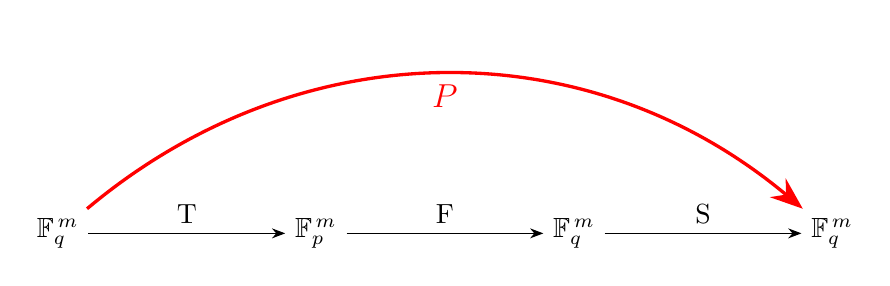
\begin{tikzpicture}[>=Stealth, node distance=2.5cm, auto]
    \node (A) {${\mathbb{F}}_q^{\,m}$};
    \node (B) [right=of A] {${\mathbb{F}}_p^{\,m}$};
    \node (C) [right=of B] {${\mathbb{F}}_q^{\,m}$};
    \node (D) [right=of C] {${\mathbb{F}}_q^{\,m}$};

    \draw[->] (A) -- node[above]{T} (B);
    \draw[->] (B) -- node[above]{F} (C);
    \draw[->] (C) -- node[above]{S} (D);
    \draw[->, very thick, red, bend left=40, >={Stealth[scale=1.4]}] (A) to node[midway, below]{\large $P$} (D);
\end{tikzpicture}
\end{figure}

\noindent
The main and most used trapdoors for multivariate cryptographic schemes are:
\begin{itemize}
    \item Hidden Field Equations (HFE): the trapdoor information is that the public system of
    quadratic polynomials arises from a single (secret) univariate polynomial over a finite field
    extension $\mathbb{F}_{q^m}$.
    \item Oil and Vinegar (OV): the trapdoor information is that the system of polynomials vanishes on a small (secret) subspace, called the Oil subspace
\end{itemize}

\subsubsection*{Example of MQ problem}
Let us consider the system of 4 multivariate polynomials in $\mathbb{F}_2[x_1, x_2, x_3]$.
\begin{equation*}
    \left\{
    \begin{array}{l}
        x_1x_3 + x_2x_3 + x_1 + x_2 + x_3 = 0,\\
        x_2x_3 + x_2 + 1 = 0,\\
        x_1x_2 + x_1x_3 + x_2 + x_3 = 0,\\
        x_1x_2 + x_2x_3 + x_1 = 0.
    \end{array}
    \right.
\end{equation*}

\noindent
We can ignore the fact that the system is quadratic and solve it as a linear system by introducing new variables $y_i$ as:
\begin{align*}
    y_1 &= x_1, y_2 = x_2, y_3 = x_3, \\
    y_4 &= x_1x_2, y_5 = x_1x_3, y_6 = x_2x_3.
\end{align*}
The system can be rewritten as:
\begin{equation*}
    \left\{
    \begin{array}{l}
       y_1 + y_3 + y_5 + y_6 = 0, \\
       y_2 + y_6 + 1 = 0, \\
       y_2 + y_3 + y_4 + y_5 = 0, \\
       y_1 + y_4 + y_6 = 0.
    \end{array}
    \right.
\end{equation*}
\noindent
The complete matrix of the system is:
\[
\left(
\begin{array}{cccccc|c}
1 & 0 & 1 & 0 & 1 & 1 & 0 \\
0 & 1 & 0 & 0 & 0 & 1 & 1 \\
0 & 1 & 1 & 1 & 1 & 0 & 0 \\
1 & 0 & 0 & 1 & 0 & 1 & 0
\end{array}
\right)
\longrightarrow
\left(
\begin{array}{cccccc|c}
1 & 0 & 0 & 1 & 0 & 1 & 0 \\
0 & 1 & 0 & 0 & 0 & 1 & 1 \\
0 & 0 & 1 & 1 & 1 & 1 & 1 \\
0 & 0 & 0 & 0 & 0 & 0 & 0
\end{array}
\right)
\]

\noindent
so that reduced system is:
\begin{equation*}
    \left\{
    \begin{array}{l}
       y_1 =  y_4 + y_6, \\
       y_2 = y_6 + 1, \\
       y_3 = y_4 + y_5 + y_6 + 1, \\
\end{array}
    \right.
\end{equation*}
\vspace{0.4 cm}

\noindent
The 8 solutions $(y_1,y_2,y_3,y_4,y_5,y_6)$ of the linearized system are:
\[
\begin{array}{cccc}
(0,1,1,0,0,0), &
(1,0,0,0,0,1), &
(0,1,0,0,1,0), &
(1,0,1,0,1,1), \\[4pt]
(1,1,0,1,0,0), &
(0,0,1,1,0,1), &
(1,1,1,1,1,0), &
(0,0,0,1,1,1).
\end{array}
\]
\medskip

\noindent
The problem is that they are not all solutions of the original system in the variables
$x_1,x_2,x_3$.\\
The only actual solution is
\[
(1,1,0,1,0,0).
\]
\bigskip

\noindent
For example, the solution
\[
(y_1,y_2,y_3,y_4,y_5,y_6)=(0,1,1,0,0,0)
\]
corresponds to:
\[
x_2=1,\qquad x_3=1,\qquad x_2x_3=0,
\]
which is clearly not possible.

\bigskip

\noindent
The step from the solution of the linearized system to the solution of the actual system gives rise, in general, to an exponential number of parasitic solutions.

\subsubsection{Solving Multivariate Systems}
In a quadratic system over the variables \(x_1,\dots,x_n\), linearization introduces one new variable \(y_i\) for each quadratic monomial. The number of quadratic monomials in \(n\) variables is
\[
t=\frac{n(n+1)}{2}.
\]

\noindent
More generally, the number of monomials of degree \(d\) in \(n\) variables is
\[
\binom{n+d-1}{d}.
\]

\noindent
After linearization, the original quadratic system is transformed into a linear system in \(t\) variables. If the system contains \(r\) linearly independent equations, then by linear algebra the number of free variables is
\[
t-r.
\]

\noindent
Over a finite field \(\mathbb F_q\), each free variable can assume \(q\) possible values. Therefore, the linearized system has
\[
q^{t-r}
\]
solutions.
\medskip

\noindent
In the quadratic case, since
\[
t=\frac{n(n+1)}{2},
\]
the number of solutions of the linearized system is
\[
q^{\frac{n(n+1)}{2}-r}.
\]

\noindent
The key issue is that many of these solutions are not solutions of the original quadratic system. They are called \textit{parasitic solutions}.\\
Usually, the number of actual solutions of the original system is small, while the number of solutions introduced by linearization can be exponential.
\medskip

\noindent
Thus, effective methods for solving MQ instances try to increase the number \(r\) of independent equations, i.e., the rank of the linearized system, in order to reduce
\[
q^{t-r}
\]
and therefore reduce the number of parasitic solutions.

\subsubsection{Overview of Encryption and Signature}
Multivariate cryptosystems are based on polynomial maps over a finite field.\\ 
The public key is usually a system of multivariate polynomials
\[
P=(p_1,\dots,p_m),
\]
which maps an input vector
\[
M=(M_1,\dots,M_n)
\]
to an output vector
\[
P(M)=(C_1,\dots,C_m).
\]

\noindent
In an encryption setting, Alice computes
\[
(C_1,\dots,C_m)=P(M_1,\dots,M_n)
\]
and sends the ciphertext \(C=(C_1,\dots,C_m)\) to Bob. \\
Bob can efficiently recover the original message because he knows a secret trapdoor that allows him to solve
\[
P(x_1,\dots,x_n)=(C_1,\dots,C_m).
\]
Without this trapdoor, solving the corresponding multivariate polynomial system is assumed to be hard.

\bigskip

\noindent
For digital signatures, a signature scheme is described by three algorithms:
\begin{itemize}
    \item \textbf{KeyGeneration}$(\varepsilon)$: given a security parameter \(\varepsilon\), it generates a private key \(k\) and a public key \(P\).
    \item \textbf{Signature}$(M,k)$: the message \(M\) is signed using the private key \(k\), producing a signature \(s\).
    \item \textbf{Verification}$(M,s,P)$: using the public key \(P\), anyone can verify whether \(s\) is a valid signature for \(M\).
\end{itemize}

\noindent
In the multivariate setting, signing can be interpreted as finding a preimage of the hash of the message under the public polynomial map. \\
More precisely, given a message \(M\), we first compute
\[
H(M).
\]
Then, using the secret trapdoor information, the signer efficiently finds a vector
\[
s \in \mathbb F_q^m \text{  s. t.  } P(s)=H(M)
\]

\noindent
The pair \((M,s)\) is sent as the signed message.
\medskip

\noindent
Verification consists in checking whether
\[
P(s)=H(M).
\]
Finding such a preimage
\[
s=P^{-1}(H(M))
\]
without the secret trapdoor is assumed to be computationally hard.
\section{Multivariate Cryptography}
There are several crypto schemes based on multivariate idea.\\
One of the most important one is the \textbf{Oil and Vinegar} scheme, which is a signature scheme that made the basis for the most important signature schemes in the multivariate world.

\subsection{Oil and Vinegar}
It was proposed by Patarin in 1997.
\medskip

\noindent
The idea is to create a trapdoor for the central map of a
multivariate quadratic scheme by separating the variables $x_1, \ldots, x_n$ in two different sets of variables:
\begin{itemize}
    \item The \underline{vinegar} variables $x_1, \ldots, x_v$;
    \item The \underline{oil} variables $x_{v+1}, \ldots, x_{v+o}$.
\end{itemize}

\noindent
There are $v$ vinegar variables and $o$ oil variables and a total of $n = o + v$
variables.\\
The original choice of Patarin was $o = v$, i.e. the same number of oil and vinegar variables, and this is now referred as \textbf{Balanced Oil and Vinegar}.

\subsubsection{Central Maps}
For semplicity, let us define two sets:
\begin{align*}
    V & = \{1, \ldots, v\} \text{\textit{ Vinegar variables }} \\
    O & = \{v+1, \ldots, n\} \text{\textit{ Oil variables }}
\end{align*}
\noindent
where $n = o + v$.
\medskip

\noindent
The \textit{secret} central map is the system of polynomials:
\begin{align*}
    F & = (f_1(x_1, \ldots, x_n), \ldots, f_o(x_1, \ldots, x_n)) \\
\end{align*}

\noindent
where each polynomial $f_i$ has the form:
\begin{equation*}
    f_i(x) = \sum_{j,k\in V} a^{(i)}_{j,k}\,x_jx_k
           + \sum_{\substack{j\in V\\k\in O}} b^{(i)}_{j,k}\,x_jx_k
           + \sum_{j\in V\cup O} c^{(i)}_j\,x_j + d^{(i)},
\end{equation*}
for all $i=1,\dots,o$ and for $x=(x_1,\dots,x_n)$.
\medskip

\noindent
\textbf{Note:}\\
There is no product of two oil variables in the central map, which is the key point of the scheme, because if we fix the vinegar variables, the system becomes linear in the oil variables and can be easily solved.\\
In fact, the polynomials $f_i(x_1, \ldots, x_n), \text{ for } i=1,\dots,o$ have only:
\begin{itemize}
    \item Linear terms in $x_j$, with $j=1,\dots,n$;
    \item product of two vinegar variables $x_jx_k$, with $j,k=1,\dots,v$;
    \item product of one vinegar variable and one oil variable $x_jx_k$, with $j=1,\dots,v$ and $k=v+1,\dots,n$.
\end{itemize}
\bigskip    

\noindent
So, the central map is a fuction:
\begin{align*}
    F: \mathbb{F}_q^{v+o} & \to \mathbb{F}_q^o
\end{align*}
\medskip
formed by $o$ polynomials of degree 2 in $n$ variables.
\vspace{1.5 cm}

\noindent
The \textit{public} multivariate quadratic map is:
\begin{align*}
    P = F \circ T
\end{align*}
\noindent
where $T$ is a secret invertible affine transformation map of $\mathbb{F}_q$
\medskip

\noindent
In this case, we use only the map $T$, without the map $S$, because any linear transformation of OV polynomials is still an OV polynomial.\\
Even if we use a map $S$, it would be useless, because the structure of the central map is preserved by any linear transformation, so it would not add any security to the scheme.

\subsubsection{key generation}
\begin{algorithm}
\begin{algorithmic}[1]
    \State We define the $o$ polynomials $f_i(x_1,\dots,x_n)$, $i=1,\dots,o$, as in (1) by choosing the coefficients $a^{(i)}_{j,k}$, $b^{(i)}_{j,k}$, $c^{(i)}_j$ and $d^{(i)}$ uniformly at random in $\mathbb{F}_q$.
    \State We choose uniformly at random an affine invertible map $T:\mathbb{F}_q^n \to \mathbb{F}_q^n$ (or a matrix $T\in\mathbb{F}_q^{n\times n}$).
\end{algorithmic}
\end{algorithm}



\noindent
\begin{itemize}
    \item \textbf{Public key:} The composition $P = F \circ T$, that is a quadratic polynomial system
    \item \textbf{Private key:} The two maps $T \in GL_n(\mathbb{F}_q)$ and $F = (f_1, \ldots, f_o)$.
\end{itemize}

\subsubsection{Invert F}
\noindent
The knowledge of the central map \(F=(f_1,\dots,f_o)\), i.e. of the coefficients
\(a_{j,k}^{(i)}, b_{j,k}^{(i)}, c_j^{(i)}, c_k^{(i)}, d^{(i)}\), allows us to invert \(F\) efficiently.
\medskip

\noindent
Given an element of the image space \((t_1,\dots,t_o)\in\mathbb F_q^o\), we want to find
\((x_1,\dots,x_n)\) such that
\[
F(x_1,\dots,x_n)=(t_1,\dots,t_o).
\]
This is done as follows. First, we randomly fix the vinegar variables
\[
(x_1,\dots,x_v)=(r_1,\dots,r_v)\in\mathbb F_q^v.
\]
Then, for \(i=1,\dots,o\), we solve the system
\[
f_i(r_1,\dots,r_v,x_{v+1},\dots,x_{v+o})=t_i.
\]

\noindent
After fixing the vinegar variables, the system becomes a linear system in \(o\) equations and \(o\) unknowns, namely the oil variables \(x_{v+1},\dots,x_{v+o}\). Therefore, it can be solved efficiently.
\bigskip

\noindent
There is a small probability that the random choice of \((r_1,\dots,r_v)\) gives a linear system with no solution. In this case, we simply choose new vinegar values \((s_1,\dots,s_v)\) and repeat the procedure.
\medskip

\noindent
A linear system with \(o\) equations and \(o\) unknowns has a unique solution whenever its coefficient matrix has full rank, equivalently when its determinant is non-zero.\\
Since most randomly obtained matrices are expected to be invertible, the procedure usually succeeds after few attempts.

\bigskip

\noindent
The reason why this works is the special structure of the central map. Before fixing the vinegar variables, each polynomial has the form
\[
f_i(x)=
\sum_{j,k\in V} a_{j,k}^{(i)}x_jx_k
+
\sum_{j\in V,\ k\in O} b_{j,k}^{(i)}x_jx_k
+
\sum_{j\in V} c_j^{(i)}x_j
+
\sum_{k\in O} c_k^{(i)}x_k
+
d^{(i)}.
\]

\noindent
After substituting \((x_1,\dots,x_v)=(r_1,\dots,r_v)\), all terms involving only vinegar variables become constants, while mixed vinegar-oil terms become linear terms in the oil variables:
\[
f_i(x)=
\sum_{j,k\in V} a_{j,k}^{(i)}r_jr_k
+
\sum_{j\in V,\ k\in O} b_{j,k}^{(i)}r_jx_k
+
\sum_{j\in V} c_j^{(i)}r_j
+
\sum_{k\in O} c_k^{(i)}x_k
+
d^{(i)}.
\]

\noindent
Thus, the original quadratic system is transformed into a linear system in the oil variables, which can be solved in polynomial time.
\newpage

\subsubsection{Signature Generation}
\begin{algorithm}
\begin{algorithmic}[1]
    \State compute the hash $w = H(d) \in \mathbb{F}_q^o$ of the document $d$;
    \State choose $v$ random values $r_1,\dots,r_v \in \mathbb{F}_q$ to assign to the vinegar variables;
    \State solve the linear system $F(x_{v+1},\dots,x_{v+o}) = w$, finding the solution $(\ell_1,\dots,\ell_o)$;
    \State compute the signature $(z_1,\dots,z_n) = T^{-1}(\ell_1,\dots,\ell_n)$.
\end{algorithmic}
\end{algorithm}

\subsubsection{Signature verification}
\begin{algorithm}
\begin{algorithmic}[1]
    \State compute the hash $w = H(d);$
    \State compute $w' = P(z_1,\dots,z_n) = F(T(z_1,\dots,z_n))$ using the public system and the signature;
    \State verify that $w = w'$;
\end{algorithmic}
\end{algorithm}

\subsubsection{Example}

Let us consider an example over \(\mathbb F_2\), with two oil variables
\(o_1,o_2\) and two vinegar variables \(v_1,v_2\). The secret central map is
\[
F:\mathbb F_2^4 \to \mathbb F_2^2,
\]
defined as
\[
(v_1,v_2,o_1,o_2)
\mapsto
\bigl(
f_1(v_1,v_2,o_1,o_2),
f_2(v_1,v_2,o_1,o_2)
\bigr).
\]

\noindent
We choose the following quadratic polynomials:
\[
f_1(v_1,v_2,o_1,o_2)
=
v_2+o_1v_2+o_2v_1+v_1v_2,
\]
\[
f_2(v_1,v_2,o_1,o_2)
=
o_2+o_2v_2+o_1v_1+1.
\]

\noindent
These are Oil and Vinegar polynomials, because there are no quadratic terms
containing only oil variables.

\bigskip

\noindent
The polynomial system containing \(f_1\) and \(f_2\) is easy to invert. Indeed, for any
\[
(a_1,a_2)\in\mathbb F_2^2,
\]
we can solve
\[
\begin{cases}
f_1(v_1,v_2,o_1,o_2)=a_1,\\
f_2(v_1,v_2,o_1,o_2)=a_2,
\end{cases}
\]
by assigning random values to the vinegar variables. Once the vinegar variables are fixed, the system becomes linear in the oil variables.

\bigskip

\noindent
To hide the special Oil and Vinegar structure, we mix the input with an invertible affine map
\[
T:\mathbb F_2^4\to\mathbb F_2^4.
\]
In this example, we use the matrix
\[
T=
\begin{pmatrix}
1 & 0 & 0 & 1\\
0 & 0 & 0 & 1\\
0 & 1 & 0 & 0\\
0 & 0 & 1 & 1
\end{pmatrix}.
\]

\noindent
The input transforms as
\[
T
\begin{pmatrix}
v_1\\
v_2\\
o_1\\
o_2
\end{pmatrix}
=
\begin{pmatrix}
1 & 0 & 0 & 1\\
0 & 0 & 0 & 1\\
0 & 1 & 0 & 0\\
0 & 0 & 1 & 1
\end{pmatrix}
\begin{pmatrix}
v_1\\
v_2\\
o_1\\
o_2
\end{pmatrix}
=
\begin{pmatrix}
v_1+o_2\\
o_2\\
v_2\\
o_1+o_2
\end{pmatrix}.
\]

\noindent
Therefore, the public polynomials are obtained by composing \(F\) with \(T\):
\[
p_1(v_1,v_2,o_1,o_2)
=
f_1(T(v_1,v_2,o_1,o_2)),
\]
\[
p_2(v_1,v_2,o_1,o_2)
=
f_2(T(v_1,v_2,o_1,o_2)).
\]

\noindent
More explicitly:
\[
p_1(v_1,v_2,o_1,o_2)
=
f_1(v_1+o_2,o_2,v_2,o_1+o_2)
=
o_2+o_1o_2+o_2v_2+o_1v_1,
\]
\[
p_2(v_1,v_2,o_1,o_2)
=
f_2(v_1+o_2,o_2,v_2,o_1+o_2)
=
o_1+o_1o_2+v_2v_1+o_2v_2+1.
\]

\noindent
Hence, the public system is
\[
\begin{cases}
p_1(v_1,v_2,o_1,o_2)
=
o_2+o_1o_2+o_2v_2+o_1v_1,\\
p_2(v_1,v_2,o_1,o_2)
=
o_1+o_1o_2+v_2v_1+o_2v_2+1.
\end{cases}
\]

\noindent
This public system contains both quadratic terms in the vinegar variables and quadratic terms in the oil variables. Therefore, the public polynomials are no longer Oil and Vinegar polynomials. This makes the system hard to invert for someone who does not know the secret transformation \(T\) and the private polynomials \(f_1,f_2\).

\bigskip

\noindent
Now suppose we want to sign the message
\[
M=(0,1)\in\mathbb F_2^2.
\]
A signature is a vector
\[
s=(v_1,v_2,o_1,o_2)\in\mathbb F_2^4
\]
such that
\[
P(s)=M,
\]
where \(P=(p_1,p_2)\) is the public map.

\noindent
Equivalently, we need to solve
\[
\begin{cases}
o_2+o_1o_2+o_2v_2+o_1v_1=0,\\
o_1+o_1o_2+v_2v_1+o_2v_2+1=1.
\end{cases}
\]

\noindent
Since we know the secret key, we solve this in two steps:
\begin{enumerate}
    \item find \((v_1',v_2',o_1',o_2')\) such that
    \[
    F(v_1',v_2',o_1',o_2')=(0,1);
    \]
    \item find \((v_1,v_2,o_1,o_2)\) such that
    \[
    T(v_1,v_2,o_1,o_2)=(v_1',v_2',o_1',o_2').
    \]
\end{enumerate}

\noindent
We first solve
\[
\begin{cases}
f_1(v_1',v_2',o_1',o_2')=0,\\
f_2(v_1',v_2',o_1',o_2')=1.
\end{cases}
\]
Using the structure of the private polynomials, this becomes
\[
\begin{cases}
v_2' + o_1'v_2' + o_2'v_1' + v_1'v_2' = 0,\\
o_2' + o_2'v_2' + o_1'v_1' = 0.
\end{cases}
\]

\noindent
We assign random values to the vinegar variables. For example, choose
\[
(v_1',v_2')=(1,1).
\]
Substituting these values, we obtain a linear system in the oil variables:
\[
\begin{cases}
o_1'+o_2'=0,\\
o_1'=0.
\end{cases}
\]
Thus,
\[
(o_1',o_2')=(0,0),
\]
and therefore
\[
(v_1',v_2',o_1',o_2')=(1,1,0,0).
\]

\noindent
Now we recover the original variables by applying \(T^{-1}\):
\[
\begin{pmatrix}
v_1\\
v_2\\
o_1\\
o_2
\end{pmatrix}
=
T^{-1}
\begin{pmatrix}
v_1'\\
v_2'\\
o_1'\\
o_2'
\end{pmatrix}
=
\begin{pmatrix}
1 & 1 & 0 & 0\\
0 & 0 & 1 & 0\\
0 & 1 & 0 & 1\\
0 & 1 & 0 & 0
\end{pmatrix}
\begin{pmatrix}
1\\
1\\
0\\
0
\end{pmatrix}
=
\begin{pmatrix}
0\\
0\\
1\\
1
\end{pmatrix}.
\]

\noindent
Therefore, the signature for the message \(M=(0,1)\) is
\[
s=(0,0,1,1).
\]

\noindent
The pair \((M,s)\) is published. Anyone can verify the signature using the public polynomials:
\[
\begin{cases}
p_1(0,0,1,1)=1+1+0+0=0,\\
p_2(0,0,1,1)=1+1+0+0+1=1.
\end{cases}
\]
Therefore,
\[
P(s)=M.
\]

\noindent
Thus, anyone can verify the validity of the signature, but producing such a signature without knowing the secret key \((T,f_1,f_2)\) is computationally hard.

\subsubsection{Security of the scheme}
\noindent
Patarin's original choice is \(o=v\). In this case, both the secret and the public maps are functions
\[
F:\mathbb F_q^{2o}\to \mathbb F_q^o.
\]

\noindent
The balanced version of Oil and Vinegar, where \(o=v\), is therefore not considered secure becauss it was attacked by Kipnis and Shamir in 1998.
\medskip

\noindent
For this reason, in 1999, Kipnis, Patarin and Goubin introduced the \textit{Unbalanced Oil and Vinegar} scheme, usually denoted as UOV, where
\[
v>o.
\]

\noindent
However, if \(v\) is too large, approximately when
\[
v>\frac{o^2}{2},
\]
the scheme also becomes insecure, because there are many more indeterminates than equations.
\medskip

\noindent
A commonly considered secure choice of parameters satisfies
\[
o<v<3o.
\]
An efficient choice is obtained by taking approximately
\[
v \approx 1.35o.
\]

\subsection{Kipnis Attack}
The all schemes based on the Oil and Vinegar idea are vulnerable to the attack of Kipnis and Shamir, which is a structural attack that exploits the special structure of the central map.

\subsubsection{Idea of the attack}
The attack of Kipnis and Shamir is based on the observation that the central map \(F\) has a special structure that can be exploited to recover the secret key.
\medskip

\noindent
The central map is defined as (using a $\mathbf{F}_2$ example):
\begin{align*}
    f(v_1,v_2,o_1,o_2) = o_2+o_1+ v_1o_1 + v_1v_2
\end{align*}
\noindent
can be mede homogeneous by adding a new variable $v_3$:
\begin{align*}
    \hat{f}(v_1,v_2,v_3,o_1,o_2) = v_3o_2+v_3o_1 + v_1o_1 + v_1v_2
\end{align*}
\vspace*{1em}

\noindent
Let $M= (m_1, \ldotp, m_k)$ be a message consisting of $k$ elements from a finite field $\mathcal{F}$ of order q.\\
$X = (x_1, \ldotp, x_{2k})$ consists of $2k$ elements from $\mathcal{F}$, is a valid signature for $M$ if satisfies $G(X) = M$, where $G(x): \mathcal{F}^{2k} \to \mathcal{F}^k$ is the public map of the scheme (public key).
\medskip

\noindent
The mapping $G$ can be written as $G(X) = (G_1(X), \ldots, G_k(X))$, where each $G_e(X)$ is a homogeneous quadratic form of $2k$ variables $X = (x_1, \ldots, x_{2k})$ over $\mathcal{F}$.
\bigskip

\noindent
Such quatradic forms can be represented by the product $X^T G_eX$ where $G_e$ is a symmetric matrix $2k \times 2k$ and $X$ is a column vector of $2k$ variables.\\
\medskip

\noindent
\textbf{Example:}\\
Let consider the quadratic form in the private nonlinear system by matrice $F_e = \left( \begin{array}{c|c}
        0 & B_1 \\
        \hline
        B_2 & B_3
    \end{array} \right)$
\noindent
Consider the following example:
\begin{align*}
    F_e = \left( \begin{array}{cccc}
        0 & 0 & 1 & 1 \\
        0 & 0 & 0 & 1 \\
        1 & 0 & 1 & 0 \\
        1 & 0 & 0 & 1
    \end{array} \right) \text{ and } Y = \left( \begin{array}{c}
        y_1 \\
        y_2 \\
        y_3 \\
        y_4
    \end{array} \right)
\end{align*}
\noindent
Then, the quadratic form is:
\begin{align*}
    Y^T F_e Y & = \left( \begin{array}{cccc}
        y_1 & y_2 & y_3 & y_4
    \end{array} \right) \left( \begin{array}{cccc}
        0 & 0 & 1 & 1 \\
        0 & 0 & 0 & 1 \\
        1 & 0 & 1 & 0 \\
        1 & 0 & 0 & 1
    \end{array} \right) \left( \begin{array}{c}
        y_1 \\
        y_2 \\
        y_3 \\
        y_4
    \end{array} \right) \\
    & = \left( \begin{array}{cccc}
        \underset{\color{red}\rule{2.2em}{0.8pt}}{y_3+y_4}, & \underset{\color{red}\rule{1.2em}{0.8pt}}{0} & y_1+y_3 & y_1+y_2+y_4
        \end{array} \right) \left( \begin{array}{c}
        y_1 \\
        y_2 \\
        y_3 \\
        y_4 \end{array} \right) \\
    & = y_1y_3+y_1y_4+y_1y_3+y_3^2+y_1y_4+y_2y_4+y_4^2 
\end{align*}

\noindent
In {\color{red}\textbf{red}} I underlined that we don't have the quadratic terms $y_1$ and $y_2$ due the zero block in the upper left corner of the matrix $F_e$.\\ 
Thus, when we multiply by $Y$, the variable $y_1$ and $y_2$ are not multiplied by themselves, i.e. they are Oil variables.  
\vspace*{1em}

\noindent
In the context of \textit{OV} schemes, we have that each message $M$ has approximately $q^k$ valid signatures.\\
The fact that the upper-left block of the matrices defining the central quadratic map is zero implies that the quadratic forms do not contain products between two oil variables.\\
In other words, in a monomial of the form \(c_{ij}y_i y_j\), at most one of the two indices \(i\) and \(j\) can refer to an oil variable. As a consequence, the oil variables appear only linearly in the central equations, while the vinegar 
variables can appear either linearly or quadratically.
\medskip

\noindent
This distinction is the key idea behind the Oil and Vinegar construction. The central map is easy to invert for the legitimate signer because the signer knows which variables are oil variables and which variables are vinegar variables.\\
However, this structure is hidden in the public key by the secret affine transformation. When the central equations are expressed in terms of the public variables \(X\), the separation between oil and vinegar variables disappears, and 
the public equations look like random quadratic equations in which all variables seem to interact with each other through random-looking coefficients.
\medskip

\noindent
To sign a message

\[
M = (m_1,\ldots,m_k),
\]

\noindent
the legitimate signer first assigns random values to all vinegar variables,

\[
y_{k+1},\ldots,y_{2k}.
\]

\noindent
Once these values are fixed, the central quadratic equations

\[
Y^t F_e Y = m_e
\]

\noindent
are simplified. Since there are no quadratic terms involving two oil variables, the resulting equations become a system of \(k\) linear equations in the \(k\) oil variables. This linear system can be solved efficiently.
\medskip

\noindent
If the system is singular, the signer chooses new random vinegar values and repeats the procedure. Otherwise, after solving the linear system, the signer obtains a complete internal solution \(Y\), containing both the randomly chosen 
vinegar variables and the computed oil variables. This solution is then mapped back to the public variables using the inverse of the secret affine transformation,

\[
X = A^{-1}Y.
\]

\noindent
The vector \(X\) is finally returned as the signature of the message \(M\).
\medskip

\noindent
From the point of view of an attacker, the situation is different. The attacker only sees the public quadratic equations

\[
G_i(X) = m_i, \qquad i=1,\ldots,k,
\]

\noindent
and does not know the hidden oil--vinegar separation. Therefore, forging a signature seems to require solving a system of random-looking multivariate quadratic equations.
\medskip

\noindent
However, Kipnis and Shamir showed that the scheme can be broken by recovering the hidden oil variables, or more precisely the oil subspace. The important 
observation is that the public quadratic forms still preserve some algebraic information about this hidden subspace. In particular, the oil subspace is a common invariant subspace for a family of matrices derived from the public key.
\medskip

\noindent
The attack constructs matrices of the form

\[
G_i^{-1}G_j,
\]

\noindent
starting from the public quadratic forms. Although the secret affine transformation hides the original oil and vinegar variables, these derived matrices preserve the oil subspace. Therefore, by studying their common eigenspaces, the attacker can recover a subspace equivalent to the secret oil space.
\medskip

\noindent
Once this subspace is found, the attacker can choose a new basis in which the first \(k\) variables span the recovered oil subspace and the remaining variables complete the basis. In this new representation, the public quadratic equations recover the same useful property of the secret central map: they become linear in the oil variables once the vinegar variables are fixed.
\medskip

\noindent
At this point, the attacker can imitate the legitimate signing algorithm. He assigns random values to the vinegar variables, obtains a linear system in the oil variables, solves it, and maps the solution back to the public variables. In this way, the attacker can forge valid signatures for arbitrary messages, even without reconstructing the exact original secret key.

\subsection{Unbalanced Oil and Vinegar}
Unbalanced Oil and Vinegar (UOV) is a variant of the original Oil and Vinegar scheme that was introduced to address the security weaknesses of the balanced version.\\
In UOV, the number of vinegar variables \(v\) is greater than the number of oil variables \(o\). This unbalance makes the scheme more resistant to structural attacks, such as the Kipnis-Shamir attack.
\medskip

\noindent
Moreover, UOV is designed to be more efficient than the original Oil and Vinegar, it is faster to sign and verify signatures, and it has reasoneble small signature sizes. \\
The real drawback of UOV is that the public key size is quite large, which can be a problem for some applications.

\subsubsection*{Hash and Sign}
Given the public/secret key pair \((P, (T, F))\), it is straightforward to build the original UOV signature scheme using the hash-and-sign paradigm.

\begin{itemize}
    \item The given message is first hashed to a target vector \(t \in \mathbb{F}_q^m\) and the secret key \((T, F))\) enables us to efficiently find the premiage \(s \in \mathbb{F}_q^n\) of \(t\) under the public map \(P\), i.e. such that \(P(s) = t\). The signature is the vector \(s\).
    \item To verify a signature \(s\) for a message \(M\), the verifier computes the hash \(t = H(M)\) and checks that \(P(s) = t \).     
\end{itemize}

\subsubsection{Overview of the scheme}
The key generation algorithm of UOV is the same as the one of the original Oil and Vinegar scheme, with the only difference that we choose \(v > o\).

\subsubsection*{Signature Generation}
\begin{algorithm}
\begin{algorithmic}[1]
    \State compute the hash $t = H(\mu)$, with $\mu \in \{0,1\}^*$
    \State find a random premiage $u \in \mathbb{F}_q^n$ such that $\mathcal{F}(u) = t$ using the secret key $(\mathcal{F},\mathcal{T})$
    \State $s \colonequals \mathcal{T}^{-1}(u)$
    \State $\sigma \colonequals s$
    \State return $\sigma$ as signature of $\mu$
\end{algorithmic}
\end{algorithm}

\subsubsection*{Signature verification}
\begin{algorithm}
\begin{algorithmic}[1]
    \State compute the hash $t = H(\mu)$
    \State compute $t' = P(\sigma)$ using the public key
    \State verify that $t = t'$
\end{algorithmic}
\end{algorithm}

\subsubsection{Central Map}
The central map of UOV follows the same oil--vinegar principle described for the basic OV scheme. It is a quadratic map

\[
\mathcal{F} : \mathbb{F}_q^n \rightarrow \mathbb{F}_q^m
\]

\noindent
where the first \(v=n-m\) variables are vinegar variables and the remaining \(m\) variables are oil variables. Each polynomial is constructed so that no quadratic term contains the product of two oil variables:

\[
f^{(k)}(x_1,\ldots,x_n)
=
\sum_{i=1}^{v}\sum_{j=i}^{n}
\alpha_{i,j}^{(k)} x_i x_j .
\]

\noindent
As a consequence, fixing the vinegar variables turns the system into a linear system in the oil variables.

\[
\mathcal{T} : \mathbb{F}_q^n \rightarrow \mathbb{F}_q^n
\]

\noindent
is an invertible linear transformation, which is used to hide the structure of the central map \(\mathcal{F}\) in \(\mathcal{P}\).

\subsubsection*{Inversion operation of $\mathcal{P}$}
The inversion of the public map

\[
\mathcal{P} = \mathcal{F} \circ \mathcal{T}
\]

\noindent
is efficient for the legitimate signer because both \(\mathcal{F}\) and \(\mathcal{T}\) are known. Since \(\mathcal{T}\) is an invertible linear transformation, inverting \(\mathcal{P}\) essentially reduces to finding a 
preimage under the central map \(\mathcal{F}\).
\medskip

\noindent
In UOV, this is done by randomly fixing the vinegar variables. Once these variables are fixed, the quadratic system defined by \(\mathcal{F}\) becomes a linear system in the oil variables. Therefore, the signer can solve it using 
Gaussian elimination.
\medskip

\noindent
If the resulting linear system has full rank, a valid preimage is obtained. If not, the signer simply chooses new random vinegar variables and repeats the 
procedure. Since the induced linear system is full-rank with high probability, only a polynomial number of attempts is needed.
\medskip

\noindent
Finally, once a preimage under \(\mathcal{F}\) is found, the signer applies

\[
s = \mathcal{T}^{-1}
\begin{pmatrix}
u \\
w
\end{pmatrix}
\]

\noindent
to obtain a valid signature \(s\) for the target message.

\subsubsection{Specifications}
One of the most important contributions of authors is the idea behind the "compression".

\begin{quotation}
    UOV's paramenters ($m = 96, n= 244, q=256, v=n-m$)
\end{quotation}

\subsubsection*{Secret key size}
Racall that the secret key (in the classic schema) is given by the two maps:

\begin{enumerate}
    \item $\mathcal{F}: \mathbb{F}_q^n \to \mathbb{F}_q^m$ (the central map that represents the nonlinear part of the scheme easy to solve)
    \item $\mathcal{T}: \mathbb{F}_q^n \to \mathbb{F}_q^n$ (the linear transformation, \textit{Professor called it "the map that chose the coordinates"})
\end{enumerate}

\noindent
Since \[
\mathcal{F}
\]
describes the non-linear system with \(m\) equations.

\noindent
Remembering that a quadratic polynomial with \(m\) variables can be denoted by a matrix in \(\mathbb{F}_q^{m \times m}\), we have that \(\mathcal{F}\) is denoted by \(m \cdot m^2\) elements of \(\mathbb{F}_q\).

\[
\mathcal{T}
\]
describes a linear map, thus it can be represented by a matrix in \(\mathbb{F}_q^{m \times m}\), we have that \(\mathcal{T}\) is denoted by \(m^2\) elements of \(\mathbb{F}_q\).

\noindent
Thus, the private key \((\mathcal{F}, \mathcal{T})\) has size

\[
\log_2 q \cdot m^2 \cdot m + \log_2 q \cdot m \text{ bits }
\]

\[
\simeq 5.7 \ \text{MB}.
\]

\vspace*{2em}

\noindent
In UOV, the trapdoor, i.e., the secret key is represented by a matrix

\[
\begin{pmatrix}
O \\
I_m
\end{pmatrix}
\]

\noindent
where

\[
O \in \mathbb{F}_q^{v \times m}.
\]

\noindent
Indeed, the Oil space for the map \(\mathcal{F}\) is

\[
\operatorname{span}(e_{v+1}, \ldots, e_m)
\]

\noindent
where \(e_1, \ldots, e_m\) are the vectors of the canonical basis.
\medskip

\noindent
Indeed, for \(\mathcal{F}\) the Oil variables are the last \(m\) variables of

\[
(x_1, x_2, \ldots, x_v, x_{v+1}, \ldots, x_m).
\]
\noindent
Then, the corresponding Oil space for the map \(\mathcal{P}\) is

\[
\operatorname{span}
\left(
\mathcal{T}^{-1}(e_{v+1}), \ldots, \mathcal{T}^{-1}(e_m)
\right),
\]
\noindent
which is a vector subspace of \(\mathbb{F}_q^n\) with dimension \(m\).
\medskip

\noindent
In general, a vector subspace of \(\mathbb{F}_q^n\) with dimension \(m\) is described by a basis with \(m\) vectors, i.e. a standard way for constructing such vectors is to consider
\begin{align*}
    &(a_1,\ldots,a_v,1,0,\ldots,0),\\
    &(b_1,\ldots,b_v,0,1,\ldots,0),\\
    &\ldots,\\
    &(m_1,\ldots,m_v,0,0,\ldots,1).
\end{align*}

\noindent
which are surely linearly independent.\\
These vectors, where \(a_1,\ldots,a_v\), \(b_1,\ldots,b_v\), \(\ldots\), \(m_1,\ldots,m_v\) can be randomly chosen in \(\mathbb{F}_q\), are the columns of the matrix \(O\).
\medskip

\noindent
Considering

\[
O \in \mathbb{F}_q^{v \times m}
\]

\noindent
as private key, then its size is

\[
\log_2 q \cdot v \cdot m
\]

\noindent
bits

\[
\simeq 14.2 \ \text{KB}.
\]

\noindent
Finally, since the entries of \(O\) are random, we can only memorize the seed for 
generating them and consequently the private key has only size \(32\) bytes.

\subsubsection*{Public key size}
In the classical scheme is given by the map

\[
\mathcal{P} : \mathbb{F}_q^m \longrightarrow \mathbb{F}_q^m
\]
\noindent
which represents the non-linear system hard to solve.
\medskip

\noindent
Similarly to \(\mathcal{F}\), the map \(\mathcal{P}\) can be described by

\[
\log_2 q \cdot m \cdot m^2
\]
\noindent
bits

\[
\simeq 5.6 \ \text{MB}.
\]
\bigskip

\noindent
In UOV, the quadratic polynomials of \(\mathcal{P}\) are described by \(m\) 
matrices

\[
P_i =
\begin{pmatrix}
P_i^{(1)} & P_i^{(2)} \\
0 & P_i^{(3)}
\end{pmatrix},
\qquad i = 1,\ldots,m,
\]

\noindent
in \(\mathbb{F}_q^{m \times m}\), where \(P_i^{(1)}\) and \(P_i^{(2)}\) are 
randomly computed, while \(P_i^{(3)}\) is computed from \(P_i^{(1)}\), 
\(P_i^{(2)}\) and \(O\).

\noindent
Thus for describing the public key we need \(m\) matrices in 
\(\mathbb{F}_q^{m \times m}\), i.e.,

\[
\log_2 q \cdot m^3
\]
\noindent
bits

\[
\simeq 884 \ \text{KB}.
\]

\bigskip

\noindent
Actually, \(P_i^{(3)}\), for \(i=1,\ldots,m\), are upper triangular matrices. \\
Thus, we can describe each of these matrices with

\[
m + (m-1) + (m-2) + \cdots + 2 + 1
=
\frac{m(m+1)}{2}
\]
\noindent
elements of \(\mathbb{F}_q\).
\medskip

\noindent
Then, the public key is described by

\[
\log_2 q \cdot m \cdot \frac{m(m+1)}{2}
\]
\noindent
bits

\[
= 447 \ \text{KB}.
\]



\end{document}
